%\document class[]{aiaa-tc} %load in aiaa class template file
\documentclass{article}
\usepackage{amsmath}
\usepackage{mathrsfs}
\usepackage{enumitem}
\usepackage{mathabx}
\usepackage{multicol}
\usepackage{hyperref}
\usepackage{natbib} %REMOVE THIS IF YOU DON'T WANT BRACKETS ON YOUR PAPER
\usepackage{float}
\usepackage{tikz}
\usepackage{color,soul}
\usepackage[font=normalsize,labelfont=bf]{caption}
\usepackage[left=2cm,right=2cm,top=2cm,bottom=2cm]{geometry}
\usepackage{graphicx}
\usepackage{hyperref}
\usepackage{xcolor}

\newcommand{\sref}[1]{$^{[\ref{#1}]}$}
\newcommand{\dref}[2]{$^{[\ref{#1}-\ref{#2}]}$}

 % Define commands to assure consistent treatment throughout document
\newcommand{\eqnref}[1]{(\ref{#1})}
\newcommand{\class}[1]{\texttt{#1}}
\newcommand{\package}[1]{\texttt{#1}}
\newcommand{\file}[1]{\texttt{#1}}
\newcommand{\BibTeX}{\textsc{Bib}\TeX}
\def\beq{\begin{equation}}
\def\eeq{\end{equation}}
\def\beqn{\begin{matrix}}
\def\eeqn{\end{matrix}}

\hypersetup{%
  colorlinks=true,% hyperlinks will be black
  linkcolor=blue,
  linkbordercolor=red,% hyperlink borders will be red
   %pdfborderstyle={/S/U/W 1}% border style will be underline of width 1pt
}

\makeatletter
\Hy@AtBeginDocument{%
  \def\@pdfborder{0 0 1}% Overrides border definition set with colorlinks=true
  \def\@pdfborderstyle{/S/U/W 1}% Overrides border style set with colorlinks=true
                                % Hyperlink border style will be underline of width 1pt
}
\makeatother

\begin{document}

%%%%%%%%%%%%%%%%%%%%%%%%%%%%%%%%%%%%%%%%%%%%%%%%%%%%%%%%%%%%%%%%%%%
%%%%%%%%%%%%%%%%%%%%%%%%%%%%%%%%%%%%%%%%%%%%%%%%%%%%%%%%%%%%%%%%%%%
%%%%%%%%%%%%%%%%%%%%%%%%%%%%%%%%%%%%%%%%%%%%%%%%%%%%%%%%%%%%%%%%%%%

\begin{center}
\begin{LARGE}{\bf Aerospace Mechanics and Controls}\end{LARGE}\\
\large
\vspace{22 mm}
   A Brief Textbook Presented to the \\ 
   Student Body of the University of South Alabama \\
\vspace{22 mm}
%%by\\
\vspace{22 mm}
  %%Carlos Montalvo \\
\vspace{22 mm}
       %%{\itshape University of South Alabama}\\
Last Update: \today\\
{\bf Copyright $\copyright$ Carlos Jos\'{e} Montalvo}
\end{center}

\linespread{1}

\newpage

%%%%%%%%%%%%%%%%%%%%%%%%%%%%%%%%%%%%%%%%%%%%%%%%%%%%%%%%%%%%%%%%%%%
%%%%%%%%%%%%%%%%%%%%%%%%%%%%%%%%%%%%%%%%%%%%%%%%%%%%%%%%%%%%%%%%%%%
%%%%%%%%%%%%%%%%%%%%%%%%%%%%%%%%%%%%%%%%%%%%%%%%%%%%%%%%%%%%%%%%%%%

\section*{}

\section*{Current Edition}

This manuscript was last updated on \today. 
The latest edition can be found on \href{https://github.com/cmontalvo251/LaTeX/blob/master/Aerospace_Mechanics/aerospace_mechanics.pdf}{Github}

\section*{Manuscript Changes}

\begin{enumerate}[itemsep=-5pt]
\item June 10th, 2020 - Magnetic Field Model section updated to
  reflect the difference between the East North Vertical and the North
  East Down reference frames. The Figure showing the magnetic field
  for an example Low Earth Orbit has also been update. Also added this
  page for manuscript changes and the following pages that list where
  this file can be found.
\item December 10th, 2020 - Moved to public Github Repo separate from
  MATLAB
\item December 30th, 2020 - Moved papers.bib to parent directory Added
  datetime to title page. Added  section headers to RC aircraft
  design. Wrote text all the way through the airfoil selection. Added
  a references section.
\item December 31st, 2020 - Finished RC aircraft section.
\item September 30th, 2021 - Renamed report to Aerospace Mechanics and
  Controls
\item December 21st, 2021 - Moved CubeSAT abstract to introduction on
  CubeSATs. Imported entire Aircraft Mechanics textbook into here
\item December 22nd, 2021 - Added a section on GNC design for
  CubeSats. Added acknowledgements section.
\item June 2nd, 2022 - Added some items to changes needed and fixed
  two references
\item July 30th, 2022 - Included a derivation of direct measurement of Euler Angles using an IMU.
\item July 31st, 2022 - Added GPS coordinate conversion to cartesian coodinates as well as heading angle and speed estimation from GPS.
\item October 27th, 2022 - Added computation of lat, lon, alttiude to ECI frame.
\item March 20th, 2024 - Added a Current Edition section above
  Manuscript Changes. Also added color to hyperlinks
\item May 7th, 2024 - Added a battery sizing section to the aircraft
  design chapter
\item July 20th, 2024 - separated sections into separate files...Also started adding the quacopter aerodynamic model
\item July 22nd, 2024 - Finished the quadcopter aerodynamics section and made a quick edit to the GNC aircraft PID control scheme
\item December 23rd, 2024 - Added a better description to the gravity model to explain the vector notation of the equations
\item January 6th, 2025 - A title change was performed for the GPS to Cartesian coordinate transform. Also made orbital elements its own section.
\end{enumerate}

\section*{Changes Needed}

\begin{enumerate}[itemsep=-5pt]
  \item Aircraft Changes
    \begin{enumerate}[itemsep=-5pt]
    \item Include some plots on RC aircraft design
    \item Add an example RC aircraft design
    \end{enumerate}
\item Spacecraft Changes
  \begin{enumerate}[itemsep=-5pt]
  \item Add some work on Kerbal Space Program
  \item Discuss how to get position and velocity from orbital elements and orbital elements
    from position and velocity.
  \item Need to explain the difference between Geodetic and Geocentric
    coordinates
  \item Derivation of ground path taking into account orbital
    precession, rotation of the Earth and swath angle from projection of
    a satellite onto the Earth. See pdf from the Air Force. A Google
    search will hopefully turn up the paper I'm thinking of.
  \item Consider adding the section on pointing analysis
  \end{enumerate}
\item General Changes
  \begin{enumerate}[itemsep=-5pt]
  \item Add a section on PBL of a high powered rocket
  \item Add an abbreviations section
  \item Add Project Based learning to this manuscript
  \item Direct the reader to my Instrumentation textbook to build a
    datalogger to put on an airplane or rocket.
  \item Direct reader to FASTkit to run dynamics in simulation
  \item Include some simulation results of aircraft, rocket and
    satellite from FASTkit.
  \item Need to add derivation of a complimentary filter using
    transfer functions which means I probably need to add in transfer
    functions into this manuscript
  \item Need to finish discrete dynamics section
  \item Need example ID and ADs
  \item Need to add parallel axis theorem for inertia computation
  \item Add GNC for all vehicles: spacecraft, rocket, aircraft, quadcopter
  \end{enumerate}
\end{enumerate}

\section*{Acknowledgements}

Carlos Montalvo would like to thank numerous students for their
contribution to this document. They have been instrumental in making
this textbook a reality and this textbook would not be where it is
today without them. Those students are: Weston Barron, Colin Mcgee,
Darcey D'Amato, Ruthie Hill, Drew Russ, William Sherman, Maxwell Cobar, Wei Min Patrick, Caroline
Franklin, Andrew Givens, Aaron Godfrey, Nghia Huynh, Lisa Schibelius,
and Brandon Troub.

\newpage

\tableofcontents

\newpage

\section{Introduction}

This report represents aerospace mechanics and controls for CubeSats,
quadcopters and aircraft. A CubeSAT is a small satellite on the order
of 10 centimeters along each axis. A 1U satellite is a small cube with
10 cm sides. These satellites are used for a variety of missions and
created by a variety of different organizations. When deployed from 
a rocket, a CubeSAT may obtain a large angular velocity
which must be reduced before most science missions or communications
can take place. Maximizing solar energy charging also involves
better pointing accuracy. To control the attitude of these small
satellites, reaction wheels, magnetorquers and even the gravity
gradient are used in low earth orbit (LEO) while reaction control thrusters
are typically used in deep space.  On a standard LEO CubeSAT, 3 reaction
wheels are used as well as 3 magnetorquers. In the initial phase of
the CubeSAT mission, the magnetorquers are used to reduce the angular
velocity of the satellite down to a manageable level. Once the norm of the angular velocity is
low enough, the reaction wheels can spin up reducing the angular
velocity to zero. At this point a Sun finding algorithm is employed to
find the Sun and fully charge the batteries. In LEO two independent
vectors are obtained, the Sun vector and the magnetic field vector, to
determine the current attitude of the vehicle which is typically
called attitude determination. Other sensors such as horizon sensors,
star trackers and even lunar sensors can be used to obtain the
quaternion of the vehicle. This paper investigates the necessary
mathematics to understand the intricacies of guidance, navigation and
control specifically discussing the attitude determination and
controls subsystem (ADACS).
\section{Nomenclature}

\begin{tabbing}
  XXXXXXXXXX \= \kill% this line sets tab stop
  $x,y,z$ \> components of the mass center position vector in the
  inertial frame (m)  \\
  $\phi,\theta,\psi$ \> Euler roll,pitch, and yaw angles (rad) \\
  $q_0,q_1,q_2,q_3$ \>  quaternions \\  
  $u,v,w$ \> components of the mass center velocity vector in the
  body frame (m/s)  \\
  $p,q,r$ \> components of the mass center angular velocity vector in the
  body frame (rad/s)  \\
  $\vec{\omega}_{B/I}$ \> angular velocity vector of the vehicle in
  the body frame (rad/s) \\
  ${\bf T}_{IB}$ \> rotation matrix from frame I to frame B \\
  ${\bf H}$ \> relationship between angular velocity components in
  body frame and derivative of Euler angles \\
  $m$ \> mass (kg) \\
  $I$ \> mass moment inertia matrix about the mass center
  in the body frame ($kg-m^2$)  \\
  $X,Y,Z$ \> components of the total force applied to CubeSAT in
  body frame (N)  \\
  $L,M,N$ \> components of the total moment applied to CubeSAT in
  body frame (N-m)  \\
  ${\vec r}_{A\rightarrow B}$ \> position vector from a generic point A
  to a generic point B (m) \\
  ${\vec V}_{A/B}$ \> velocity vector of a generic point A
  with respect to a generic frame B (m/s) \\
  ${\bf S}(\vec{r})$ \> skew symmetric matrix operator on a
  vector. Multiplying this matrix by a vector is equivalent \\
  \> to a cross product\\
    $X_i,Y_i,Z_i$ \> components of the total force applied to aircraft $i$ in
  body frame(N) \\
  $L_i,M_i,N_i$ \> components of the total moment applied to aircraft
  $i$ in body frame(N-m) \\
  $X_{Wi},Y_{Wi},Z_{Wi}$ \> total weight force applied to aircraft
  $i$ (N) \\
  $L,D$ \> Lift and Drag on Aircraft (N) - Not to be confused with Roll moment\\
  $g$ \> gravitational constant on Earth $(m/s^2)$ \\
  $\rho$ \> atmospheric density($kg/m^3$) \\
  $S_i$ \> reference area of wing on aircraft $i$ ($m^2$) \\
  $b_i$ \> Wingspan of aircraft $i$ (m) \\
  $\bar{c}_i$ \> mean chord of wing on aircraft $i$ (m) \\
  $\alpha$ \> Angle of attack (rad) \\
  $\beta$ \> Slideslip angle (rad) \\
  $C_L,C_D,C_m$ \> Lift, Drag and Pitch Moment coefficients \\
  $\delta_t,\delta_a,\delta_r,\delta_e$ \> thrust, aileron, rudder,
  and elevator control inputs(rad) \\
  $S_B(\vec{r})$ \> skew symmetric matrix operator on a vector
  expressed in the body frame. \\
  $K_p,K_d,K_I$ \> proportional, derivative, and integral control
  gains\\
  $V$ \> Total airspeed (m/s) \\
  $\hat{p},\hat{q},\hat{r}$ \> Non-dimensional angular velocities \\
  $l$ \> Distance from center of mass to aerodynamic center of the
  tail (m) \\
  $l_t$ \> Distance from aerodynamic center of main wing to
  aerodynamic center of tail (m) \\
  $\alpha_0$ \> zero lift angle of attack (rad) \\
  $C_{L0}$ \> Zero angle of attack lift coefficient \\
  $C_{m\alpha}$ \> Pitch moment curve slope versus $\alpha$ \\
  $C_{L\alpha}$ \> Lift curve slope \\
  $C_{mq}$ \> Pitch damping coefficient \\
  $C_{m\delta_e}$ \> Pitch moment curve slope versus elevator
  deflection angle \\
  $a_{\infty}$ \> Speed of sound (m/s) \\
  $\mu_{\infty}$ \> Viscosity of Fluid $kg/(m-s)$ \\
\end{tabbing}

\section{Particle Dynamics}

\subsection{Systems of Particles}

For this formulation we start with Newton's Second Law with no
approximations. Similar dynamic forumlations can be found in \cite{etkins,
  phil,nelson,astrodynamics}.
\begin{equation}
\sum\limits_{i=0}^N \vec{F}_{ji} = \frac{d\vec{p}_j}{dt}
\end{equation}
where $\vec{p}_j$ is the momentum of a particle. $\vec{F}_{ji}$ is a
force on the particle. The statement above states that sum of all
forces on a particle is equal to the time rate of change of
momentum. If two particles are then considered the equation can
be written for both particles.
\begin{equation}
\begin{matrix}
\sum\limits_{i=0}^N \vec{F}_{1i} + \vec{f}_{12} = \frac{d\vec{p}_1}{dt} &
\sum\limits_{i=0}^N \vec{F}_{2i} + \vec{f}_{21} = \frac{d\vec{p}_2}{dt} 
\end{matrix}
\end{equation}
Note that the forces $\vec{f}_{12}$ and $\vec{f}_{21}$ are internal forces
experienced by each particle exerted on each other since they are
rigidly connected. Newton's Third Law states that for every action
there is an equal and opposite reaction. That is, $\vec{f}_{12} = -\vec{f}_{21}$. Thus, if both equations are added the following equation is
created
\begin{equation}
\sum\limits_{j=0}^P \sum\limits_{i=0}^N \vec{F}_{ji} =
\sum\limits_{j=0}^P \frac{d\vec{p}_j}{dt}
\end{equation}
where P is the number of particles. Typically the double summation
in F is written just as $\vec{F}$.

\subsection{Rotational Dynamics for Systems of Particles}

Note that by construction, a system of particles rigidly connected can
now rotate about a center point. The center of mass of a system of
particles can be defined using the relationship below
\begin{equation}
\vec{r}_C = \frac{1}{m}\sum\limits_{j=0}^P m_j\vec{r}_{j}
\end{equation}
where
\begin{equation}
m = \sum\limits_{j=0}^P m_j
\end{equation}
This vector can then be used to create rotational dynamics starting
with the linear dynamics.
\begin{equation}
\sum\limits_{j=0}^P \sum\limits_{i=0}^N {\bf S}(\vec{r}_{Cj}) \vec{F}_{ji}  = \vec{M}_C = \sum\limits_{j=0}^P {\bf
  S}(\vec{r}_{Cj}) \frac{d\vec{p}_j}{dt}
\end{equation}
where ${\bf S}(\vec{r}_{Cj})$ is the skew symmetric matrix of the
vector from the center of mass to the jth particle which results in a
cross product. The skew symmetric operator is denoted by ${\bf
  S}()$. 
\begin{equation}
{\bf S}(\vec{r}_{Cj}) = \begin{bmatrix} 0 & -z_{Cj} & y_{Cj} \\ z_{Cj} & 0 &
  -x_{Cj} \\ -y_{Cj} & x_{Cj} & 0 \end{bmatrix}
\end{equation}
\section{Rigid Bodies}

At this point, many assumptions are made about the
system of particles.
\begin{enumerate}
\item The mass of each particle or rigid body is constant.
\item An inertial frame is placed at the center of the Earth that does
  not rotate with the Earth. We assume that the Earth is ``fixed" to
  this point but still rotates. The coordinates of our vehicle
  though are expressed in this non-rotating inertial frame. This is
  explained in more detail later.
\item The rigid body is not flexible and does not change shape. That
  is, the time rate of change of the magnitude of a vector
  $\vec{r}_{PQ}$ is zero for any arbitrary points P and Q attached to
  the rigid body.
\end{enumerate}

\subsection{Translational Dynamics}

Using all of these simplifications, the momentum term on the right can
be simplified to 
\begin{equation}
\sum\limits_{j=0}^P \vec{p}_j = m \vec{v}_{C/I}
\end{equation}
The derivation of the term above starts by deriving the position of
the center of mass as the following equation.
\begin{equation}
\vec{r}_{j} = \vec{r}_C + \vec{r}_{Cj}
\end{equation}
Taking one derivative results in the following equation
\begin{equation}
\vec{v}_{j/I} = \vec{v}_{C/I} + \frac{{}^Bd \vec{r}_{Cj}}{dt} +
{\bf S}(\vec{\omega}_{B/I}) \vec{r}_{Cj}
\end{equation}
where ${\bf S}(\vec{\omega}_{B/I})$ is the skew symmetric matrix of the
angular velocity vector which results in a cross product. This
equation comes from the derivative transport theorem. Since the body
is a rigid body the term $\frac{{}^Bd \vec{r}_{Cj}}{dt}=0$ resulting
in the equation below
\begin{equation}
\vec{v}_{j/I} = \vec{v}_{C/I} + {\bf S}(\vec{\omega}_{B/I}) \vec{r}_{Cj}
\end{equation}
which any dynamicist knows as the equation for two points fixed on a
rigid body. This equation can then be substituted into the equation
for momentum such that.
\begin{equation}
\sum\limits_{j=0}^P \vec{p}_j =  \sum\limits_{j=0}^P m_j \left(\vec{v}_{C/I}
+ {\bf S}(\vec{\omega}_{B/I}) \vec{r}_{Cj}\right)
\end{equation}
The first term reduces to 
\begin{equation}
\sum\limits_{j=0}^P m_j \vec{v}_{C/I} =  \vec{v}_{C/I}
\sum\limits_{j=0}^P m_j =  m \vec{v}_{C/I} 
\end{equation}
the second term reduces to zero since the sum of all particles from
the center of mass is by definition the center of mass and thus zero.
\begin{equation}
\sum\limits_{j=0}^P {\bf S}(\vec{\omega}_{B/I}) m_j\vec{r}_{Cj} =
{\bf S}(\vec{\omega}_{B/I})\sum\limits_{j=0}^P m_j\vec{r}_{Cj} = 0
\end{equation}
Plugging this result for momentum into Newton's equation of motion
yields. This is typically called Newton-Euler equations of motion.
\begin{equation}
\vec{F}_C = m \left(\frac{{}^Bd \vec{v}_{C/I}}{dt} +
{\bf S}(\vec{\omega})_{B/I} \vec{v}_{C/I} \right)
\end{equation}

\subsection{Rotational Dynamics}\label{s:rotational_motion}

Plugging in the expression for two points fixed on a rigid body
results in a much different expression. First let's expand the
rotational dynamic equations of particles using the assumptions made
for a rigid body.
\begin{equation}
\vec{M}_C = \frac{d}{dt}\sum\limits_{j=0}^P {\bf S}(\vec{r}_{Cj}) m_j\vec{v}_{j/I}
\end{equation}
Then the equation of two points fixed on a rigid body can be
introduced to obtain the following equation
\begin{equation}
\vec{M}_C = \frac{d}{dt}\sum\limits_{j=0}^P {\bf S}(\vec{r}_{Cj}) m_j\left(\vec{v}_{C/I} + {\bf S}(\vec{\omega}_{B/I}) \vec{r}_{Cj}\right)
\end{equation}
expanding this into two terms yields
\begin{equation}
\vec{M}_C =  \frac{d}{dt}\left(\sum\limits_{j=0}^P m_j{\bf S}(\vec{r}_{Cj}) {\bf S}(\vec{\omega}_{B/I}) \vec{r}_{Cj} + \sum\limits_{j=0}^P {\bf S}(\vec{r}_{Cj})m_j\vec{v}_{C/I}\right)
\end{equation}
To simplify this further a useful equality is used for cross
products. That is ${\bf S}(\vec{a})\vec{b}=-{\bf
  S}(\vec{b})\vec{a}$. The equation above then changes to
\begin{equation}
\vec{M}_C =  \frac{d}{dt}\left(\left(-\sum\limits_{j=0}^P m_j{\bf S}(\vec{r}_{Cj}){\bf
  S}(\vec{r}_{Cj})\right)\vec{\omega}_{B/I} - {\bf S}(\vec{v}_{C/I})
\sum\limits_{j=0}^P \vec{r}_{Cj}m_j\right)
\end{equation}
Notice, that parentheses were placed around the first term to isolate
the angular velocity. This is because the angular velocity is constant
across the system of particles. The term on the right has also been
altered slightly to isolate the fact that the velocity of the center
of mass is independent of the system of particles. With the equation
in this form it is easy to see that the term on the right is zero
because it is the definition of the center of mass. The equation then
reduces to 
\begin{equation}
\vec{M}_C =  \frac{d}{dt}\left(\sum\limits_{j=0}^P m_j{\bf S}(\vec{r}_{Cj}){\bf
  S}(\vec{r}_{Cj})^T\right)\vec{\omega}_{B/I} 
\end{equation}
Notice again that minus sign has been removed. The skew symmetric
matrix has an interesting property where the transpose is equal to the
negative of the original matrix. The term in brackets is a well known
value for rigid bodies and is known as the moment of inertia for rigid
bodies. 
\begin{equation}
{\bf I}_C =  \sum\limits_{j=0}^P m_j{\bf S}(\vec{r}_{Cj}){\bf
  S}(\vec{r}_{Cj})^T
\end{equation}
This results in the kinematic equations of motion for rigid bodies to
the simple equation below.
\begin{equation}
\vec{M}_C =  \frac{d}{dt}\left({\bf I}_C\vec{\omega}_{B/I} \right)
\end{equation}
With the equation in this form it is finally possible to carry out the
derivative
\begin{equation}
\vec{M}_C = \frac{{}^Bd ({\bf I}_C\vec{\omega}_{B/I})}{dt} + {\bf
  S}(\vec{\omega}_{B/I}){\bf I}_C\vec{\omega}_{B/I}
\end{equation}
The first term requires the chain rule to perform the derivative and
can thus result in a time varying moment of inertia matrix and the
derivative of angular velocity. Therefore the equation can simply be written as
\begin{equation}
\vec{M}_C = \dot{{\bf I}}\vec{\omega}_{B/I} + {\bf I}_C\frac{{}^Bd (\vec{\omega}_{B/I})}{dt} + {\bf
  S}(\vec{\omega}_{B/I}){\bf I}_C\vec{\omega}_{B/I}
\end{equation}

\subsection{Inertia Estimation}

There are several equations that can be used to compute the moment of
inertia depending on the geometry of the vehicle. For this example
we will look at a cuboid to demonstrate inertia
calculations. Firstly, the total mass $m$ and size (length $l$,
width $w$, and height $h$) are required. 
\begin{equation}
  \begin{matrix}
    I_x = \frac{m}{12}(l^2 + w^2) \\
    I_y = \frac{m}{12}(l^2 + d^2) \\
    I_z = \frac{m}{12}(d^2 + w^2) \\
  \end{matrix}
\end{equation}

Where $I_x$ is the cuboid’s moment of inertia around the x-axis, It
can be seen that the moment of inertia about the y and z-axis are
computed similarly, but by using different length parameters. Note
that cross products of inertia are obtained by using the parallel axis
theorem often caused by solar panels on satellites or payloads on
aircraft and quadcopters.

\subsection{Aerospace Convention}

Aerospace convention involves using the Newton-Euler equations of
motion to describe the vehicle\cite{etkins} as explained in the
previous section. Typically the position of the
vehicle is written as 
\begin{equation}
{\bf C}_I(\vec{r}_C) = \begin{Bmatrix} x \\ y \\ z \end{Bmatrix}
\end{equation}
The derivative of the position vector is the velocity vector is then
written as
\begin{equation}
{\bf C}_I(\vec{v}_{C/I}) = \begin{Bmatrix} \dot{x} \\ \dot{y} \\ \dot{z} \end{Bmatrix}
\end{equation}
However, body frame coordinates are typically used to
describe the velocity vector such that
\begin{equation}
{\bf C}_B(\vec{v}_{C/I}) = \begin{Bmatrix} u \\ v \\ w \end{Bmatrix}
\end{equation}
In order to relate the body frame components of the velocity vector
the inertial frame coordinates a transformation matrix is used to give
the following equation.
\begin{equation}\label{e:xyzdot}
\begin{Bmatrix} \dot{x} \\ \dot{y} \\ \dot{z}   \end{Bmatrix} = [\textbf{T}_{IB}]
\begin{Bmatrix} u \\ v \\ w \end{Bmatrix}
\end{equation}
Note that standard aircraft forces and moments are applied to the
body. The forces are typically written as X,Y and Z while the moments
are given as L,M and N. They can be written in component form using
the equations below.
\begin{equation}
{\bf C}_B(\vec{F}_{C}) = \begin{Bmatrix} X \\ Y
  \\ Z \end{Bmatrix} = X \hat{I}_B + Y \hat{J}_B + Z \hat{K}_B
\end{equation}
\begin{equation}
{\bf C}_B(\vec{M}_{C}) = \begin{Bmatrix} L \\ M
  \\ N \end{Bmatrix} = L \hat{I}_B + M \hat{J}_B + N \hat{K}_B
\end{equation}


\section{Attitude Parameterization of Rigid Bodies}

The matrix $\textbf{T}_{IB}$ is a 3x3 transformation matrix that
rotates a vector from the body to the inertial frame. A transformation
matrix has the unique property that the inverse of the transformation
is just the transpose of the matrix. There are multiple ways to
construct this rotation frame and a few ways are discussed in the
sections that follow. 

\subsection{Euler Angles}\label{s:Euler_Angles}

Euler angle are used to describe 3 unique rotation from the inertial
to body frame. They are typically denoted as $\psi$, $\theta$ and
$\phi$. The order of the rotation can vary however the 3-2-1 sequence
is standard for aircraft while the 3-1-3 sequence is standard for
spacecraft. 

\subsubsection{3-2-1 Sequence}

The transformation from the inertial frame to the body frame involves
three unique rotations. The first is a rotation about the z-axis such
that
\begin{equation}
{\bf C}_A(\vec{v}_{C/I}) = [{\bf T}_{IA}]^T{\bf C}_I(\vec{v}_{C/I})= \begin{bmatrix} cos(\psi) & sin(\psi) & 0
  \\ -sin(\psi) & cos(\psi) & 0 \\ 0 & 0 & 1 \end{bmatrix} {\bf C}_I(\vec{v}_{C/I})
\end{equation}
this rotation is called the yaw or heading rotation. Note that the matrix $[{\bf T_{IA}}]$ is a matrix that rotates a vector from the A frame to the inertial frame. The transpose of this matrix rotates a vector from the inertial frame to the A frame. From here the
intermediate frame (A frame) is rotated about the y-axis such that
\begin{equation}
{\bf C}_{NR}(\vec{v}_{C/I}) = [{\bf T}_{ANR}]^T{\bf C}_A(\vec{v}_{C/I})=\begin{bmatrix} cos(\theta) & 0 &
  -sin(\theta) \\ 0 & 1 & 0 \\ sin(\theta) & 0 & cos(\theta) \end{bmatrix} {\bf C}_A(\vec{v}_{C/I})
\end{equation}
this rotation is called the pitch angle rotation. Finally the (NR) no roll
frame is rotated through the x-axis such that
\begin{equation}
{\bf C}_{B}(\vec{v}_{C/I}) = [{\bf T}_{NRB}]^T{\bf C}_{NR}(\vec{v}_{C/I})=\begin{bmatrix} 1 & 0 & 0 \\ 0 & cos(\phi) & sin(\phi)
  \\ 0 & -sin(\phi) & cos(\phi) \end{bmatrix} {\bf C}_{NR}(\vec{v}_{C/I})
\end{equation}
A Figure of this is shown below.
\begin{figure}[H]
  \begin{center}
  \includegraphics[height=50mm, width=120mm]{Figures/6DOFrocketschematic.png}
  \end{center}
  \caption{Six Degree of Freedom Schematic}
\end{figure}
Putting all of these 2-D rotations together creates a
transformation matrix from body to inertial. 
\begin{equation}
{\bf C}_{B}(\vec{v}_{C/I}) = [{\bf T}_{NRB}]^T[{\bf T}_{ANR}]^T[{\bf T}_{IA}]^T{\bf C}_{I}(\vec{v}_{C/I}) = [{\bf T}_{IB}]^T{\bf C}_{I}(\vec{v}_{C/I})
\end{equation}
Note again that the inverse of this matrix is given below using the properties of matrix transposes. Standard shorthand
notation is used for trigonometric functions: $ cos(\alpha) \equiv
c_{\alpha} $ , $ sin(\alpha) \equiv s_{\alpha} $ , and $ tan(\alpha)
\equiv t_{\alpha} $.
\begin{equation}\label{e:TIB}
{\bf T}_{IB}(\phi,\theta,\psi) = {\bf T}_{IA}{\bf T}_{ANR}{\bf T}_{NRB}=\begin{bmatrix} c_{\theta}c_{\psi} &
s_{\phi}s_{\theta}c_{\psi}-c_{\phi}s_{\psi} &
c_{\phi}s_{\theta}c_{\psi} + s_{\phi}s_{\psi} \\ c_{\theta}s_{\psi} &
s_{\phi}s_{\theta}s_{\psi} + c_{\phi}c_{\psi} &
c_{\phi}s_{\theta}s_{\psi} - s_{\phi}c_{\psi} \\
-s_{\theta} & s_{\phi}c_{\theta} & c_{\phi}c_{\theta}
\end{bmatrix}
\end{equation}

\subsubsection{Derivatives}

If Euler angles are used to parameterize the orientation, the
derivative of Euler angles is somewhat cumbersome to obtain. The angular
velocity of a body is typically written as
\begin{equation}
\vec{\omega}_{B/I} = \begin{Bmatrix} p \\ q
  \\ r \end{Bmatrix} = p \hat{I}_B + q \hat{J}_B + r \hat{K}_B
\end{equation}
There are no inertial components for the angular velocity
vector. However, a relationship can be derived relating the
derivatives of the Euler angles. The angular velocity can be written
in vector form such that
\begin{equation}
\vec{\omega}_{B/I} = \dot{\psi} \hat{K}_I + \dot{\theta} \hat{J}_{NR} +
\dot{\phi} \hat{I}_B
\end{equation}
relating the unit vectors $\hat{K}_I$ and $\hat{J}_{NR}$ to the body
frame using the planar rotation matrices results in the equation
below. Note that NR is denoted as the ``No-Roll" frame.
\begin{equation}\label{e:ptpdot}
\begin{Bmatrix} \dot{\phi} \\ \dot{\theta} \\ \dot{\psi} \end{Bmatrix}
= [\textbf{H}]
\begin{Bmatrix} p\\q\\r\end{Bmatrix}
\end{equation}
where
\begin{equation}
\textbf{H}=\begin{bmatrix} 1 & s_{\phi}t_{\theta} & c_{\phi}t_{\theta} \\ 0 &
c_{\phi} & -s_{\phi} \\ 0 & s_{\phi}/c_{\theta} &
c_{\phi}/c_{\theta} \end{bmatrix}
\end{equation}

\subsubsection{Screw Rotation}

It is often useful to extract Euler Angles from a unit vector. A unit
vector has two degrees of freedom and thus has two rotations
$\psi$ and $\theta$ which can be determined using the
equation below where $\hat{n}(1)$ denotes the first component of
the vector in the body frame. 
\begin{equation}
  \psi = tan^{-1}\left ( \frac{\hat{n}(2)}{\hat{n}(1)}
  \right) ; \\
  \theta_{Ri} = tan^{-1} \left ( \frac{\hat{n}(3)}{\hat{n}(1)^2 + \hat{n}(2)^2}
  \right)
\end{equation}

\subsubsection{Transformation Matrix to Euler Angles}

Besides using unit vectors, sometimes it is beneficial to extract
Euler angles from a known tranformation matrix. The equations below
can be used to accomplish this where ${\bf T}_{BI}(i,j)$ is the ith row and
jth column of the ${\bf T}_{BI}$ matrix where ${\bf T}_{BI} = {\bf T}_{IB}^T$
\begin{equation}
  \begin{matrix}
  \theta = -sin^{-1}({\bf T}_{BI}(1,3)) & \phi =
  tan^{-1}({\bf T}_{BI}(2,3)/{\bf T}_{BI}(3,3)) & \psi =
  tan^{-1}({\bf T}_{BI}(1,2)/{\bf T}_{BI}(1,1)) \end{matrix}
\end{equation}

\subsection{Quaternions}\label{s:quat}

\subsubsection{The General Quaternion}

It is well known that equations of motion produced by using only three
orientation parameters results in a singularity \cite{etkins}. As
such, the orientation of the vehicle can be parameterized using four
parameters known as quaternions. Many supplemental equations and
explanations can be found for quaternions in
\cite{Lin,Filipe,multibody,quaternions,cassidis,Munoz,Markley,Liu_Estimation}. I
also recommend visiting an interactive visualization tool made by
popular YouTube star Ben Eater \url{https://eater.net/quaternions}. To
begin, The standard quaternion is written below.
\begin{equation}
  \vec{q} = \begin{Bmatrix} q_0 \\ q_1 \\ q_2 \\ q_3 \end{Bmatrix}
\end{equation}
In this case 4 parameters are used to denote the quaternion. In order
to get a physical understanding of what a quaternion is imagine a
vector $\vec{\eta}$ in 3-D space. The rotation from the body to the
inertial frame is then the rotation of the inertial frame about the
unit vector $\vec{\eta}$ through angle $\gamma$. The quaternion can
then be written as
\begin{equation}
  \vec{q} = \begin{Bmatrix} cos(\gamma/2)
    \\ \vec{\eta}sin(\gamma/2) \end{Bmatrix}
\end{equation}
In this case it is possible to obtain the individual quaterions as
$q_0 = cos(\gamma/2)$ and $\vec{\epsilon} = [q_1,q_2,q_3]^T =
\vec{\eta}sin(\gamma/2)$. Furthermore, if given 4 quaternions, the
angle $\gamma$ is simply $cos^{-1}(2q_0)$ and
$\vec{\eta}=\vec{\epsilon}/sin(\gamma/2)$. Note that because a quaternion is
essentially screw rotation about a known unit vector, there are two
identical quaternions for every orientation. That is $\vec{q}(\gamma) = \vec{q}(\gamma-2\pi)$.

\subsubsection{Quaternion Transformations}

In order to rotate the inertial frame to the
body frame using quaternions, the transformation matrix is shown
below. Note that ${\bf T}_{BI}={\bf T}_{IB}^T$. 
\begin{equation}
  {\bf T}_{BI}(\vec{q}) = \begin{bmatrix}
    {q_0}^2 + {q_1}^2 - {q_2}^2 - {q_3}^2 && 2(q_1q_2+q_0q_3) && 2(q_1q_3-q_0q_2)\\
    2(q_1q_2-q_0q_3) && {q_0}^2 - {q_1}^2 + {q_2}^2 - {q_3}^2 && 2(q_0q_1+q_2q_3)\\
    2(q_0q_2+q_1q_3) && 2(q_2q_3-q_0q_1) && {q_0}^2 - {q_1}^2 - {q_2}^2 + {q_3}^2
  \end{bmatrix}
\end{equation}

\subsubsection{Euler to Quaternion Transformations}

In the event Euler angles are need, converting quaternions to Euler
angles is a standard operation and shown below.
\begin{equation}
  \begin{matrix}
    \phi = tan^{-1}\left(\frac{2(q_0q_1 + q_2q_3)}{1-2(q_1^2 + q_2^2)}\right) \\
    \theta = sin^{-1}\left(2(q_0q_2-q_3q_1)\right) \\
    \psi = tan^{-1}\left(\frac{2(q_0q_3 + q_1q_2)}{1-2(q_2^2 +
      q_3^2)}\right)
  \end{matrix}
\end{equation}
It is also possible to convert Euler angles to quaternions using the
equations below.
\begin{equation}
  \begin{matrix}
    q_0 = cos(\phi/2)cos(\theta/2)cos(\psi/2) + sin(\phi/2)sin(\theta/2)sin(\psi/2)\\
    q_1 = sin(\phi/2)cos(\theta/2)cos(\psi/2) - cos(\phi/2)sin(\theta/2)sin(\psi/2)\\
    q_2 = cos(\phi/2)sin(\theta/2)cos(\psi/2) + sin(\phi/2)cos(\theta/2)sin(\psi/2)\\
    q_3 = cos(\phi/2)cos(\theta/2)sin(\psi/2) - sin(\phi/2)sin(\theta/2)cos(\psi/2)\\
  \end{matrix}
\end{equation}

\subsubsection{Quaternion Operations}

The norm of the quaternions is given by $|\vec{q}| =
\sqrt{q_0^2+q_1^2+q_2^2+q_3^2}$. In standard spacecraft applications,
the norm of the quaternion is just 1. The conjugate of the quaternion
$\vec{q}$ is given below.
\begin{equation}
  \vec{q}^{*} = \begin{Bmatrix} q_0 \\ -q_1 \\ -q_2  \\ -q_3 \end{Bmatrix}
\end{equation}
The inverse of a quaternion is then just $\vec{q}^{-1} = \vec{q}^* /
|\vec{q}|$. Determining the difference between two quaternions is done
using the quaternion difference operation as shown below where
$|\tilde{q}|=1.0$ \cite{quaternions}.
\begin{equation}\label{e:quat_difference}
  \delta \vec{q} = \vec{q}~\Earth~\tilde{q}^{-1} = \begin{Bmatrix}
    q_0\tilde{q}_0 - \vec{\epsilon}^T\tilde{\epsilon}
    \\ -q_0\tilde{\epsilon} + \tilde{q}_0\vec{\epsilon}-{\bf
      S}(\vec{\epsilon})\tilde{\epsilon} \end{Bmatrix}
\end{equation}

\subsubsection{Quaternion Derivatives}

The derivatives of a quaternion are written in shorthand using the
equation below. 
\begin{equation}
  \dot{\vec{q}} = \frac{1}{2}{\bf \Omega}(\vec{\omega}_{B/I})\vec{q} =
  \frac{1}{2}{\bf \chi}(\vec{q})\vec{\omega}_{B/I}
\end{equation}
The operators ${\bf \Omega}()$ and ${\bf \chi}()$ are shown below. Note that
${\bf \Omega}()$ operates on a $3 \times 1$ vector and ${\bf \chi}$ on a $4 \times 1$ vector.
In this case $\lambda = [\lambda_0,\vec{\kappa}]^T$.
\begin{equation}
  {\bf \Omega}(\vec{r}) = \begin{bmatrix} 0_{1x1} & -\vec{r}^T \\ \vec{r} &
    -{\bf S}(\vec{r})\end{bmatrix}
\end{equation}
\begin{equation}
  {\bf \chi}(\vec{\lambda}) = \begin{bmatrix} -\vec{\kappa}
    \\ \lambda_0I_{3x3} + {\bf S}(\vec{\kappa}) \end{bmatrix}
\end{equation}
These vector operators can then be used to expand the kinematic
derivatives as shown by equation \ref{e:quat}.
\begin{equation}\label{e:quat}
  \begin{Bmatrix} \dot{q}_{0} \\ \dot{q}_{1} \\ \dot{q}_{2}
    \\ \dot{q}_{3} \end{Bmatrix} = \frac{1}{2} \begin{bmatrix} 0 & -p & -q & -r
    \\ p & 0 & r & -q \\ q & -r & 0 & p \\ r & q & -p & 0 \end{bmatrix} \begin{Bmatrix} q_{0}
    \\ q_{1} \\ q_{2} \\ q_{3} \end{Bmatrix}
\end{equation}
where $q_{i}$ are the four quaternions and $p,q,~r$ are the components
of the angular velocity vector in the body frame.

\section{Aerospace Equations of Motion}

The translational equations of motion of
the vehicle are written using inertial coordinates using the center
of the Earth as a fixed point. For up to cis-lunar orbits this is typically
a good approximation for first order analysis. The vehicle is
assumed to be a rigid body using quaternions to parameterize
orientation. 

\subsection{Translational Equations of Motion}

The translational equations of motion of satellites are fairly simple given
that everything is written in the inertial frame. The position vector
of the vehicle is $\vec{r} = [x,y,z]^T$ and the velocity is
$\vec{V}_{B/I}=[\dot{x},\dot{y},\dot{z}]^T$. The acceleration of
the vehicle is found by summing the total forces on the body
and dividing by the mass of the vehicle. In the equation below
$N_\Earth$ is the number of planetary bodies acting on the vehicle
while $\vec{F}_P$ is the force imparted by thrusters. 
\begin{equation}
  \vec{a}_{B/I} = \frac{1}{m_s}\left(\sum\limits_{i=1}^{N_\Earth}F_i + \vec{F}_P \right)
\end{equation}
Note that for a spacecraft the magnitude of the gravitational
acceleration vector is on the order of $\pm 10~m/s^2$. Sources point
to solar radiation pressure being on the order of $4.5~\mu Pa$
\cite{Radiation}. For a 1U CubeSat (10~cm x 10~cm) 
the force would be equal to $0.45 mN$. A 1U CubeSat has a nominal
mass of 1 kg which would accelerate the CubeSat on the order of
$0.45 mm/s^2$, which is considerably less than gravitational
acceleration. Furthermore, using the standard aerodynamic drag
equation ($0.5\rho V^2 S C_D$), where conservative estimates are used,
the aerodynamic force at 600 km above the Earth's surface would be
about $3.0~nN$ \cite{AndersonD}. This assumes a density equal to $1.03
\times 10^{-14}~kg/m^3$, a velocity equal to $7.56~km/s$,
and a drag coefficient equal to 1.0 \cite{Density_Model}. A force this
small would impart an acceleration of about $3.0~nm/s^2$ which is also
considerably less than gravitational acceleration. These forces cannot be
neglected for longer missions but can be ignored where
appropriate. For an aircraft and quadcopter the equations of motion
are typically written in the body frame. As such the derivative
transport theorem is used and the translational equations of motion
are written as the following.
\begin{equation}\label{e:uvwdot} 
\begin{Bmatrix} \dot{u} \\ \dot{v} \\ \dot{w} \end{Bmatrix} = 
\frac{1}m \begin{Bmatrix} X\\Y\\Z\end{Bmatrix}-\begin{bmatrix} 0 & -r
& q \\ r & 0 & -p \\ -q & p & 0 \end{bmatrix} \begin{Bmatrix} u\\v\\w\end{Bmatrix}
\end{equation}

\subsection{Reaction Wheel Model}

The reaction wheel model must be included before the attitude dynamics
because they directly affect the inertia of the vehicle. There are
three reaction wheels on this vehicle and each one has it's own
angular velocity $\omega_{Ri}$ and angular acceleration
$\alpha_{Ri}$. The inertia of each reaction wheel is first written
about the center of mass of the reaction wheel and is given by the
equation below where the reaction wheel is modeled as a disk with
finite radius $(r_{RW})$ and height $(h_{RW})$. The subscript $R$ is used to
denote that this inertia matrix is about the center of mass of the
reaction wheel while the super script $R$ is used to denote the frame
of reference. 
\begin{equation}
  I^{R}_{Ri} = \begin{bmatrix} m_{R}r^2/2 & 0 & 0 \\ 0 & (m_R/12)(3r_{RW}^2+h_{RW}^2) &
    0 \\ 0 & 0 & (m_R/12)(3r_{RW}^2+h_{RW}^2) \end{bmatrix}
\end{equation}
In order to rotate the inertia matrix into the vehicle body frame of
reference an axis of reaction wheel rotation is used. The vector
$\hat{n}_{Ri}$ is used to denote the axis about which the reaction
wheel rotates. Euler Angles $\theta_{Ri}$ and $\psi_{Ri}$ can be
extracted from this unit vector as discussed previously in Section \ref{s:Euler_Angles}. The rotation
matrix ${\bf T_{Ri}}(0,\theta_{Ri},\psi_{Ri})$ can then be 
generated using equation \ref{e:TIB}. This matrix can then be used to
compute the inertia of the reaction wheel in the vehicle body frame.
\begin{equation}
  I^{B}_{Ri} = {\bf T}^T_{Ri}I^{R}_R{\bf T}_{Ri}
\end{equation}
The parallel axis theorem can then be used to shift the inertias to
the center of mass of the vehicle where the subscript $RB$ denotes
the reaction wheel inertia taken about the center of mass of the
vehicle. 
\begin{equation}
  I^{B}_{RBi} = I^{B}_{Ri} + m_{Ri}{\bf S}(\vec{r}_{Ri}){\bf
    S}(\vec{r}_{Ri})^T
\end{equation}
The vector $\vec{r}_{Ri}$ is the distance from the center of mass of
the vehicle to the center of mass of the reaction wheel in the
vehicle body reference frame. The total inertia of the entire
vehicle-reaction wheel system is then just a sum of all the reaction wheel inertias.
\begin{equation}
   I_S = I_B + \sum\limits_{i=1}^3 I^{B}_{RBi}
\end{equation}
The total angular momentum of the vehicle is then equal to the following
equation where $\vec{\omega}_{B/I}$ is the angular velocity of the
vehicle. 
\begin{equation}
  \vec{H}_S = I_B\vec{\omega}_{B/I} + \sum\limits_{i=1}^3
  I^{B}_{Ri}\omega_{Ri}\hat{n}_{Ri}
\end{equation}
In a similar fashion, the total torque placed on the vehicle is
equal to the following
\begin{equation}
  \vec{M}_{R} = \sum\limits_{i=1}^3 I^{B}_{Ri}\alpha_{Ri}\hat{n}_{Ri}
\end{equation}
It is typically assumed that the angular acceleration of each reaction
wheel can be directly controlled. However, as the reaction wheel
angular velocity increases, the maximum angular acceleration allowed
begins to decrease. Once the reaction wheel reaches its angular
velocity limits, the angular acceleration possible drops to zero. This
is called reaction wheel saturation and must be dealt with using a
method called momentum dumping.

\subsection{Attitude Equations of Motion}

The attitude equations of motion are formulated assuming the vehicle
can rotate about three axes. The derivative of
angular velocity is found by equating the derivative of angular momentum
to the total moments placed on the vehicle while reaction wheel
torques from the vehicle are added.(\cite{etkins}).
\begin{equation}\label{e:pqrdot}
  \dot{\vec{\omega}}_{B/I} = I_S^{-1}\left( \vec{M}_P + \vec{M}_{M} +
  \vec{M}_R - {\bf S}(\vec{\omega}_{B/I}) \vec{H}_{S} - \dot{I}_S\vec{\omega}_{B/I}\right)
\end{equation}
The applied moments use subscripts $(P)$ for propulsion, $(M)$ for
magnetorquers, and $(R)$ for reaction wheels. The term $\dot{I}_S$ is the change in
inertia in the body frame caused by deployment of solar panels and/or
antenna. Also, recall that $\vec{H}_S$ is the total angular momentum
of the entire vehicle including the reaction wheels if present. For
aircraft the rotational dynamic equation can be found as
\begin{equation}\label{e:pqrdot} 
\begin{Bmatrix} \dot{p} \\ \dot{q} \\ \dot{r} \end{Bmatrix} = {\bf I}_C^{-1}\left(
\begin{Bmatrix} L\\M\\N\end{Bmatrix}-\begin{bmatrix} 0 & -r
& q \\ r & 0 & -p \\ -q & p & 0 \end{bmatrix} {\bf I}_C\begin{Bmatrix} p\\q\\r\end{Bmatrix}\right)
\end{equation}


\section{External Models}

Many external models are used in simulation to accurately depict the
environment. The paper here begins with the Earth Magnetic Field
and Gravitational Models. The magnetic field model comes from the Geographic
Library model which uses the EMM2015 magnetic field model. The
gravitational model comes from the EGM2008 model
\cite{GeographicLib}.

\subsection{GPS Coordinates to Cartesian Coordinates (Flat Earth Approximation)}\label{s:llh_to_cartesian}

All external models below imply a spherical world with an Earth Centered Inertial (ECI) frame at the center of the planet. However, often times for small UAV applications it is useful to convert the GPS coordinates (latitude, longitude, altitude, $(\lambda_{LAT},\lambda_{LON},h)$) to a flat earth approximation where the x-axis is pointing North, the y-axis is pointing east and the z-axis is pointing towards the center of the planet. This is similar to spherical coordinates which is explained later on but in this case the axis system is cartesian rather than spherical. This is useful in obtaining the position of the vehicle which can be used to approximate heading and speed which again is explained in another section. The equations to convert LLH (latitude,longitude, altitude) to a cartesian coordinate system are given below. Note that these equations assume that the vehicle creates an origin point to define as the center of the inertial frame which is on the surface of the planet rather than the center of the planet $\lambda_{LAT,0},\lambda_{LON,0}$. Typically when the vehicle gets its first valid GPS coordinate, that point is set as the origin.
\begin{equation}
\begin{matrix}
x = \kappa (\lambda_{LAT} - \lambda_{LAT,0}) \\
y = \kappa (\lambda_{LON} - \lambda_{LON,0}) cos(\frac{\pi}{180}\lambda_{LAT,0}) \\
z = -h
\end{matrix}
\end{equation}
In the equation above $\kappa = 60.0*(Feet/NauticalMiles)*(Meters/Feet)$ which essentially converts degrees from the LLH coordinates first to nautical miles and then to feet and then to meters. For example, if the vehicle moves North 1 degree that is equivalent to 60 nautical miles on the surface. Vice versa, 1 nautical mile on the surface is equal to one minute or a 60th of a degree in latitude. The conversion from nautical miles to feet is 6076.11548556 and feet to meters is 0.3048. Note that often time is is good to convert the cartesian coordinates back to LLH coordinates. That inversion is shown below.
\begin{equation}
\lambda_{LAT} = \frac{x}{\kappa} + \lambda_{LAT,0}
\end{equation}
\begin{equation}
\lambda_{LON} = \frac{y}{\kappa cos(\lambda_{LAT,0} \frac{\pi}{180})} + \lambda_{LON,0}\\
\end{equation}
\begin{equation}
h = -z
\end{equation}

\subsection{Density Model}

The density model is simply given as an exponential model. 
\begin{equation}
     \rho = \rho_s e^{-\sigma h}
\end{equation}
where $\rho_s$ is the density at sea-level, $h$ is the altitude above
the Earth in kilometers and $\sigma = 0.1354 km^{-1}$ is known as the
scale height \cite{Jacchia1,Jacchia2,Jacchia3}.  

\subsection{Magnetic Field Model}\label{s:magnetic_field}

The Magnetic Field model used in this simulation stems from the
Enhanced Magnetic Field Model (EMM2015) (\cite{EMM2015}). The Earth's magnetic is a
complex superposition of multiple sources including the inner core and
outer core of the planet. Models have been created that use spherical
harmonics to compute the magnetic field at any location around the
Earth. The EMM2015 model uses a 720 order model increasing the spatial
resolution down to 56 km. This model was compiled from multiple
sources including but not limited to satellite and marine data. It
also includes data from the European Space Agency's Swarm satellite
mission. In order to include this harmonic mesh data into this simulation,
the GeographicLib module written in C++ is included in the
simulation (\cite{GeographicLib}). Note that I take no credit for this
model. This section only serves to explain the model. The result of
utilizing this model is the ability to provide any position coordinate
of the satellite to the module and have
the model return the magnetic field strength in East, North, Vertical
Coordinates. Specifically, the inputs to the model are 
the position $x,y,z$ of the satellite assuming an inertial frame with
the z-axis pointing through the north pole and the x axis pointing
through the equator at the prime meridian as seen in Figure
\ref{f:spherical}. This is known as the Earth-Centered Inertial
(ECI) coordinate system (\cite{ECI}).
\begin{figure}[H]
  \begin{center}
  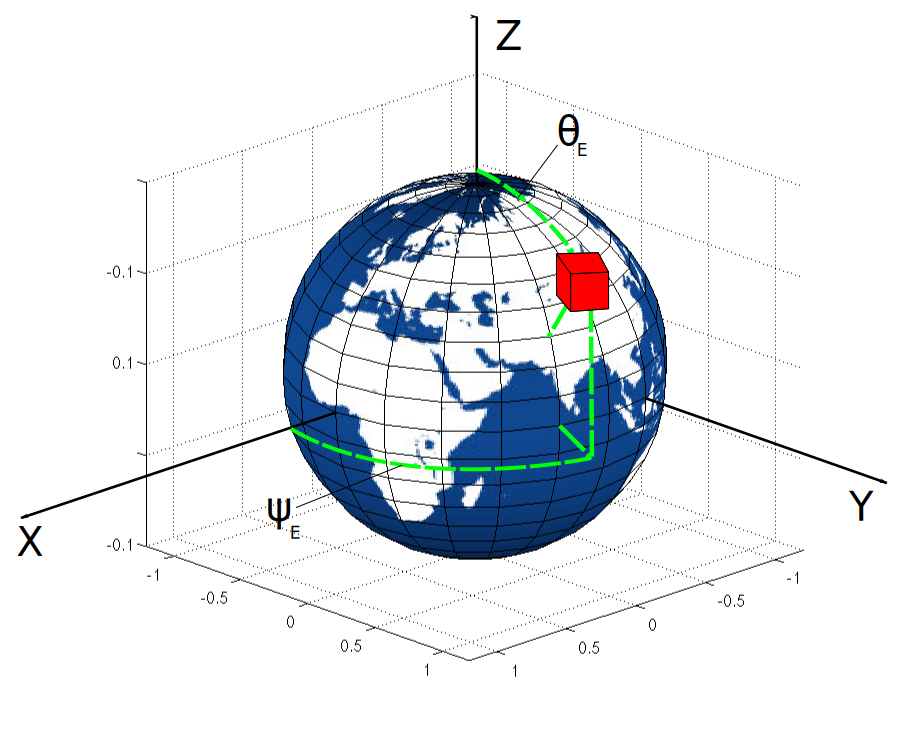
\includegraphics[height=100mm, width=120mm]{Figures/ECI.pdf}
  \end{center}
  \caption{Earth-Centered Inertial Frame and Spherical Coordinate Frame}\label{f:spherical}
\end{figure}
\noindent In order to connect these inertial coordinates ($x,y,z$) to
be used in the EMM2015 model, the latitude, longitude and height above
the surface of the Earth are required. To do this, the coordinates are
converted into spherical coordinates using the equations below.
\begin{equation}\label{e:spherical_coordinates}
  \begin{matrix}
    \rho = \sqrt{x^2+y^2+z^2} \\
    \phi_E = 0 \\
    \theta_E = cos^{-1}\left( \frac{z}{\rho}\right) \\
    \psi_E = tan^{-1}\left( \frac{y}{x}\right)
  \end{matrix}
\end{equation}
Note that $\rho,\phi_E,\theta_E,\psi_E$ are related to latitude and
longitude coordinates but not quite the same. In order to obtain the
latitude and longitude coordinates the following equations are
used. The height is simply the distance from the center of the ECI
frame minus the reference height from the approximation of Earth as an
ellipsoid ($R_{\Earth}=6,371,393~meters$). Note that the angles from Equation
\ref{e:spherical_coordinates} are converted to degrees. 
\begin{equation}
  \begin{matrix}
    \lambda_{LAT} = 90 - \theta_E\frac{180}{\pi}\\
    \lambda_{LON} = \psi_E\frac{180}{\pi} \\
    h = \rho - R_{\Earth}
  \end{matrix}
\end{equation}
The inputs to the EMM2015 model are the latitude, longitude and height. The inverse of the above two equations are given below. These would be used in the event a latitude and longitude coordinate is given and there is a need to obtain the x,y and z coordinates in the ECI frame. The first step is to convert latitude, longitude and altitude and convert that to standard spherical angles and distance from the center of the planet.
\begin{equation}
\begin{matrix}
\theta_E = (90 - \lambda_{LAT})\frac{\pi}{180}\\
\psi_E = \lambda_{LON}\frac{\pi}{180}\\
\rho = h + R_{\Earth}
\end{matrix}
\end{equation}
Once that is complete the extraction of x,y and z are computed by the equation below.
\begin{equation}
\begin{matrix}
x = \rho sin(\theta_E) cos(\psi_E)\\
y = \rho sin(\theta_E) sin(\psi_E)\\
z = \rho cos(\theta_E)
\end{matrix}
\end{equation}
The output from the EMM2015 model is in the East, North, Vertical (ENV) reference frame
where the x-axis is East pointing in the direction of the rotation on
the Earth, the y-axis is North pointing towards the North pole and
finally the z-axis is the Vertical component that is always pointing
radially away from the center of the Earth. In order to get the
coordinates into the ECI frame the coordinates must first me converted
to the North, East, Down reference frame (NED). In this case the
x-axis is pointing North, the y-axis pointing East and the z-axis is
always pointing towards the center of the Earth and called Down. The
equation to rotate from the ENV frame to NED frame is shown below.
\begin{equation}
  \begin{Bmatrix} \beta_x \\ \beta_y \\ \beta_z \end{Bmatrix}_{NED}
  = \begin{bmatrix} 0 & 1 & 0 \\ 1 & 0 & 0 \\ 0 & 0 & -1 \end{bmatrix} \begin{Bmatrix} \beta_x \\ \beta_y \\ \beta_z \end{Bmatrix}_{ENV}
\end{equation}
Once the magnetic field is in the NED reference frame it can then be
rotated to the inertial frame using the following equation where $\vec{\beta}_{NED}$ is the
magnetic field in the NED coordinate system and $\vec{\beta}_I$ is the
magnetic field in the inertial frame. 
\begin{equation}\label{e:sph_inertial}
  \vec{\beta}_I = {\bf T}_{IB}(0,\theta_E+\pi,\psi_E)\vec{\beta}_{NED}
\end{equation}
The matrix ${\bf T}_{IB}(\phi,\theta,\psi)$ represents the transformation
matrix from the spherical reference frame to the inertial reference
frame. Note that there is no rotation about the x-axis through
$\phi_E$ and the pitch rotation is augmented by $\pi$ because of the
switch between North, East, Down (NED) and the z-axis of the ECI
pointing through the North pole. The result of these equations, is the
ability to obtain the magnetic field  
across an entire orbit. Figure \ref{f:orbit} shows an example 56
degree inclination orbit, 600 km above the Earth's surface. The orbit
begins with the satellite above the equator and the prime meridian and
assumes the Earth does not rotate.
\begin{figure}[H]
  \begin{center}
  \includegraphics[height=70mm, width=80mm]{Figures/Earth_Orbit.png}
  \end{center}
  \caption{Example 56 Degree Inclination Orbit at 600 km above Earth's
  Surface}\label{f:orbit}
\end{figure}
Figure \ref{f:mag_orbit} shows the magnetic field during the orbit in the
inertial frame. PCI stands for Planet Centered Inertial which in this
case is the same as the ECI frame since the planet is Earth. 
\begin{figure}[H]
  \begin{center}
  \includegraphics[width=90mm]{Figures/Magnetic_Field_Orbit}
  \end{center}
  \caption{Magnetic Field of Earth in Inertial Frame for 56 Degree
    Orbit at 600 km Above Surface}\label{f:mag_orbit}
\end{figure}
For a satellite in LEO, the spacecraft will experience a magnetic
dipole moment. The magnetic dipole moment is caused by noting that the
structure of the satellite is metal with current that creates its own
magnetic field. The magnetic dipole moment torque is given by
computing the torque produced by the magnetic field of the Earth
interacting with the metallic structure of the satellite. First the
dipole constant $d_s=2.64E-03~N-m/T$ is the assumed value for torque
as a function of Tesla in LEO. This constant is derived by assuming
the torque from this disturbance at 500 km above the surface is the
same as the solar radiation torque. Using this constant, the torque is
given by the equation below where $\vec{\beta}_I$ is the magnetic
field strength of Earth in the inertial frame. The direction of the
torque is assumed to be in the same direction of the magnetic field
since the structure is not fully modeled. Although not accurate, the
goal is to approximate the magnitude as closely as possible.  
\begin{equation}
    \vec{M}_{MD}=\vec{\beta}_I d_s
\end{equation}

\subsection{Gravitational Models}

Three types of gravitational models can be used. The first is the
Newtonian gravitational model that assumes all planets are point
masses with no volume. The result of the gravitational field vector is
then
\begin{equation}
  \vec{F}_{\Earth} = -G\frac{m_{\Earth} m_s}{r^2}\hat{r}
\end{equation}
where $G$ is the gravitational constant, $\Earth$ denotes the planet
applying the gravitational field, $m_\Earth$ is the mass of the
planet, $m_s$ is the mass of the satellite and $\vec{r}$ is a distance
vector from the center of the planet to the satellite. The vector
$\hat{r}$ is just the unit vector of $\vec{r}$ while $r$ is the
magnitude of $\vec{r}$.
\begin{equation}
  \hat{r} = \vec{r}/r
\end{equation}
In component form, $\vec{r} = [x;y;z]^T$. Substituting that component
form into the two equations above results in the component form of the
gravity model which can be better suited for non-vectorized
programming syntax.
\begin{equation}
\begin{Bmatrix}F_{x\Earth}\\F_{y\Earth}\\F_{z\Earth}\end{Bmatrix} = -G\frac{m_{\Earth}
  m_s}{r^3}\begin{Bmatrix}x\\y\\z\end{Bmatrix}
\end{equation}
The second gravitational field model stems from the
Earth Gravity Model (EGM2008) \cite{EGM2008} which can also be found
in the GeographicLib module \cite{GeographicLib}. This model compute's
Earths gravitational field at any point in three dimensional
space. The model takes in coordinates in the ECI frame and returns the
gravitational acceleration in the ECI frame thus no rotation is
required. Just like the EMM2015 model this model uses spherical
harmonics and a reference ellipsoid. The reference ellipsoid is then
updated with gravity disturbances such as non-uniform geoid
heights. This model is an upgrade from EGM84 and EGM96 which only
used models of order 180 and 360 respectively. The EGM2008 model as a
comparison uses a model of order 2190. Figure \ref{f:grav_orbit} shows
the gravitational acceleration vector during a 56 degree orbit at 600 km above the
Earth's surface. The x-axis has been non-dimensionalized to 
represent the entire orbit. Thus when the x-axis is equal to 100 the
satellite has completed one orbit.
\begin{figure}[H]
  \begin{center}
  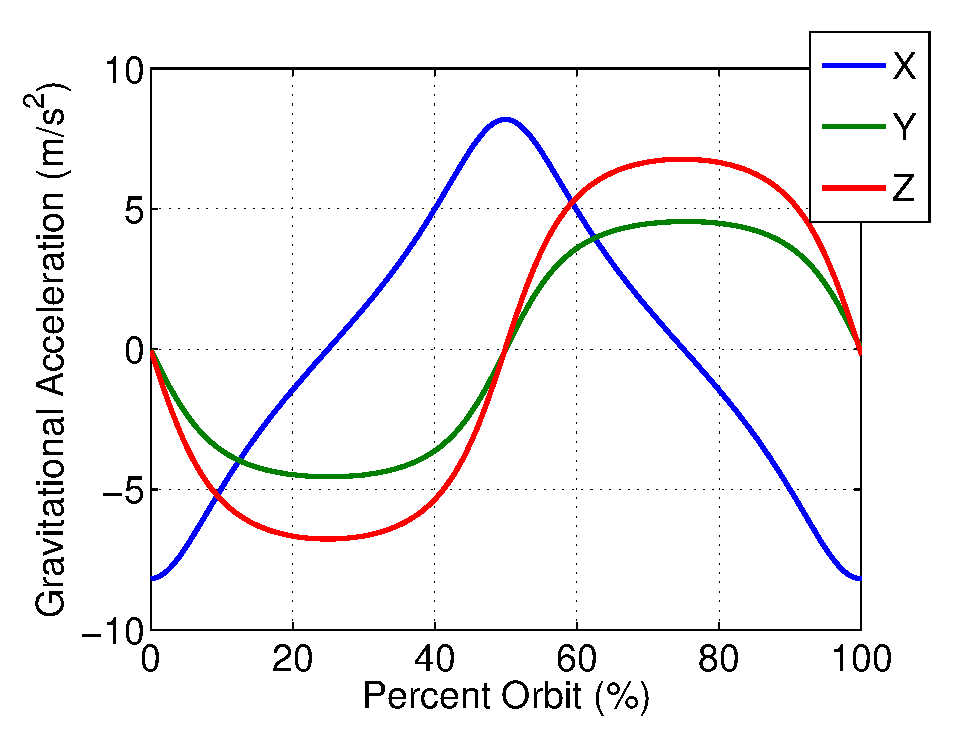
\includegraphics[height=80mm, width=100mm]{Figures/Gravity_Field_Orbit}
  \end{center}
  \caption{Gravitational Field of Earth in Inertial Frame for 56 Degree
    Orbit at 600 km Above Surface}\label{f:grav_orbit}
\end{figure}

For a satellite in LEO, the vehicle will experience a gravity gradient
torque. The gravity gradient torque is given by computing the
gravitational force at one end of the satellite and the other denoted
as $\vec{F}(\vec{r}_B)$ and $\vec{F}(\vec{r}_T)$ for bottom and top
respectively. The torques are then crossed with the distance from the
center of mass to the top of the satellite. It is assumed that the
satellite is symmetric and thus, the torque is just the difference
between the two forces crossed with the vector from the CG to one side
of the satellite. 
\begin{equation}
    \vec{M}_G = {\bf S}(\vec{F}(\vec{r}_B)-\vec{F}(\vec{r}_T))\vec{r}_{CG-B}
\end{equation}

The third gravitational field model assumes the vehicle is close to
the surface such as a quadcopter or aircraft. In this case the
gravitational field is held at a constant and equal to $9.81~m/s^2$.
\begin{equation}\label{e:wforce}
\begin{Bmatrix} X_W \\ Y_W \\ Z_W \end{Bmatrix} = mg \begin{Bmatrix}
-s_{\theta} \\ s_{\phi}c_{\theta} \\ c_{\phi}c_{\theta} \end{Bmatrix}
\end{equation}



\section{External Forces and Moments}

In addition to gravity acting on a vehicle, other forces also act
on the satellite. For a 1U CubeSat, the gravity gradient over 10 cm is about
$0.24~\mu m/s^2$ using the EGM2008 model. Multiplying this 
acceleration by a $1~kg$ mass and applying a $10~cm$ moment arm yields
a moment of about $2.4 \times 10^{-8}~N-m$. Aerodynamic torques could
be as large as $1.5 \times 10^{-10}~N-m$ assuming the aerodynamic
center is 5~cm away from the center of mass. Typical magnetorquers operate
in the vicinity of $3.0 \times 10^{-6}~N-m$, assuming a current of $0.04~A$, an area of
$0.02~m^2$, 84 turns and a magnetic field of $40,000~nT$. Using
these calculations, magnetorquers are two orders of magnitude
larger than gravity torques and four orders of magnitude larger than
aerodynamic torques. It is important to keep these values in mind when
neglecting certain parameters
\cite{Radiation,AndersonD,Density_Model}.

\subsection{Solar Radiation Pressure}

Solar radiation pressure is relatively constant at 1 AU and thus is
simply given as $p_s=4.5e-6~Pa$. The force is then found to be just
the pressure multiplied by the frontal area of the satellite. The
torque, similar to the aerodynamic torque, is the force crossed with a
distance vector from the center of mass to the center of pressure of
solar radiation. The vector $\hat{s}$ is a unit vector denoting the
direction of the sun.
\begin{equation}
  \vec{F}_{SR} = p_s S \hat{s}
  \end{equation}
\begin{equation}
    \vec{M}_{SR} = {\bf S} \left( \vec{F}_{SR} \right) \vec{r}_{CG-CPs}
\end{equation}

\subsection{Propulsion Model}

In order for a vehicle to lift off to enter space, engineers must be
able to apply a force that is greater than the force acting on the
vehicle due to gravity and aerodynamics.  The applied force is known
as thrust. Thrust can be generated by the propulsion system of the
vehicle. Electric and chemical are two well-known methods to produce
thrust which take advantage of Newton’s third law of motion.

Electric Propulsion Systems typically use electric heating or electric
or magnetic fields to accelerate propellants (usually gases).  These
systems can be very fuel-efficient, however it does not generate
enough thrust. These engines are great for deep space exploration
where transit times can be very long and rapid maneuvers are not
required\cite{qp8}.

Chemical propulsion systems are  more effective in our
environment. These systems involve the use of chemical reactions to
release energy and accelerate gases to produce thrust. Chemical
propulsion is a broad category and can be subdivided into liquid
propulsion, solid propulsion, and hybrid propulsion.

Liquid propulsion systems can be further subdivided into either a
monopropellant (a single propellant fluid) or a bi-propellant (two
fluids, which includes fuel and an oxidizer). The simplest form of
fuel and oxidizer would be liquid hydrogen and liquid
oxygen. Typically, the propellants may be kept on board and fed from
high-pressure tanks (pressure-fed) or use turbopumps to move the
propellant to the combustion  chamber (pump-fed) before the hot
exhaust exits the nozzle. Liquid Propulsion systems can produce a wide
range of thrust, can have high specific impulse (Isp), and can be
easily controlled; but often must be fueled shortly prior to launch.

On the contrary, solid rocket motors (or SRMs) are simple devices. The
propellants, the fuel and oxidizer, are mixed together and stored in a
cylinder. An electrical signal is sent to the igniter which creates
hot gases to ignite the main propellant grain. By converting the high
thermal energy of the gases into kinetic energy, therefore thrust is
developed. These motors usually have a relatively short burn time. For
example, The Thiokol motor using ammonium perchlorate/aluminum as
propellant, has a burn time of 75 s with a thrust of 3,300,000 lb.

Even though solid rocket motors are simple and can be ignited in a
moment's notice, their Isp  (specific impulse) is generally lower than
liquid systems. Also, they cannot be readily throttled. Once ignited,
the motor will burn to extinction\cite{qp9}. 

It is important to note, however, that if propulsion is needed for the
spacecraft it is necessary to work with the propulsion team to
determine the $\Delta V$,  mass flow rate, and attitude control. For
this analysis each satellite is equipped with $N_P$ thrusters that have a fixed
$I_{sp}$. The mass flow rate of each thruster is given by the equation
below where $p$ is the force of the thruster.
\begin{equation}
  \dot{m}_i = \sigma_i\frac{p}{9.81~I_{sp}}
\end{equation}
Each thruster is either on or off as given by the variable $\sigma$
which is either a 1 or a 0. When the thruster is on, the force
applied is equal to $p$ and when the thruster is off the thrust
applied is equal to zero. Thus in this fashion to total mass flow rate
per unit time of the entire satellite is just a sum of all the pulses.
\begin{equation}
  \dot{m} = \frac{p}{9.81~I_{sp}}\sum\limits_{i=1}^{N_P}\sigma_i
\end{equation}
It is assumed that the time response of the
thrusters is instantaneous during power up and power down. There is a
delay between pulses and the thrusters only stay on for a fixed time
thus the thrusters are pulsed in a square wave fashion with a certain
duty cycle. The force applied is simply equal to the force times a
unit vector that is aligned with the axis of the thruster. The total
force applied to each satellite is then given by the formula below.
\begin{equation}
  \vec{F}_P = p\sum\limits_{i=1}^{N_P}\sigma_i\hat{n}_{Pi}
\end{equation}
The total moment applied to the satellite is simply the force applied
crossed with a vector from the center of mass of the satellite to the
center of mass of the thruster.
\begin{equation}\label{e:propulsion}
  \vec{M}_P = p\sum\limits_{i=1}^{N_P}\sigma_i{\bf S}(\vec{r}_{Pi})\hat{n}_{Pi}
\end{equation}

\subsection{Magnetorquer Model}

The magnetorquer model assumes that three magnetorquers are aligned in
such a way that the magnetic moment produced by each magnetorquer is
aligned with the principal axes of the body frame of the
satellite. Each magnetorquer is controlled independently such that
$\vec{i}_M = [i_x,i_y,i_z]^T$ which is the applied current in each
magnetorquer. The magnetic moment is then given by the equation below 
\begin{equation}\label{e:magmoment}
  \vec{\mu}_M = nA\vec{i}_M
\end{equation}
where $n$ is the number of turns in the coil 
of each magnetorquer and $A$ is the area of the magnetorquer. For
simplicity it is assumed that all magnetorquers have the same area and
same number of turns. The torque produced by all magnetorquers is then
simply found by crossing the magnetic moment with the magnetic field
of the Earth in the Body reference frame.
\begin{equation}\label{e:magtorque}
  \vec{M}_M = {\bf S}(\vec{\mu}_M){\bf T_{BI}}(\vec{q})\vec{\beta}_I
\end{equation}
In order to obtain the magnetic field vector in the body frame, the
inertial magnetic field vector must be rotated into the body frame of
the satellite. In component form, equation (\ref{e:magtorque}) reduces to the following
equation using the identity that $\vec{a}\times\vec{b}=-\vec{b}\times\vec{a}$
\begin{equation}\label{e:magtorquecomponent}
  \begin{Bmatrix} L_M \\ M_M \\ N_M \end{Bmatrix} = nA\begin{bmatrix} 0 & \beta_z & -\beta_y \\ -\beta_z & 0 &
  \beta_x \\ \beta_y & -\beta_x & 0 \end{bmatrix}\begin{Bmatrix} i_{x}
    \\ i_{y} \\ i_{z} \end{Bmatrix}
\end{equation}
where $\beta_x,\beta_y,~\beta_z$ are the components of the magnetic
field in the body frame of the satellite. The moments $L,M,N$ are thus
the control torques that rotate the satellite as seen in equation
(\ref{e:pqrdot}).

\subsection{Aerodynamics}\label{s:aerodynamics}

Aerodynamics are typically written using a taylor series expansion
about a trim point\cite{phil}\cite{AndersonD}. That is, the aerodynamic forces are given by
\begin{equation}
\vec{F} = \vec{F}_0 + \frac{\partial \vec{F}}{\partial \vec{x}}(\vec{x}-\vec{x}_0)
\end{equation}
where $\vec{x} = [x,y,z,\phi,\theta,\psi,u,v,w,p,q,r]^T$. The partial
derivative is thus expanded such that
\begin{equation}
\frac{\partial \vec{F}}{\partial \vec{x}} = \begin{bmatrix} \frac{\partial
    \vec{F}}{\partial x} & \frac{\partial \vec{F}}{\partial y} & ... &
  \frac{\partial \vec{F}}{\partial r} \end{bmatrix}
\end{equation}
To find all of the partial derivative the forces are first written
using a combination of dynamic pressure and coefficients that are
functions of geometry and Reynolds number rather than speed, pressure
and size. A general lift force can be written using the equation below
\begin{equation}
L = \frac{1}2\rho {V_{\infty}}^2 S C_L
\end{equation}
where $\rho$ is the atmospheric density, $V_{\infty}$ is the
free-stream velocity, S is the planform area of the lifting surface and $C_L$ is
the lift coefficient. 
\begin{equation}\label{e:vtotal}
  V_{\infty} = \sqrt{{u_a}^2 + {v_a}^2 + {w_a}^2}
\end{equation}
The subscript 'a' above denotes the velocity of the vehicle plus the
atmospheric disturbance. 
\begin{equation}\label{e:atm}
\begin{Bmatrix} u_a \\ v_a \\ w_a \end{Bmatrix} =
\begin{Bmatrix} u \\ v \\ w \end{Bmatrix} +
{\textbf{T}^T}_{IB} \begin{Bmatrix}
 V_x \\ V_y \\ V_z \end{Bmatrix}
\end{equation}
Note that the dynamic pressure is different for vehicles other than aircraft. Note that the general form for drag is also very similar and can be written as
\begin{equation}
D = \frac{1}2\rho {V_{\infty}}^2 S C_D
\end{equation}
Specific sections are created below for other flying vehicles. A similar expression can be created for a
generic moment such that
\begin{equation}
M = \frac{1}2\rho {V_{\infty}}^2 S \bar{c} C_M
\end{equation}
where $\bar{c}$ is the mean chord of the lifting surface. The dynamic pressure $q_{\infty} =
\frac{1}2\rho {V_{\infty}}^2 S$ can be used to non-dimensionalize the forces, thus $L/q_{\infty} = C_L$. This means
that the equation involving partial derivatives can be written as
\begin{equation}
\frac{\partial \vec{C}_F}{\partial \vec{x}} = \begin{bmatrix} \frac{\partial
    \vec{C}_F}{\partial x} & \frac{\partial \vec{C}_F}{\partial y} & ... &
  \frac{\partial \vec{C}_F}{\partial r} \end{bmatrix}
\end{equation}
If the vector is then expanded to include the components of the vector
$\vec{F}$ the partial derivatives expand to
\begin{equation}
\frac{\partial \vec{C}_F}{\partial \vec{x}} = \begin{bmatrix}
  \frac{\partial C_X}{\partial x} & \frac{\partial C_X}{\partial y} &
  ... & \frac{\partial C_x}{\partial r} \\ \frac{\partial C_Y}{\partial x} & \frac{\partial C_Y}{\partial y} &
  ... & \frac{\partial C_Y}{\partial r} \\ \frac{\partial C_Z}{\partial x} & \frac{\partial C_Z}{\partial y} &
  ... & \frac{\partial C_Z}{\partial r} \end{bmatrix}
\end{equation}
shorthand can be adopted for the forces above such that
$\frac{\partial C_Y}{\partial x} = C_{Yx}$. Using this shorthand the
equation above can be written as.
\begin{equation}
\frac{\partial \vec{C}_F}{\partial \vec{x}} = \begin{bmatrix}
  C_{Xx} & C_{Xy} &
  ... & C_{Xr} \\ C_{Yx} & C_{Yy} &
  ... & C_{Yr} \\ C_{Zx} & C_{Zy} &
  ... & C_{Zr} \end{bmatrix}
\end{equation}
The coefficients listed above are standard coefficients that all
aircraft have. A similar matrix can be formulated for the moments on
an aircraft. When system identifying an aircraft all of these
coefficients may be determined. However, many of these terms are
zero. For example, all coefficients with respect to x y and z are
zero. That is, $C_{Xx} = C_{Yx} = ... C_{Nx} = C_{Xy} = ... C_{Nz} =
0$. Other coefficients can be set to zero as well but are not explicitly included in this text.

\subsubsection{Aircraft Aerodynamics}

For aircraft, some further simplifications are made. Some of the
coefficients defined above are combined to be written as functions of the
angle of attack($\alpha$) and sideslip($\beta$).
\begin{equation}\label{e:aoa}
\alpha = tan^{-1}\left(\frac{w_a} {u_a} \right)
\end{equation}
\begin{equation}\label{e:beta}
\beta = sin^{-1}\left(\frac{v_a}{V_{\infty}}\right)
\end{equation}
Transforming the equations into these formulations gives rise to
coefficients such as $C_{L\alpha}$ which is the change in lift as a
function of angle of attack and $C_{Y\beta}$ which is the change in
Y-Force as a function of sideslip. Using all of the coefficients
defined above taking into account the change to lift and drag, the body
aerodynamic force is calculated using the equation below.
\begin{equation}\label{e:aforce}
\begin{Bmatrix} X_A \\ Y_A \\ Z_A \end{Bmatrix} = \frac{1}2\rho
{V_{\infty}}^2 S \begin{Bmatrix}
C_Ls_{\alpha}-C_Dc_{\alpha}+C_{x_{\delta_t}} \delta_t
\\ C_{y{\beta}}{\beta}+C_{y{\delta}_r}{\delta}_r+C_{yp}\frac{pb}{2V_{\infty}}
+ C_{yr}\frac{rb}{2V_{\infty}} \\ -C_Lc_{\alpha}-C_Ds_{\alpha} \end{Bmatrix}
\end{equation}
Where the lift and drag coefficients are:
\begin{equation}\label{e:liftdrag}
\begin{Bmatrix} C_L \\ C_D \end{Bmatrix} = \begin{Bmatrix} C_{L0} +
C_{L\alpha}\alpha + C_{Lq}\frac{q\bar{c}}{2V_{\infty}} + C_{L\delta_e}\delta_e \\   C_{D0} +
C_{D\alpha}\alpha^2 \end{Bmatrix}
\end{equation}
The body aerodynamic moment is also computed using an aerodynamic expansion.
\begin{equation}\label{e:LMN}
\begin{Bmatrix} L_A \\ M_A \\ N_A \end{Bmatrix} = \frac{1}2\rho
{V_{\infty}}^2 S \bar{c} \begin{Bmatrix} C_{l\beta}\beta + C_{lp}\frac{pb}{2V_{\infty}} + C_{lr}\frac{rb}{2V_{\infty}} + C_{l\delta_a}{\delta_a} + C_{l\delta_r}{\delta_r}
\\  C_{m0} + C_{m\alpha}\alpha + C_{mq}\frac{q\bar{c}}{2V_{\infty}}+ C_{m\delta_e}\delta_e  \\ C_{np}\frac{pb}{2V_{\infty}} + C_{n\beta}\beta + C_{nr}\frac{rb}{2V_{\infty}} + C_{n\delta_a}\delta_a + C_{n\delta_r}\delta_r \end{Bmatrix}
\end{equation}
The aerodynamic coefficients in equations
(\ref{e:aforce}), (\ref{e:liftdrag}) and (\ref{e:LMN}) can be obtained from
flight data, aerodynamic modeling and windtunnel tests. Notice that
the only coefficients remaining are coefficients from angle of attack,
sideslip and angular velocities. Furthermore, the coefficients for
angular velocities are also non-dimensionalized by terms such as
$b/(2V_{\infty})$ where $b$ is the wingspan of the aircraft and
$\bar{c}$ is the mean chord of the aircraft. These terms are
introduced to fully non-dimensionalize the coefficients. Notice, as
well that four extra terms were also introduced. These will 
be discussed in more detail in the control section however the four
terms are the aileron control surface $\delta_a$, the elevator
control surface $\delta_e$, the rudder control surface $\delta_r$ and
the thrust control value $\delta_t$. 

\subsubsection{Projectile Aerodynamics}

To fully define the projectile aerodynamics some more assumptions are
made about the projectile.
\begin{enumerate}
\item The projectile is axially symmetric
\item The aerodynamic forces are not necessarily formulated at the center
  of mass
\item The projectile has the potential to be spinning rapidly thus
  interacting with the surrounding atmosphere
\end{enumerate}
For a projectile the dynamic pressure is written as
\begin{equation}\label{e:rocket_q}
Q = \frac{\pi}{8}\rho V_{\infty}^2d^2 
\end{equation}
The aerodynamic forces on the projectile are modeled using taylor series
ballistic expansions with known coefficients similar to the aircraft
model only slightly different assumptions are made given the dynamics
of the projectile. The subscripts in the equation below stand for
steady and unsteady aerodynamics.
\begin{equation}\label{e:aeroF}
\begin{Bmatrix} X_A \\ Y_A\\ Z_A \end{Bmatrix} = \begin{Bmatrix}
  X_{SA} \\ Y_{SA}\\ Z_{SA} \end{Bmatrix} + \begin{Bmatrix}
  X_{UA} \\ Y_{UA}\\ Z_{UA} \end{Bmatrix} = 
Q \begin{Bmatrix} -C_{X_0} - C_{X_2}\frac{v^2+w^2}{V^2}\\
-C_{Y_\beta}\frac{v}{V}\\
-C_{N_\alpha}\frac{w}{V}
\end{Bmatrix} + Q \begin{Bmatrix} 0
  \\ C_{Y_{p\alpha}}\frac{w}{V}\frac{pd}{2V} \\ C_{Z_{p\alpha}}\frac{v}{V}\frac{pd}{2V}\end{Bmatrix}
\end{equation}
In this equation, $Q$ is the dynamic pressure, $d$ is the aerodynamic
reference area, $C_{X_0}$ is the zero-yaw axial force
coefficient,$C_{X_2}$ is the yaw-squared axial force coefficient,
$C_{N_\alpha}$ is the normal force derivative coefficient,
$C_{Y_{p\alpha}}$ is the Magnus force coefficient, and
$V=\sqrt{u^2+v^2+w^2}$ is the total velocity of the projectile. 
The aerodynamic moments acting on the projectile are the pitching,
pitch damping, Magnus, and roll damping moments. Pitching and Magnus
moments are given by taking the cross product of the normal and Magnus
forces given in (\ref{e:aeroF})  with the position vector from the
center of mass to the center of pressure and location of Magnus force,
respectively. The total aerodynamic moments are given in
Eqn. (\ref{e:aeroM}). 
\begin{equation}\label{e:aeroM}
\begin{Bmatrix} L_A \\ M_A \\ N_A \end{Bmatrix}=
{\bf S}_B(\vec{r}_{CG,COP})\begin{Bmatrix}
  X_{SA} \\ Y_{SA}\\ Z_{SA} \end{Bmatrix} + {\bf S}_B(\vec{r}_{CG,MCOP})\begin{Bmatrix}
  X_{UA} \\ Y_{UA}\\ Z_{UA} \end{Bmatrix} + 
Qd \begin{Bmatrix}
C_{l_p} \frac{pd}{2V} \\
C_{m_q} \frac{qd}{2V}\\
C_{n_r} \frac{rd}{2V} \end{Bmatrix}
\end{equation}
Here, ${\bf S}_B(\vec{r}_{CG,COP})$ is the skew-symmetric operator
acting on the position vector from the center of mass to the center of
pressure expressed in the projectile body frame. Furthermore, ${\bf S}_B(\vec{r}_{CG,MCOP})$ is the skew-symmetric operator
acting on the position vector from the center of mass to the magnus
center of pressure expressed in the projectile body frame. Typically
the center of mass is defined from the rear of the projectile such
that 
\begin{equation}
{\bf C}_B(\vec{r}_{CG}) = \begin{Bmatrix} SL_{CG} \\ BL_{CG} \\ WL_{CG} \end{Bmatrix}
\end{equation}
Similarly, the center of pressure is defined from the rear of the
projectile such that
\begin{equation}
{\bf C}_B(\vec{r}_{COP}) = \begin{Bmatrix} SL_{COP} \\ BL_{COP} \\ WL_{COP} \end{Bmatrix}
\end{equation}
The vector $\vec{r}_{CG,COP}$ is then simply the different between
both vectors.
\begin{equation}
\vec{r}_{CG,COP} = \vec{r}_{COP}-\vec{r}_{CG}
\end{equation}
The damping coefficient defined in equation (\ref{e:aeroM})
include $C_{l_p}$ which is the roll damping coefficient while $C_{m_q}$ is the pitch damping
coefficient. These coefficients are added which essentially inhibit
angular motion of the projectile. In addition, to these coefficients,
sometimes magnus coefficients are given as pure moments rather 
than forces acting at a distance. This can be given in the equation
below. 
\begin{equation}
M_{UA} = Qd (-C_{M\alpha}\frac{v}{V} + C_{N_{p\alpha}}\frac{w}{V}\frac{pd}{2V})
\end{equation}
Where $C_{M\alpha}$ replaces the moment produced by $C_{N\alpha}$ and
$C_{N_{p\alpha}}$ replaces the moment produced by
$C_{Y_{p\alpha}}$. It is possible to derive an equation between the
two different representations as given by the equations below.

\begin{equation}
\begin{matrix}
C_{M\alpha} = \frac{(SL_{COP}-SL_{CG})C_{N\alpha}}{d} \\
C_{N_{p\alpha}} = \frac{(SL_{MAG}-SL_{CG})C_{Y_{p\alpha}}}{d}
\end{matrix}
\end{equation}

\subsubsection{Quadcopter Aerodynamics}

The aerodynamic model is based on a standard X-frame quadcopter as shown in the Figure below.
\begin{figure}[H]
\centerline{               
\includegraphics[width=11cm]
{Figures/Iris+QuadcopterDrawing.png}}
\caption{3DR Iris+ quadrotor model.}
\label{iris+}
\end{figure}
The forces exerted on the quadrotor are the total thrust and aerodynamic drag. 
\begin{equation}
\begin{Bmatrix}
X_{A}\\Y_{A}\\Z_{A}
\end{Bmatrix}= -T\begin{bmatrix}
0 \\ 0 \\ 1
\end{bmatrix} + \begin{Bmatrix}
X_{A_{D}} \\ Y_{A_{D}} \\ Z_{A_{D}}
\end{Bmatrix}
\label{XYZD}
\end{equation}
In Eq. (\ref{XYZD}), $T$ is the total thrust from the rotors and $\{X_{A_{D}}$,$Y_{A_{D}}$,$Z_{A_{D}}\}^{T}$ is the  total drag on the body. The total thrust exerted on the quadcopter is made possible due to the counter-rotating blades and allows for easy maneuverability by deviating the rotor angular velocities. The thrust can be simply defined as the sum of the exerted rotor forces $f_{i}$ such that
\begin{equation}
T = \sum\limits_{i=1}^4 f_{i} = f_{1}+f_{2}+f_{3}+f_{4}
\label{Tsimple}
\end{equation}
The thrust model of each rotor can then be equated to angular velocity of each rotor ($\Omega_i$). Where $k_t$ is a positive constant.
\begin{equation}
f_{i} = k_{t}{\Omega_{i}}^{2}
\label{fi}
\end{equation}
The total drag caused by the thrusting of the motors is a combination of the induced drag and rotor flapping \cite{quadfdnc}. The induced drag acting on the platform is caused by an imbalance in the thrust produced by advancing and retreating blades. This behavior can be modeled as a linear function of multirotor translational velocity in the quadcopter frame. Additionally, drag due to rotor flapping is caused by rotor flexibility, which is function of advance ratio and dependent on the rotor blades and hub design\cite{rotorflap}. Thus, the total drag vector on the quadcopter is expressed as
\begin{equation}
\begin{Bmatrix}
X_{A_{D}} \\ Y_{A_{D}} \\ Z_{A_{D}}
\end{Bmatrix} = -T\begin{Bmatrix}
\left(\frac{A_{1c}}{\eta} + d_{x}\right)u - \frac{A_{1s}}{\eta}v \\
\frac{A_{1s}}{\eta}u + \left(\frac{A_{1c}}{\eta}  + d_{y}\right)v \\ 0
\end{Bmatrix}
\label{DAxyz}
\end{equation}
where $d_{x}$, $d_{y}$ are the induced drag coefficients and $A_{1s}$,$A_{1c}$ are positive constants that describe the rotor flapping response as a function of advance ratio in Eq. (\ref{advanceratio})
\begin{equation}
\begin{split}
\mu = \frac{\sqrt{u^2 + v^2}}{\eta}\\
\eta = {\sum\limits_{i=1}^4 \Omega_{i}R}
\label{advanceratio}
\end{split}
\end{equation}
The quadcopter moment vector will consider additional aerodynamics created by the rotor torque.
\begin{equation}
\{L_A,M_A,N_A\}^{T}=  \overrightarrow{\Gamma} + \overrightarrow{\tau_{A}}
\label{LMNDT}
\end{equation}
For Eq. (\ref{LMNDT}),  $\overrightarrow{\Gamma}$ is the gyroscopic moment and $\overrightarrow{\tau_{A}}$ is the aerodynamic torque vector from the rotors. Note that $\overrightarrow{\tau_{A}}=\{\tau_{A_{\phi}},\tau_{A_{\theta}},\tau_{A_{\psi}}\}^{T}$ is the expanded form of the torque vector. The gyroscopic moments due to the rotors are defined as
\begin{equation}
\overrightarrow{\Gamma} = I_{r}\begin{bmatrix}
p \\ q \\ r
\end{bmatrix}\times\begin{bmatrix}
0 \\ 0\\ \Omega_{r}
\end{bmatrix} = \begin{bmatrix}
I_{r}\Omega_{r}q \\ -I_{r}\Omega_{r}p \\ 0
\end{bmatrix}
\label{Gamma}
\end{equation}
\begin{equation}
\Omega_{r} = \Omega_{1} - \Omega_{2} + \Omega_{3} - \Omega_{4} 
\label{Omegarel}
\end{equation}
where $I_{r}$ is the moment of inertia about the rotor axis and $\Omega_{r}$ is the relative rotor speed. In order to rotate the quadcopter to change its Euler angles, the angular velocitiis of each rotor can be altered. Due to the X-Frame design of the quadcopter, this text's convention is used to enumerate each rotor blade where rotor 1 is the forward-left rotor and the numbers continue in a clockwise fashion. The result is that the Euler angles are changed in a positive direction by noting the inequalities below.
\begin{equation}
\begin{split}
{\phi}^{+}: \Omega_{1}\Omega_{4} \textgreater \Omega_{2}\Omega_{3}\\
{\theta}^{+}: \Omega_{1}\Omega_{2} \textgreater \Omega_{3}\Omega_{4}\\
{\psi}^{+}: \Omega_{1}\Omega_{3} \textgreater \Omega_{2}\Omega_{4}
\label{ptpplus}
\end{split}
\end{equation}
Based on Eq. (\ref{ptpplus}), the torques are modeled accordingly as 
\begin{equation}
\begin{split}
\tau_{A_{\phi}} = l_{\phi}[(f_{1}+f_{4})-(f_{2}+f_{3})]\\
\tau_{A_{\theta}} = l_{\theta}[(f_{1}+f_{2})-(f_{3}+f_{4})]\\
\tau_{A_{\psi}} = \tau_{1}-\tau_{2}+\tau_{3}-\tau_{4}
\label{tauptp}
\end{split}
\end{equation}
In Eq. (\ref{tauptp}), $l_{\phi}$ and $l_{\psi}$ are the lengths from the rotor axis to the positive platform frame axes for roll and pitch, respectively. Positive yaw torque is achieved by reducing the angular velocity in rotors 2 and 4.  The torque ($\tau_i$) of each rotor is also modeled as a fucntion of the angular velocity.
\begin{equation}
\tau_{i} = b{\Omega_{i}}^{2}
\label{taui}
\end{equation}
The constant $b$ in the above equation denote the blade drag factor. The constants are modeled using blade element momentum theory\cite{swingload}. 
\begin{equation}
k_{t} = C_{T}\frac{4\rho {R}^{4}}{{\pi}^{2}}
\label{kt}
\end{equation}
\begin{equation}
b = C_{\tau}\frac{4\rho {R}^{5}}{{\pi}^{3}}
\label{b}
\end{equation}
In Eqs. \ref{kt} and \ref{b}, $\rho$ is the air density, $C_{T}$ is the thrust coefficient, and $C_{Q}$ is thetorque coefficient. 

\subsubsection{Spacecraft Aerodynamics}

The aerodynamic force is computed using aerodynamic coefficients and
dynamic pressure where $\vec{V}$ is the velocity of the satellite and
$V$ is the magnitude of the velocity vector. Furthermore, $S$ is the
surface area of the satellite and $C_D$ is the drag coefficient. The
torque on the satellite is then given by the cross product between the
aerodynamic force and a distance vector representing the distance
between the center of mass and the center of pressure
$\vec{r}_{CP-CG}$.
\begin{equation}
  \vec{F}_A = \frac{1}{2}\rho V\vec{V}S C_D
\end{equation}
\begin{equation}
    \vec{M}_A = -{\bf S}\left(\vec{F}_A\right)\vec{r}_{CP-CG}
\end{equation}

\section{Planetary Positions}\label{s:ephemeris}

Assuming that the Sun is the central inertial reference point, it is
possible to obtain the position of Earth and all the other planets at any point in time using 
well documented orbital elements of our solar system. This formulation
follows the derivation by JPL and can be found at \cite{JPL}.

\subsection{Julian Day}
In order to obtain the position of the planets, the Julian Day must be
obtained. The Julian Day of January 1st, 2019 is 2,458,485. The Julian
Day of January 1st, 2000 (which is the day of the last inertial frame
update) is 2,451,545. In order to obtain the Julian Day of the current
day, you simply need to count the number of calendar days from January
1st of 2000. Again I have listed the Julian day of January 1st, 2019
to help with this calculation. To compute the orbital elements of the
Earth you must then compute the number of centuries from January 1st,
2000 which is given by the equation below where J is the Julian day
and C is the number of centuries since 1/1/2000. 
\begin{equation}
  C = (J - 2,451,545)/36,525.0
\end{equation}

\subsection{Orbital Elements}
This number is then used in the equations below to obtain the current
semi-major axis, eccentricity, inclination, mean longitude, longitude
of perihelion and the longitude of the ascending node
respectively. The subscript $0$ denotes the orbital element in the
year 2000.
\begin{equation}
  \begin{matrix}
    a = (a_0 + \dot{a}C)AU \\
    e = e_0 + \dot{e}C \\
    i = i_0 + \dot{i}C \\
    L = L_0 + \dot{L}C \\
    \bar{w} = \bar{w}_0 + \dot{\bar{w}}C \\
    \Omega = \Omega_0 + \dot{\Omega}C
  \end{matrix}
\end{equation}
The parameters in the equation above for every planet can be found at
\cite{JPL}. Also, The term $AU$ is an astronomical unit which is equal
to 149,597,870,700 meters. For reference though the parameters for
Earth are shown below. Just in case you are reading this in the not so
distant future, these parameters are only valid until the year
2050 (I may be dead who knows!). Also, the parameters below are for the Earth-Moon barycenter 
which is the center of mass of the Earth and Moon.
\begin{table}
  \begin{center}
  \caption{Orbital Elements of Earth-Moon Barycenter}
\begin{tabular}{cccccc}
    a  &  e  & i & L & long.peri. ($\bar{w}$) & long.node. ($\Omega$)  \\
    \hline
    AU, AU/Cy &  rad, rad/Cy & deg, deg/Cy &  deg, deg/Cy & deg, deg/Cy &  deg, deg/Cy \\
    \hline 
    \hline 
    1.00000261 &  0.01671123  &  -0.00001531 &  100.46457166 &  102.93768193 &  0.0\\
    0.00000562 &  -0.00004392 &  -0.01294668 &   35999.37244981 &  0.32327364  &    0.0\\
    \hline
\end{tabular}
\end{center}
\end{table}
In the table, the first row is the value in the year 2000 and
the second row is the rate per century (Cy). Using these parameters,
compute the argument of the perihelion $w = \bar{w} - \Omega$ and the
mean anomaly $M = L - \bar{w}$. Note that for planets Jupiter, Saturn,
Uranus and Neptune, the mean anomaly has a different form. Basically
anything past the asteroid belt. With the mean anomaly compute you
must modulus this value such that M is between plus or minus 180
degrees. Once that's done you must solve for the eccentric anomaly (E)
using the Kepler equation below where $e^*$ is the eccentricity in
degrees $e^* = 180e/\pi$. 
\begin{equation}
  M = E-e^*sin(E)
\end{equation}
Solving this numerically is pretty simple and only requires a few
iterations of the loop below using the C++ programming language. This
loop can easily be adapted to any language on modern computers. C++ is
shown here in the event this is used for embedded processors in future
satellite systems. 
\begin{verbatim}
  E = M + e*180.0/PI*sin(M*PI/180.0);
  dM = 1;
  dE = 0;
  while (abs(dM) > 1e-6) {
    dM = M - (E - e*180.0/PI*sin(E*PI/180.0));
    dE = dM/(1.0-e*cos(E*PI/180.0));
    E += dE;
  }        
\end{verbatim}
\subsection{Sun Centered Inertial Coordinates}
At this point the spatial coordinates can be obtained in the planet's
orbital plane where the semi-latus rectum or sometimes simply called
the parameter is $p=a(1-e)$. 
\begin{equation}
  \begin{Bmatrix} x' \\ y' \\ z' \end{Bmatrix} = \begin{Bmatrix} a(cos(\pi E/180) - e)
    \\ a\sqrt{1-e^2}sin(\pi E/180) \\ 0 \end{Bmatrix}
\end{equation}
Notice that the value $z'$ is zero. This is because orbits are all two
dimensional. In order to obtain the coordinates of the planet in the
J2000 ecliptic plane, the equation below is used which is similar to
the standard Euler angle transformation matrix only the 3-1-3 rotation
sequence is used rather than 3-2-1. 
\begin{equation}
  \begin{Bmatrix} x \\ y \\ z \end{Bmatrix}_{J2000} = \begin{bmatrix} c_wc_{\Omega}-s_ws_{\Omega}c_i &
    -s_wc_{\Omega}-c_ws_{\Omega}c_i & 0
    \\ c_ws_{\Omega}+s_wc_{\Omega}c_i &
    -s_ws_{\Omega}+c_wc_{\Omega}c_i & 0 \\
    s_ws_i & c_ws_i & 0 \end{bmatrix} \begin{Bmatrix} x' \\ y' \\ z' \end{Bmatrix}
\end{equation}
Running through this formulation for all the planets in the Solar
System including Pluto it is possible to plot the position of all
planets. The figures below are for January 1st, 2019.
\begin{figure}[H]
  \begin{center}
  \begin{tabular}{cc}
  \includegraphics[height=70mm, width=80mm]{Figures/all_planets_isometric.pdf}&
  \includegraphics[height=70mm, width=80mm]{Figures/inner_planets_isometric.pdf}\\
  \includegraphics[height=70mm, width=80mm]{Figures/top_down_view_all_planets.pdf}&
  \includegraphics[height=70mm, width=80mm]{Figures/inner_planets_top_down.pdf}\\
  \end{tabular}
  \end{center}
  \caption{Position of Planets using Orbital Elements}
\end{figure}

\section{Linear Time Invariant Systems and Controls}

There is a branch of controls called Linear Time Invariant (LTI)
Systems that is often taught at the undergraduate level. Although
almost every system encountered in standard applications whether
aerospace or not are non-linear, it is still beneficial and more
simple to learn about control system dynamics when the system
parameters are constant and linear. 

\subsection{Linear Dynamics}

Standard nonlinear dynamics can be placed into standard
nonlinear affine form as shown below after much simplification of
terms
\begin{equation}
  \dot{\vec{x}} = \vec{f}(\vec{x}) + \vec{g}(\vec{x})\vec{u}
\end{equation}
where $\vec{u}$ is the control input which could be the forces and
moments from reaction wheels or thrusters. The equation above can be
linearized to give the equation below. 
\begin{equation}
  \Delta \dot{\vec{x}} = {\bf A}\Delta {\vec{x}} + {\bf B}\Delta \vec{u}
\end{equation}
where $\Delta \vec{x} = \vec{x} - \vec{x}_e$ and $\vec{x}_e$ is an
equilibrium point. In this formulation ${\bf A} = \partial \vec{f}/\partial \vec{x}$. and 
${\bf B} = \partial \vec{g}/\partial \vec{x}$ which are partial derivatives of the state matrices.

\subsection{Example Second Order System Formulation}

A second order system undergoing free motion will have dynamics that look like this
\begin{equation}
\ddot{q} + 2\zeta \omega_n \dot{q} + {\omega_n}^2 = \sigma f
\end{equation}
where $q$ is a generalized coordinate, $\sigma$ is a forcing term
proportional to the mass of the object and the forcing function $f$,
$\omega_n$ is the natural frequency of the system and $\zeta$ is the
damping ratio. Examples of these types of systems include mass, spring
dampers in linear translation as well as torsional systems and
penduluums. Anything that oscillates will exhibit this behavior. For a
standard mass spring damper system as shown in Figure \ref{f:msd}

\hl{INCLUDE MSD FIGURE}

\hl{INCLUDE MSD EOM FORMULATIONS}

\subsection{Solutions to Differential Equations}

\subsubsection{Characteristic and Particular Solutions}

\subsubsection{Laplace Solutions}

\subsection{Time Response of First and Second Order Systems}

\subsection{Proportional Derivative Integral Control}

\subsection{Lyapunov Control}

\subsection{Sliding Mode Control}

\subsection{Adaptive Control}

\subsection{Controllability}

Controllability is formally stated as a system where any initial
state $x(0)=x_0$ and final state $x_1,t_1>0$, there exists a piecewise
continuous input $u(t)$ such that $x(t_1)=x_1$. 
For a fixed wing aircraft the system has 12 states with 8 dynamic
modes and 4 zero or rigid body modes. For a fixed wing aircraft the system has 12 states with 8 dynamic
modes and 4 zero or rigid body modes. A conventional aircraft has 4
controls to control these 12 modes. The easiest way to test the 
controllability of a system  is to compute the
controllability matrix. However, the controllability matrix must be
computed using a linearized model such that
$\dot{\vec{x}}=A\vec{x}+B\vec{u}$. In order to do this the aircraft
must be in equilibrium. For this example the aircraft is
set with an initial velocity of $20~m/s$ at an altitude of
$200~m$. The altitude command is set to $200~m$ and the heading
command is set to zero. Given the zero heading angle command and the
symmetry of the configurations investigated the rudder and aileron
commands are set to zero. Thus, only the thrust and elevator controls
are activated for the trimming procedure. Each configuration is
simulated for 200 seconds or until the derivatives of all states
except $\dot{x}$ are within a required tolerance. Using this
equilibrium point a linear model can be computed by using forward
finite differencing assuming that the
aircraft model is put in the form $\dot{\vec{x}} = F(\vec{x},\vec{u})$.
\begin{equation}
\dot{\vec{\delta x}} = \frac{F(\vec{x_0}+\Delta \vec{x_0},\vec{u_0})-F(\vec{x_0},\vec{u_0})}{\Delta
  \vec{x}}\vec{\delta x} + \frac{F(\vec{x_0},\vec{u_0}+\Delta
  \vec{u})-F(\vec{x_0},\vec{u_0})}{\Delta \vec{u}}\vec{\delta u}
\end{equation}
This linear model is the classic linear model where
$\dot{\vec{\delta x}}=A\vec{\delta{x}}+B\vec{\delta{u}}$. Using this linear model, the
controllability matrix can be computed as
\begin{equation}
W_C = [B~AB~A^2B~A^3B~...~A^{N-1}B]
\end{equation}
where N is the number of states in the system. With the controllability
matrix formulated, the rank of the matrix is computed. If the
$rank(W_C)=N$ the system is said to be controllable.


\section{Numerical Integration Techniques}

\subsection{Euler's Method}

The equations of motion presented in this text as well as any
differential equation can be integrated using Euler's method
which is a crude first order method to approximate the time series
solution \cite{Chapra_MEANALYSIS}. Note that this method is prone to a 
significant amount of instability unless the timestep is very small. 
\begin{equation}
  \begin{matrix}
    \vec{x}_{k+1} = \vec{x}_k + \dot{\vec{x}}(t_k,\vec{x}_k) \Delta t \\
    \dot{\vec{x}}(t_k,\vec{x}_k) = \vec{f}(\vec{x}_k) + \vec{g}(\vec{x}_k)\vec{u}_k
  \end{matrix}
\end{equation}

\subsection{Runge-Kutta-4}

The RK4 algorithm is the standard in numerical integration and is
given in the equation below \cite{Chapra_MEANALYSIS}. The derivative
of the quaternions is the same in RK4 as it is in Euler's method. This
method is superior to RK4 in that it will converge faster as a
function of timestep.
\begin{equation}
  \begin{matrix}
    \vec{k}_1 = \dot{\vec{x}}(t_k,\vec{x}_k)\\
    \vec{k}_2 = \dot{\vec{x}}(t_k+\Delta t/2,\vec{x}_k+\vec{k}_1\Delta t/2)\\
    \vec{k}_3 = \dot{\vec{x}}(t_k+\Delta t/2,\vec{x}_k+\vec{k}_2\Delta t/2)\\
    \vec{k}_4 = \dot{\vec{x}}(t_k+\Delta t,\vec{x}_k+\vec{k}_3\Delta t)\\
    \vec{k} = \frac{1}{6}(\vec{k}_1 + 2\vec{k}_2 + 2\vec{k}_3 + \vec{k}_4)\\
    \vec{x}_{k+1} = \vec{x}_k + \vec{k} \Delta t \\
  \end{matrix}
\end{equation}

\subsection{Discrete Dynamics}

It is often useful for modern computers to write the equations of
motion in discrete form....

\section{Aerospace State Estimation}

\subsection{Sensor Measurement} \label{s:measurements}

During the standard estimation procedure, it is assumed that
measurements are made that relate to the state or the state is
directly measured. If the state is directly measured like star trackers no special formulation need to
made. However, other sensors such as Sun sensors, magnetometers and
horizon sensors measure a vector in 3-D space. In general a
measurement $\bar{y}_k$ can be expressed by the nonlinear equation
shown below where $\vec{x}$ is the state vector. 
\begin{equation}
  \bar{y}_k = \vec{h}(\vec{x}_k) + \vec{\nu}_k
\end{equation}
The vector $\vec{\nu}_k$ is noise associated with the sensor
\cite{Munoz,cassidis}. If the system is linearized about some
equilibrium point the measurement equation can be written as
\begin{equation}
  \bar{y}_k = {\bf h}_k\vec{x}_k + \vec{\nu}_k
\end{equation}
where ${\bf h}_k = \partial \vec{h}/\partial \vec{x}$. 
It's easy to see here that in the case of the star tracker the matrix
${\bf h}_k$ is just the identity matrix. The noise vector
$\vec{\nu}_k$ is assumed to be gaussian white noise while the
covariance $cov()$ is given by the equation below using the
expectation operator ${\bf E}()$.
\begin{equation}
  cov(\vec{\nu}_k) = {\bf E}(\vec{\nu}_k\vec{\nu}_k^T) = {\bf R}_k
\end{equation}
If a measurement is made by a
Sun sensor or similar where a vector in 3-D space can be compared to a
known inertial reference vector the measurement update can be given as 
\begin{equation}
  {\bar{r}^B}_k = {\bf T}_{BI}(\vec{q}_k){\vec{r}^I}_k + \vec{\nu}_k
\end{equation}
where ${\bar{r}^B}_k$ is a measurement in the body reference frame at
time $t_k$. The angular velocity measurement in particular can be denoted as
$\bar{\omega}_k$. Measurements are typically polluted with bias and
white noise. For example, the angular velocity measurement can be
given as
\begin{equation}
  \bar{\omega} = \vec{\omega} + \vec{b} + \vec{\eta}_g
\end{equation}
where $\vec{b}$ is a bias that has dynamics given by
$\dot{\vec{b}}=\vec{\eta}_b$. The vectors $\vec{\eta}_g$ and
$\vec{\eta}_b$ are standard Gaussian white noise vectors. Typically
white noise can be filtered out using lowpass filters, complimentary
filters or even Kalman Filters while bias can just be
substracted. Thus, the estimate for the angular velocity can be
written as
\begin{equation}
  \tilde{\omega} = \bar{\omega}-\tilde{b}
\end{equation}
where $\tilde{b}$ is the estimate of the bias.

\subsection{Linear Least Squares}

In order to understand the nature of a Kalman filter, the linear least
squares solution is shown below. Assume for the moment that $M$
independent measurements are made such that $\bar{Y} = [\bar{y}_1,...,\bar{y}_M]^T$.
\begin{equation}
  \bar{Y} = {\bf H}\vec{x} + \vec{V}
\end{equation}
In this case ${\bf H} = [{\bf h}_1,...,{\bf h}_M]^T$ and $\vec{V} = [\nu_1,...,\nu_M]^T$. 
The vector $\vec{V}$ is a vector of error values between your
measurements and the actual truth signals $Y = {\bf H}\vec{x}$. Absent
of all measurement and model noise there 
would be a unique solution to this problem to solve for the vector
$\vec{x}$. The matrices $\bar{Y}$ and {\bf H} are
known and are the measurements and the output equation relating the
measurements to the state values in $\vec{x}$ respectively. Because of
measurement and model noise, a unique solution is not possible. That
is, the problem is overconstrained since typically the number of measurements is larger
than the number of unknowns. Take the linear example as shown in the
figure below.
\begin{figure}[H]
  \begin{center}
  \includegraphics[height=80mm, width=100mm]{Figures/Linear_Regression.png}
  \end{center}
  \caption{Linear Regression Example}\label{f:linear_regression}
\end{figure}
In this case the ordinate axis is the output $Y$ and the abscissa is
the independent variable that characterizes the matrix ${\bf H}$. The
black dots then are the measurements $\bar{Y}$ while the trend line is
the estimate $\tilde{Y} = {\bf H}\tilde{x}$. In this case the residuals
$\hat{Y} = \tilde{Y}-\bar{Y}$ is the distance between the trend line
in red and the black dots (the measurements). For this linear example,
the unknowns would be the slope and intercept. It is clear here that
there exists no linear solution $\vec{x}$ that goes through all black
data points. Thus, the equation below can be constructed.
\begin{equation}
  \bar{Y} = {\bf H}\tilde{x} + \hat{Y}
\end{equation}
This implies that the trendline $\tilde{Y}$ would go through all data
points if $\hat{Y}$ were zero. Thus the solution to this problem was
originally found by Gauss \cite{stigler1981} and involved minimizing
the residuals between $\bar{Y}$ and $\tilde{Y}$ (the estimated Y
values). To do this, a cost function is generated such that
\begin{equation}
  J = \frac{1}{2}\hat{Y}^T \hat{Y}
\end{equation}
Substituting in the equation $\hat{Y} = \bar{Y} - {\bf H}\tilde{x}$
and minimizing the cost function $\partial J/\partial \tilde{x} = 0$
results in the solution below.
\begin{equation}
  \tilde{x} = ({\bf H}^T{\bf H})^{-1}{\bf H}^T\bar{Y}
\end{equation}
Note that the equation above only works if the number of measurements $M$
is greater than or equal to the number of unknowns $N$. If not, the
solution will always be rank deficient and no solution will be
found. This is called an under constrained problem. In this there are
an infinite number of solutions that satisfy $\bar{Y} = {\bf
  H}\vec{x}$ even in the presence of modeling errors. In order
to get around this issue Lagrange's method of 
optimization is used \cite{lagrange}. For problems like this the
residuals between the estimate $\tilde{Y}$ and the measured signals
$\bar{Y}$ can be easily made to be zero. Thus minimizing the residuals
is trivial since the solution will still be an infinite number of
solutions. Therefore a constraint can be placed where
$\bar{Y}=\tilde{Y}={\bf H}\tilde{x}$. In order to find a unique
solution then the requirement is placed to minimize the estimate
$\tilde{x}$. In this case, the cost function
to be minimized is given by Lagrange's extension to optimization as
shown below
\begin{equation}
L = \frac{1}{2}\tilde{x}^T\tilde{x} + \lambda^T(\bar{Y}-{\bf H}\tilde{x})
\end{equation}
The cost function above utilizes the method of Lagrange multipliers in
order to satisfy the constraint that the solution must pass through
all measurements again only if the number of measurements $M$ is less than
the number of unknowns $N$. In the equation above the vector
$\tilde{x}$ must be solved and so must the Lagrange multipliers
$\lambda$. The solution to the problem above requires
$\partial L / \partial \tilde{x} = 0$ and $\partial L / \partial \lambda = 0$. Carrying out the partial derivatives and solving for the estimate
yields the following equations. 
\begin{equation}
  \tilde{x} = {\bf H}^T({\bf H}{\bf H}^T)^{-1}\bar{Y}
\end{equation}
Note, it is standard practice in state estimation to have at least as
many measurements as unknowns. In this case $M=N$ and Gauss' solution
is sufficient. 

\subsection{Weighted Least Squares}

The weighted least squares solution is found by setting the cost
function equal to $J = \frac{1}{2}\hat{Y}^T{\bf W}\hat{Y}$
where {\bf W} is a positive definite and symmetric weighting matrix. The solution then is
shown below.
\begin{equation}\label{e:weights}
  \tilde{x} = ({\bf H}^T{\bf W}{\bf H})^{-1}{\bf H}^T{\bf W}\bar{Y}
\end{equation}
In the standard Kalman Filter approach, the weighting matrix is given
by the inverse covariance of the error ${\bf r} = {\bf
  E}[\vec{v}\vec{v}^T]$. Placing this into a matrix yield ${\bf W} =
{\bf R}^{-1}$ where ${\bf R} = diag([{\bf r}_1,...{\bf r}_M])$.  
The weighted least squares solution then reduces to
\begin{equation}
  \tilde{x} = ({\bf H}^T{\bf R}^{-1}{\bf H})^{-1}{\bf H}^T{\bf R}^{-1}\bar{Y}
\end{equation}

\subsection{A Priori Knowledge of the State Vector}

If a priori knowledge is obtained via other means or in the case of
the standard Kalman Filter from integration of the state, it is
possible to obtain an updated estimate of the state based on the
previous state estimate and the new sensor measurements. First, the a
priori estimate $\tilde{x}^{-}$ is written as 
\begin{equation}
  \tilde{x}^{-} = \vec{x} +  \vec{w}
\end{equation}
where $\vec{w}$ is model noise associated with the error in the
state estimate. The covariance of this noise is also denoted as a
matrix and defined below.
\begin{equation}
  cov(\vec{w}) = {\bf E}(\vec{w}\vec{w}^T) = {\bf q}
\end{equation}
In this case it is desired for the updated measurement to be some
linear combination of the a priori equation and the measurements such
that
\begin{equation}
  \tilde{x} = {\bf \Lambda}\bar{Y} + {\bf \Gamma}\tilde{x}^{-}
\end{equation}
The matrices ${\bf \Lambda}$ and ${\bf \Gamma}$ have an added constraint
which can be shown by assuming the a priori measurement is perfect
$\tilde{x}^- = \vec{x}$ and the measurements $\bar{Y} = Y = {\bf
  H}\vec{x}$. In this case, we must have the updated estimate equal
the truth signal. $\tilde{x} = \vec{x}$. Rearranging the equation above yields
\begin{equation}
  \vec{x} = {\bf \Lambda}{\bf H}\vec{x} + {\bf \Gamma}\vec{x}
\end{equation}
which means that $({\bf \Lambda}{\bf H} + {\bf \Gamma}) = {\bf I}$
Again using the method of lagrange multipliers the cost function to be
minimized is given as
\begin{equation}
  L = {\bf E}[\frac{1}{2}\hat{x}^T\hat{x} + \lambda^T({\bf I} - {\bf
    \Lambda}{\bf H} - {\bf \Gamma})]
\end{equation}
where $\hat{x} = \tilde{x} - \vec{x}$ and again {\bf E} is the
expectation operator. Remembering that {\bf q} is
the covariance of the model noise and {\bf r} is the covariance of the
measurement noise, the solution to the minimization problem is given
by the equation below. 
\begin{equation}
  \tilde{x} = ({\bf H}^T{\bf R}^{-1}{\bf H}+{\bf q}^{-1})^{-1}({\bf
    H}^T{\bf R}^{-1}\bar{Y}+{\bf q}^{-1}\tilde{x}^{-})
\end{equation}
Note that this solution assumes that ${\bf E}(\vec{w}\vec{v}^T) = 0$. Measurement and model noise are uncorrelated.

\subsection{Complimentary Filter}

Looking at the equation for the A priori knowledge it is possible to
formulate the complimentary filter. First, the measurements are
assumed to be identical to the state vector such that ${\bf h}_k = {\bf
  I}$. From here a few extremes are shown below. First, assume that the measurement error is very low such
that the $cov(\vec{\nu})<<1$ while the model noise $\vec{w}$ is very
large approaching infinity. In this case, ${\bf q}^{-1} =0$. Substituting this into the weighted apriori equation yields
\begin{equation}
  \tilde{x} = average(\bar{Y})
\end{equation}
which essentially states that the estimate completely believes the
sensor measurement. If instead we assume that the model noise is
perfect such that $cov(\vec{w})<<1$ and the sensor noise is
approaching infinity, then ${\bf R}^{-1}=0$. This yields the following equation.
\begin{equation}
  \tilde{x} = \tilde{x}^{-}
\end{equation}
Thus it can be seen that there is a sliding bar between believing the
apriori estimate or the sensor measurement. As such it is possible to
develop a much simpler filter. First a constraint is placed on {\bf q}
and {\bf R} such that
\begin{equation}
  ({\bf H}^T{\bf R}^{-1}{\bf H}+{\bf q}^{-1}) = {\bf I}
\end{equation}
This causes the update law to reduce to the following
\begin{equation}
  \tilde{x} = {\bf H}^T{\bf R}^{-1}\bar{Y}+{\bf q}^{-1}\tilde{x}^{-}
\end{equation}
If only one measurement is investigated the equation collapses to the
following.
\begin{equation}
  \tilde{x} = {\bf r}^{-1}\bar{y}+{\bf q}^{-1}\tilde{x}^{-}
\end{equation}
The constraint also collapses to
\begin{equation}
  {\bf r}^{-1}+{\bf q}^{-1} = {\bf 1}
\end{equation}
If ${\bf q}^{-1} = {\bf s}$ and ${\bf r}^{-1}={\bf 1}-{\bf s}$ the
update law simplifies to
\begin{equation}
  \tilde{x} = ({\bf 1}-{\bf s})\bar{y}+{\bf s}\tilde{x}^{-}
\end{equation}
Here it is clear that if ${\bf s} = {\bf 1}$ the new estimate will be
equal to the old estimate meaning that the sensor noise is approaching
infinite. If ${\bf s} = 0$ it means that the new estimate is equal to
the sensor measurement meaning the model noise is approaching
infinity. This is a simple crude first order filter that can be used
when only a simple understanding of covariance is known.

\subsection{Sequential Linear Estimator}

In the above two scenarios, it is assumed that all measurements from 1
to $M$ are known at the same time instant $t$ and thus the least squares estimate can be done ``all
at once". For discrete time sensors on board a spacecraft this is
not possible. For example, if we take the weighted least squares
solution assuming we have a {\it 0th} batch of measurements, the
estimate of $\tilde{x}$ would be
\begin{equation}
  \tilde{x}_0 = ({\bf h}_0^T{\bf w}_0{\bf h}_0)^{-1}{\bf h}_0^T{\bf
    w}_0\bar{y}_0
\end{equation}
If we then waited $\Delta t$ seconds for a new set of measurements we
would have to obtain a new estimate of $\tilde{x}$ which could be done
using the equation below
\begin{equation}
  \tilde{x}_1 = ({\bf h}_1^T{\bf w}_1{\bf h}_1)^{-1}{\bf h}_1^T{\bf
    w}_1\bar{y}_1
\end{equation}
This solution however would only take into account the new
measurements. Thus, if larger matrices were constructed like
${\bf H} = [{\bf h}_0,{\bf h}_1]$ the solution for $\tilde{x}$ becomes
the same as it was in Equation \ref{e:weights}. This process would be
tedious if these matrices were computed over and over again. This is
because the matrices would continue to grow larger and larger over
time and eventually overflow the memory management system on the
computer. Thus, a method for updating the state vector every time
a new measurement is obtained must be derived. To do this the two
equations are substituted into equation \ref{e:weights}. Then a
covariance matrix is used such that ${\bf p} = ({\bf h}^T{\bf w}{\bf h})^{-1}$ 
which never grows in size. Using that simplification and making use of
a estimation gain matrix ${\bf k}$, the estimation algorithm is as follows:
\begin{enumerate}[itemsep=-5pt]
    \item The first measurement is obtained $\bar{y}_0$
    \item Compute the matrix ${\bf p_0} = ({\bf h}_0^T{\bf w_0}{\bf h}_0)^{-1}$
    \item Obtain the estimate for $\tilde{x}_0 = {\bf p_0}{\bf
      h}_0^T{\bf w_0}\bar{y}_0$ (Notice that if you use the equation
      above this is the same solution as the weighted least squares estimate)
    \item Every time a new measurement, $\bar{y}_k$, is obtained use the recursive least squares update law shown in the equation below.  
\end{enumerate}
\begin{equation}
  \begin{matrix}
    {\bf k}_{k+1} = {\bf p}_{k}{\bf h}_{k+1}^T[{\bf h}_{k+1}{\bf p}_k{\bf h}_{k+1}^T+{\bf w}_k^{-1}]^{-1}\\
    {\bf p}_{k+1} = [{\bf 1} - {\bf k}_{k+1}{\bf h}_{k+1}]{\bf p}_k\\
    \tilde{x}_{k+1} = \tilde{x}_k + {\bf k}_{k+1}(\bar{y}_{k+1} - {\bf h}_{k+1}\tilde{x}_k) \\
  \end{matrix}
\end{equation}
In the special case where the weighting matrix
${\bf w}_k$ is equal to a constant ${\bf w}$ and the state vector is
directly measured such that ${\bf h}_k$ is also identity, the 
sequential linear estimator gives the following simplified steps.
\begin{enumerate}[itemsep=-5pt]
    \item The first measurement is obtained $\bar{y}_0$
    \item Compute ${\bf p}_0 = {\bf w}^{-1}$
    \item Obtain the estimate for $\tilde{x}_0 = \bar{y}_0$ (this is a fault of ${\bf h}_k$ being identity) 
    \item Every time a new measurement, $\bar{y}_k$, is obtained use the recursive least squares update law shown in the equation below.  
\end{enumerate}
\begin{equation}
  \begin{matrix}
    {\bf k}_{k+1} = {\bf p}_k[{\bf p}_k + {\bf w}^{-1}]^{-1}\\ 
    {\bf p}_{k+1} = [{\bf 1} - {\bf k}_{k+1}]{\bf p}_k\\
    \tilde{x}_{k+1} = \tilde{x}_k + {\bf k}_{k+1}(\bar{y}_{k+1} - \tilde{x}_k) \\
  \end{matrix}
\end{equation}

\subsection{The Continuous Time Complimentary Filter}

In the above section a discrete sequential least squares update law
was formulated. In that derivation it is assumed that the state
estimate is held constant in between state measurements. It is
possible however to integrate a model of the state dynamics and use
that estimate in between state measurements. The is the start of a
Kalman Filter. To formulate the Continuous Time Complimentary Filter
the dynamics of the system are written such that
\begin{equation}
  \begin{matrix}
    \dot{\vec{x}} = {\bf f}\vec{x} + {\bf g}u +{\bf m}\vec{w} \\
    \vec{y} = {\bf h}\vec{x}
  \end{matrix}
\end{equation}
where the initial conditions are $\vec{x}_0$ and $\vec{w}$ is a
modeling noise term where ${\bf E}[\vec{w}\vec{w}^T]={\bf q}$ just as
was defined in the a priori estimation section. The model dynamics are
set up such that 
\begin{equation}
  \begin{matrix}
    \dot{\tilde{x}} = \tilde{{\bf f}}\tilde{x} + \tilde{{\bf g}}u + \vec{\gamma}\\
    \tilde{y} = {\bf h}\tilde{x} \\
    \bar{y} = {\bf h}\vec{x} + \vec{v}
  \end{matrix}
\end{equation}
where again $\bar{y}$ is the state measurement and $\vec{v}$ is noise
associated with the sensor where {\bf E}$[\vec{v}\vec{v}^T]=${\bf
  r}. The term $\vec{\gamma}$ is added as a psuedo control which can
be whatever we want. The idea is for $u$ to be the control input to
drive $\vec{x} \rightarrow \vec{x}_c$ while the psuedo control is for
the observer dynamics to drive $\tilde{y} \rightarrow \bar{y}$. The
model dynamics are going to deviate in between sensor measurements so
if the observer dynamics are designed properly the estimate can
converge to the measurement. Of course, this means your estimate is
only as good as your measurement noise but it is a start. To design
the psuedo control law, measurement feedback is used in the same form
as standard unity feedback control laws such that $\vec{\gamma} =
{bf k}\hat{y}$ where $\hat{y}$ is the difference between the estimate and
the measurement. The closed loop dynamics can then be written as
\begin{equation}
  \dot{\tilde{x}} = (\tilde{{\bf f}}-{\bf k}{\bf h})\tilde{x} + \tilde{{\bf g}}u
  + {\bf k}\bar{y}
\end{equation}
Looking at this equation it's hard to see the effect of the
observer. Thus the error dynamics must be investigated where
$\hat{x}=\tilde{x}-\vec{x}$. For the simple case it is assumed that
${\bf f}=\tilde{{\bf f}}$ and ${\bf g}=\tilde{{\bf g}}$. The closed
loop error dynamics can then be written as
\begin{equation}
  \dot{\hat{x}} = ({\bf f} - {\bf k}{\bf h})\hat{x} + {\bf k}\vec{v}
\end{equation}
in this case the solution to this equation is
\begin{equation}
  \hat{x}(t) = \hat{x}_0e^{({\bf f} - {\bf k}{\bf h})t} + \vec{\eta}
\end{equation}
where the term $\vec{\eta}$ is a function of the noise term ${\bf
  k}\vec{v}$. In this case, if {\bf k} is chosen to be large, the
error dynamics will be very fast but the noise term will be very
large. If {\bf k} is chosen to be very small the error dynamics will
be slow but the error term will not be a prevalent. The issue with
this filter of course comes with how to tune the gain matrix {\bf k}
which is what the Kalman filter seeks to address.
   
\subsection{The Continuous Discrete Kalman Filter}

In the case of the continuous discrete Kalman Filter, the model
dynamics are integrated just as in the complimentary filter. The only
difference is instead of using a continuous observer the state
estimate is updated every time a new measurement is obtained much like
the sequential least squares technique. First, let's write the model
dynamics as before without the observer and the measurement equations
are written such that the measurement is taken at timestep $t_k$ and
thereafter every $\Delta t$. 
\begin{equation}\label{e:model_dynamics}
  \begin{matrix}
    \dot{\tilde{x}} = \tilde{{\bf f}}\tilde{x} + \tilde{{\bf g}}u \\
    \tilde{y} = {\bf h}\tilde{x} \\
    \bar{y}_k = {\bf h_k}\vec{x}(t_k) + \vec{v}_k
  \end{matrix}
\end{equation}
The update equation is written using the continuous observer dynamics
used for the complimentary filter only in this case the update is
discrete.
\begin{equation}\label{e:state_update}
  \tilde{x}_k^+ = \tilde{x}_k^- + {\bf k}_k(\bar{y}_k-{\bf
    h_k}\tilde{x}_k^-)
\end{equation}
In this case $\tilde{x}_k^+$ is the estimated state after the update
while $\tilde{x}_k^-$ is the estimate before the update. The equation
for the covariance update and the Kalman Gain matrix are identical in
that the derivation is formulated just as it was before. The equations
are shown below again only $+$ and $-$ is used to denote the matrices
before and after update.
\begin{equation}\label{e:kalman_gain}
  \begin{matrix}
  {\bf k}_{k} = {\bf p}_{k}{\bf h}_{k}^T[{\bf h}_{k}{\bf p}_k^-{\bf h}_{k}^T+{\bf r}]^{-1}\\
  {\bf p}_{k}^+ = [{\bf 1} - {\bf k}_{k}{\bf h}_{k}]{\bf p}_k^-
  \end{matrix}
\end{equation}
In the sequential linear estimator however, the covariance matrix was
set using a weighted least squares approach. In this case the
covariance matrix is set such that ${\bf p} = {\bf
  E}[\hat{x}\hat{x}^T]$. Taking a derivative of this equation and
substituting in the closed loop error dynamics yields the covariance
propagation equation shown below.
\begin{equation}\label{e:covariance_dynamics}
  \dot{{\bf p}} = \tilde{{\bf f}}{\bf p} + {\bf p}\tilde{{\bf f}}^T +
      {\bf m}{\bf q}{\bf m}^T
\end{equation}
The final Continuous Discrete Kalman Filter then goes like this.
\begin{enumerate}
  \item Integrate the model dynamics in Equation
    \ref{e:model_dynamics} and the covariance dynamics in equation
    \ref{e:covariance_dynamics}
  \item When a measurement is received, the Kalman Gain matrix is
    computed using equation \ref{e:kalman_gain}. 
  \item Equation \ref{e:kalman_gain} is also used to update the
    covariance matrix
  \item Finally, equation \ref{e:state_update} is used to update the
    state vector estimate and then the process repeats.
\end{enumerate}
An example figure is shown below for a first order system. In this
figure the blue stars represent discrete sensor measurements with some
noise. Everytime the sensor is updated the model performs and update
and instantaneously changes to a new value. The model then integrates
(incorrectly due to model mismatch) until a new sensor measurement is
obtained. In this case the model is so inaccurate it makes more sense
to update the sensor more frequently or perform some sort of adaptive
control algorithm to estimate the plant dynamics.
\begin{figure}[H]
  \begin{center}
    \includegraphics[height=80mm, width=140mm]{Figures/Kalman_Filter_Example.png}
  \end{center}
  \caption{First Order Kalman Filter Example}\label{f:kalman}
\end{figure}
    
\subsection{Kalman Filter for Spacecraft Dynamics}

Attitude estimation involves a combination of attitude determination
and state estimation. Assuming at time $t=t_0$ the attitude estimation
algorithm is performed and an estimate of the quaternion is obtained
as $\tilde{q}_0$. If discrete regular angular velocity
($\bar{\omega}_{k}$) measurements are made every $\Delta t$ seconds,
the quaternion can be estimated by simply integrating the attitude
equations of motion. Even if perfect sensor measurements are made, it
is possible to integrate these equations of motion over time and the
quaternion $\vec{q}$ will be much different than the estimated
quaternion $\tilde{q}$. Thus, the attitude estimation algorithm can
run again to obtain a new absolute quaternion measurement. The
equations of motion are integrated and when a new sensor measurement
is obtained the estimated state is updated based on the estimated
covariance combined with and estimate of model errors and sensor
errors. Finally, it is possible to 
create an Extended State Kalman Filter (EKF) which can estimate
sensor inaccuracies simply by finding the least squares solution
between the sensor measurements and state estimates. The sections that
follow details the Kalman Filter for Spacecraft Dynamics as well as
the extended state version which estimate bias values in the rate gyro.
  
First, the 4-dimensionality of the quaternion renders the
above Kalman filter formulation to be impossible mostly because the
quaternion derivative is a 4 by 1 matrix while the angular velocity
vector is a 3 by 1. Furthermore, the quaternion derivative is not
linear and cannot be expressed as the linear matrices in the previous
section. As such the Kalman Filter must be updated somewhat. The
derivative of the state $\dot{\vec{q}}$ is cumbersome and follows the
reference in \cite{Liu_Estimation}. First the angular 
velocity measurement is substituted into the derivative of
quaternions where the ${\bf \Omega}()$ and ${\bf \chi}()$ identity is used to
separate out the white noise parameter.
\begin{equation}
  \dot{\vec{q}} = \frac{1}{2}{\bf \Omega}(\vec{\omega})\vec{q} =
  \frac{1}{2}{\bf \Omega}(\bar{\omega}-\vec{b}-\vec{\eta}_g)\vec{q} =
  \frac{1}{2}{\bf \Omega}(\bar{\omega}-\vec{b})\vec{q} - \frac{1}{2}{\bf \chi}(\vec{q})\vec{\eta}_g
\end{equation}
At this point an error quaternion is created using the difference
between $\vec{q}$ and $\tilde{q}$. Recall that the error quaternion is
given by the equation below. The full equation is shown in
\ref{e:quat_difference}. 
\begin{equation}
  \delta \vec{q} = \vec{q}~\Earth~\tilde{q}^{-1}
\end{equation}
The derivative of this difference quaternion is beyond the scope of
this report but can be found in \cite{kalman_quat}.
\begin{equation}
  \dot{\delta \vec{q}} = \begin{Bmatrix} 0 \\ -{\bf
      S}(\tilde{\omega})\delta \vec{\epsilon} \end{Bmatrix} +
  \frac{1}{2}{\bf \Omega}(\delta \vec{\omega})\delta \vec{q}
\end{equation}
where $\delta \vec{\omega} = \vec{\omega} - \tilde{\omega}$ and
$\delta \vec{\epsilon} = \vec{\epsilon} - \tilde{\epsilon}$. Recall
that $\tilde{\omega} = \bar{\omega}-\tilde{b}$. The second term in the
equation above can be expanded using the equations in Section
\ref{s:measurements}. Note that $\delta \vec{\omega}$ simplifies to
$-\delta \vec{b} - \vec{\eta}_g$ and $\dot{\delta \vec{q}} = [\dot{\delta q_0},\dot{\delta
    \vec{\epsilon}}]^T$. 
\begin{equation}
  \dot{\delta \vec{q}} = \begin{Bmatrix} 0 \\ -{\bf
      S}(\tilde{\omega})\delta \vec{\epsilon} \end{Bmatrix} -
  \frac{1}{2}\begin{Bmatrix} -\delta \vec{\epsilon}^T\delta \vec{b}
    \\ \delta q_0 \delta \vec{b} + {\bf S}(\delta
    \vec{\epsilon})\delta \vec{b} \end{Bmatrix} -
  \frac{1}{2}\begin{Bmatrix} -\delta \vec{\epsilon} \vec{\eta}_g
    \\ \delta q_0 \vec{\eta}_g + {\bf S}(\delta
    \vec{\epsilon})\vec{\eta}_g \end{Bmatrix}
\end{equation}
In order to proceed further, small angle
approximations are made such that $|\delta \vec{q}|<<1$. The latter 3
variables in the quaternion are further approximated as $\delta
\vec{\rho} = \delta \vec{\epsilon}$. In order to fit in with the standard
Kalman filter, the state vector $\vec{x} = \vec{\rho}$ and thus the state
dynamics $\dot{\delta \vec{x}}$ can then be written as
\begin{equation}
  \dot{\delta \vec{x}} = \dot{\delta \vec{\rho}} = -{\bf
    S}(\tilde{\omega})\delta \vec{d} - \frac{1}{2}\delta \vec{b} -
  \frac{1}{2}\vec{\eta}_g
\end{equation}
In order to extract the attitude quaternion from the approximated
state the following equations are used.
\begin{equation}
  \begin{matrix}
    \delta \vec{\epsilon} = \frac{\delta \vec{\rho}}{\sqrt{1+\delta
        \vec{\rho}^T\delta \vec{\rho}}} & q_0 = \frac{1}{\sqrt{1+\delta
        \vec{\rho}^T\delta \vec{\rho}}}
  \end{matrix}
\end{equation}

\subsection{Extended State Kalman Filter}

As shown in the previous section, a Kalman filter can be used to
estimate the state. The standard Kalman filter however can be extended
to include the bias of the angular velocity measurement. Thus the
state vector is augmented to be $\vec{x} = [\vec{q},\vec{b}]^T$. Since
the derivative of the bias is the white noise vector, the difference
state vector after much simplification is shown below.
\begin{equation}
  \dot{\delta \vec{x}} = \begin{Bmatrix} \dot{\delta \vec{\rho}}
    \\ \delta \vec{b} \end{Bmatrix} =
  \begin{bmatrix} -{\bf S}(\tilde{\omega}) & -\frac{1}{2}{\bf I}_{3x3} \\
    {\bf 0}_{3x3} & {\bf 0}_{3x3} \end{bmatrix}
  \begin{Bmatrix} \delta \vec{\rho} \\\delta \vec{b} \end{Bmatrix} +
  \begin{Bmatrix} -\frac{1}{2}\vec{\eta}_g \\ \vec{\eta}_b \end{Bmatrix}
\end{equation}
In this formulation $\delta \vec{b} = \vec{b} - \tilde{b}$. The
derivative is then $\delta \dot{\vec{b}} = \vec{\eta}_b - 0$. It is
assumed that the derivative of the estimate is zero and thus is only
updated when sensor measurements are made. The states equation above can be
reduced to the state space form shown below. 
\begin{equation}
  \dot{\delta \vec{x}} = {\bf A}\delta \vec{x} + \vec{\eta}
\end{equation}

\subsection{Euler Angle Estimation via IMU}

Using an IMU it is possible to obtain Euler Angles assuming a Flat Earth Approximation. Recall that Euler angles are a 3D transformation from the Inertial frame to the Body Frame (See Section \ref{s:Euler_Angles}). The angle $\phi$ and $\theta$ can directly be measured via the accelerometer by creating a relationship between the gravity vector in the inertial and body frames. The heading angle can be measured by creating a relationship between the magnetic field in the body frame and the inertial frame using a magnetometer. The rate gyro can be used to integrate the angular velocity to obtain Euler angles as well but is prone to drift. The accelerometer though is prone to errors when the vehicle experiences large acceleration loads. Thus, typically the Euler angles from the rate gyro are fused with the estimates from the magnetometer and the accelerometer. Still, some errors can still exist and the Euler angles can be fused with estimates from GPS but that will be explored in a separate section. First, let's examine the direct estimation of roll and pitch using the accelerometer. 

\subsubsection{Direct Measurement of Roll and Pitch}

Understand that the gravity vector in the inertial frame can be written as ${\bf C}_I(\vec{g}) = [0,0,g]^T$. However, since the first rotation in the Euler angle sequence is about the z-axis, the gravity vector in the A frame and Inertial (I) frames are identical. That is, ${\bf C}_A(\vec{g}) = {\bf C}_I(\vec{g})$. Normalizing the gravity vector yields ${\bf C}_A(\bar{g})=[0,0,1]^T$. The measurement from the accelerometer must also be normalized such that $\bar{a}_{B/I}=\hat{a}_{B/I}/||\hat{a}_{B/I}||$. Since the aircraft is always experiencing gravity, and the accelerometer is measuring the acceleration vector a relationship can be obtained between the gravity vector in the A frame and the acceleration vector in the body frame. Note that an assumption is being made here. It is assumed that the only acceleration being experienced is gravity. Therefore, if any external accelerations are experienced by the vehicle via thrust or aerodynamics, this equation is not valid. Still, for small UAV applications these equations can be accurate if fused properly with the rate gyro measurements. 
\begin{equation}
{\bf C}_B(\bar{a}_{B/I}) = {\bf T}_{NRB}^T{\bf T}_{ANR}^T{\bf C}_A(\bar{g}) = \begin{Bmatrix} -s_{\theta} \\ s_{\phi}c_{\theta} \\ c_{\phi}c_{\theta}\end{Bmatrix}
\end{equation}
The equation above takes the normalized gravity vector in the A frame and rotates it to the body frame through the no roll frame. Since the rotation is from the A frame to the body frame, only two rotations are required. Notice also that the first row can be used to obtain the pitch angle. 
\begin{equation}
\theta = -sin^{-1}(\bar{a}_x)
\end{equation}
The roll angle can then be obtained by taking the second two rows and dividing them together to get a tangent function. 
\begin{equation}
\phi = tan^{-1}\left(\frac{\bar{a}_y}{\bar{a}_z}\right)
\end{equation}
Note that this equation is only valid if $c_{\theta} \neq \pi/2$. This means the vehicle cannot fly straight up. For quadcopters and airplanes this is pretty typical for standard and level flight. For rockets however, either the IMU must be placed in an orientation that doesn't result in this singularity at launch or quaternions must be used. For spacecraft an entirely different algorithm is needed and is explained in a different section. 

Note that the pitch angle equation is written using the inverse sine function. Often times it is beneficial to compute the pitch angle using the inverse tangent function so that the {\it atan2} function may be utilized on a microcontroller which determines the quadrant of the angle more robustly. To do this the gravity vector must be written in the no roll frame. 
\begin{equation}
{\bf C}_{NR}(\bar{g}) = {\bf T}_{ANR}^T{\bf C}_A(\bar{g}) = \begin{Bmatrix} -s_{\theta} \\ 0 \\ c_{\theta}\end{Bmatrix}
\end{equation}
Then the acceleration vector is rotated to no roll frame as well from the body frame
\begin{equation}
{\bf C}_{NR}(\bar{a}_{B/I}) = {\bf T}_{NRB}{\bf C}_B(\bar{a}_{B/I}) = \begin{Bmatrix} \bar{a}_x \\ \bar{a}_y c_{\phi} - \bar{a}_z s_{\phi} \\ \bar{a}_y s_{\phi} + \bar{a}_z c_{\phi} \end{Bmatrix}
\end{equation}
Setting the two equations above equal to each other and diving the first row by the second row results in a tangent equation for pitch. This result is shown in the equation below.
\begin{equation}
\theta = -tan^{-1}\left(\frac{\bar{a}_x}{\bar{a}_y s_{\phi} + \bar{a}_z c_{\phi}}\right)
\end{equation}
Notice that these equations for pitch can be constructed by drawing a right triangle with the gravity vector as the hypotenuse. The sine function is the opposite side of the triangle divided by the hypotenuse which is 1 since the gravity vector was normalized while the inverse tangent function is the opposite side over the adjacent side. 

\subsubsection{Direct Measurement of Yaw}

In order to obtain the yaw angle of the vehicle through a direct measurement, the magnetometer is used. First it is assumed that the magnetic field strength is a constant through the flight of the vehicle and that it is oriented along the x-axis in the inertial frame of the Flat Earth Approximation. Remember that the x-axis is North using the Flat Earth Approximation. The magnetic field vector of the Earth is then normalized to unity. 
\begin{equation}
{\bf C}(\bar{\beta}_{\Earth}) = \begin{Bmatrix} 1 \\ 0 \\ 0 \end{Bmatrix}
\end{equation}
Again, in order to get a tangent function for the yaw angle estimation, the magnetic field of the Earth is written in the A frame. 
\begin{equation}
{\bf C}_A(\bar{\beta}_{\Earth}) = {\bf T}_{IA}^T{\bf C}_I(\bar{\beta}_{\Earth}) = \begin{Bmatrix} c_{\psi} \\ -s_{\psi} \\ 0 \end{Bmatrix}
\end{equation}
The magnetic field measurment of the magnetometer is then written in the A frame as well. However, the magnetometer measures the magnetic field in the body frame. Thus 2 rotations are requires to get from the body frame to the A frame. Again the magnetometer measurement is normalized.
\begin{equation}
{\bf C}_A(\bar{\beta}_{B}) = {\bf T}_{ANR}{\bf T}_{NRB}{\bf C}_B(\bar{\beta}_B)=\begin{Bmatrix} \bar{\beta}_x c_{\phi} + \bar{\beta}_y s_{\theta}s_{\phi} + \bar{\beta}_z c_{\phi}s_{\theta} \\ \bar{\beta}_y c_{\phi} - \bar{\beta}_z s_{\phi} \\ -\bar{\beta}_x s_{\theta} + \bar{\beta}_y s_{\phi}c_{\theta} + \bar{\beta}_z c_{\phi} c_{\theta} \end{Bmatrix}
\end{equation}
The two equations for magnetic field in the A frame can then be equated. In this case, the second row is divided by the first row to obtain a tangent relationship for yaw. The result for yaw is shown below.
\begin{equation}
\psi = tan^{-1}\left(\frac{\bar{\beta}_z s_{\phi} - \bar{\beta}_y c_{\phi}}{\bar{\beta}_x c_{\phi} + \bar{\beta}_y s_{\theta}s_{\phi} + \bar{\beta}_z c_{\phi}s_{\theta}}\right)
\end{equation}

\subsection{Low Earth Orbit Attitude Estimation}

In LEO the main algorithm begins with obtaining the magnetic field in
the body frame using magnetometers $\vec{\beta}_B$. Using the IGRF
model the locally measured magnetic field can be 
compared with the known magnetic field for any given location within
its orbit. Using the true data and the measured data, the spacecraft
can compute its actual position to the measured position and make the
correct adjustments. A Sun measurement is then taken using a Sun
sensor $\vec{S}_B$. Once those two independent 
body frame measurements are taken the inertial reference vectors must
be obtained from a database. Startrackers have this database built in;
however, for the magnetic field and the Sun vector these must be
obtained from a separate database as discussed in Section
\ref{s:ephemeris}. The idea is that if the position of the Earth is
known then the position of the Sun with respect to the Earth is also
known. The magnetic field vector can be 
obtained from the IGRF model as discussed in Section
\ref{s:magnetic_field}. The magnetic field vector in the inertial
frame is given as $\vec{\beta}_I$. Note that the IGRF model requires
the latitude and longitude to be known. Thus, in LEO a GPS is required
to feed into the database. The inertial Sun vector $\vec{S}_I$ only
requires the Julian time which can be obtained from GPS as well. The julian time is
based on the julian day as explained in Section \ref{s:ephemeris}.

The initial attitude determination algorithm itself requires two
independent vectors. As stated previously, startrackers provided a
large enough aperture and enough stars to produce the full
quaternion by obtaining multiple unique vectors to unique
stars. Multiple solar sensors or multiple magnetometers unfortunately
do not obtain non-unique vectors and the algorithm fails. In LEO this
is typically done with solar sensors and magnetometers but it can be
done with star trackers. In deep space it is typically done with
startrackers but it could be possible to obtain a Moon vector that
would require a Moon sensor.

The derivation below is done for the LEO case with a Sun and magnetic
field measurement. The derivation is identical for the deep space case
with a Moon sensor simply by substituting the magnetic field
measurment with a Moon measurement. Every vector is first normalized to obtain
$\hat{\beta}_B,\hat{\beta}_I,\hat{S}_B,\hat{S}_I$. A triad is then created
from body frame vectors using the equations below.
\begin{equation}
  \begin{matrix} \hat{f}_1 = \hat{S}_B & \hat{f}_2 = \hat{f}_1 \times
    \hat{\beta}_B & \hat{f}_3 = \hat{f}_1 \times \hat{f}_2 \end{matrix}
\end{equation}
The matrix ${\bf F}$ is then created using the triad as an orthonormal basis
$F = [\hat{f}_1,\hat{f}_2,\hat{f}_3]$. Similar equations are used for
the inertial measurements. 
\begin{equation}
  \begin{matrix} \hat{g}_1 = \hat{S}_I & \hat{g}_2 = \hat{g}_1 \times
    \hat{\beta}_I & \hat{g}_3 = \hat{g}_1 \times \hat{g}_2 \end{matrix}
\end{equation}
The matrix ${\bf G}$ is then created just as the ${\bf F}$ matrix such
that ${\bf G} =
[\hat{g}_1,\hat{g}_2,\hat{g}_3]$. The transformation from inertial to
body frame is then created using the formula below.
\begin{equation}
  {\bf T}_{BI} = {\bf FG}^T
\end{equation}
This matrix above is similar to the matrix in equation \ref{e:TIB} and
thus the Euler angles can be extracted from the matrix itself using
the formulation defined in Section \ref{s:Euler_Angles}. Euler can
then be converted to quaternions if needed. Note that it is relatively
easy to extract Euler angles from the ${\bf T}_{IB}$ matrix, it is not so
simple to extract quaternions. This is due to the fact that for every
orientation there exists two quaternions that represent this
space. Thus, it is more ideal to obtain Euler angles from the
transformation matrix and then convert them to quaternions.

\subsection{Spacecraft Position Estimation using a Ground Station Network (GSN)}

There are several types of ground stations depending on the
spacecraft’s distance from Earth. Ground services may be either
Direct-to-Earth (DTE) or space relay. DTE ground stations are located
on the Earth’s surface. They provide direct point-to-point access with
antennas at ground stations. DTE services are great for missions
needing frequent, short-duration contacts with high data transfer. 

Space relay services involve an intermediate satellite that
communicates with a ground station on the Earth’s surface. Relay
communication satellites for low-Earth orbit spacecraft can be in
Geosynchronous Equatorial Orbit (GEO), roughly 36,000 km from the
surface of Earth, or in low-Earth orbit. Relays are important for
providing communication and tracking when direct-to-ground
communications are not feasible due to physical asset visibility
constraints.  Space-based relay assets give missions full-time
coverage and continuous access to communication and tracking
services. 

Finally, deep space communication is also possible. The Deep Space
Network (DSN) is developed to conduct telecommunication and tracking
operations with space missions in GEO. This includes missions at lunar
distances, the Sun-Earth LaGrange points, and in highly elliptical
Earth orbits, and even missions to other planets\cite{qp40}. The DSN network
consists of three ground stations placed around 120 degrees apart on
Earth which provides 360 degrees coverage\cite{qp41}.
\begin{figure}[H]
  \begin{center}
  \includegraphics[height=80mm]{Figures/DSNSC}
  \end{center}
  \caption{Deep Space Network Satellite Coverage \cite{qp42}}
\end{figure}

\subsection{Heading Angle and Speed Estimation using GPS}

On Earth there is no need for a DSN because the vehicle is within the GPS constellation. Assuming the vehicle has the necessary GPS sensors a full NMEA (National Marine Electronics Association) can be obtained. However, in this example it is assumed that only the latitude, longitude and altitude coordinates are obtained in a discrete fashion. In order to get heading and speed it is assumed that consecutive measurements are obtained at $i$ and $i+1$ timestamps. Let's assume that the vehicle is traveling in a specific direction or heading and obtains a GPS coordinate $(\lambda_{LAT,i},\lambda_{LON,i},h_i)$ at time $t_i$. A few seconds later or whenever the update period may be the vehicle moves and the GPS returns a new GPS coordinate $(\lambda_{LAT,i+1},\lambda_{LON,i+1},h_{i+1})$ at time $t_{i+1}$. First, the coordinates are converted to a cartesian coordinate system. This is explained in the External Model section \ref{s:llh_to_cartesian}. This results in $x_i,y_i,z_i$ at time $t_i$ and $x_{i+1},y_{i+1},z_{i+1}$ at time $t_{i+1}$. First, the speed estimate is given by using a simple first order differentiation as given by
\begin{equation}
\begin{matrix}
v_x = (x_{i+1}-x_{i})/\Delta t \\
v_y = (y_{i+1}-y_{i})/\Delta t \\
\end{matrix}
\end{equation}
where $\Delta t = t_{i+1}-t_i$. Note that it is not recomended to compute the velocity in the z-axis as the altitude estimate of GPS is often not very good. Finally, the estimate for heading can follow from the speed estimate and is given as
\begin{equation}
\psi = tan^{-1}\left(\frac{v_y}{v_x}\right)
\end{equation}
Note that it is recommended to filter these estimates as GPS on its own is only accurate to around 3 meters.

\section{Conventional Aerospace Controls}

\subsection{Spacecraft Attitude Control Schemes}

Many control schemes are needed to orient a satellite and all depend
on the application. In LEO magnetorquers can be used to detumble a
satellite while thrusters must be used in deep space. In addition
reaction wheels can be used to detumble a satellite anywhere in space
provided the angular momentum in the satellite does not saturate the
reaction wheels. Sections that follow detail the control schemes
typically utilized on small sats. A section on PID control for
aircraft is also in this section.

\subsubsection{B-dot Controller}

In LEO, the standard B-dot controller reported in many sources
(\cite{Leomanni2012},\cite{Lovera2015},\cite{WInstitute},\cite{SanyalDick})
can be used to de-tumble a satellite. The standard B-dot controller
requires the magnetorquers to follow the control law shown below
\begin{equation}\label{e:bdotcompact}
  \vec{\mu}_B = k{\bf S}(\vec{\omega}_{B/I}){\bf T}_{BI}(\vec{q})\vec{\beta}_I
\end{equation}
where $k$ is the control gain. Using equation (\ref{e:magmoment}) it
is possible to write the current in component form again
using the identity that $\vec{a}\times\vec{b}=-\vec{b}\times\vec{a}$
\begin{equation}\label{e:bdot}
  \begin{Bmatrix} i_{x}
    \\ i_{y} \\ i_{z} \end{Bmatrix} = \frac{k}{nA}\begin{bmatrix} 0 & \beta_z & -\beta_y \\ -\beta_z & 0 &
  \beta_x \\ \beta_y & -\beta_x & 0 \end{bmatrix}\begin{Bmatrix} p
    \\ q \\ r \end{Bmatrix}
\end{equation}
This equation can then be substituted into equation
(\ref{e:magtorquecomponent}) to produce the total torque on the
satellite assuming that the magnetorquers can provide the necessary
current commanded by equation (\ref{e:bdot}).
\begin{equation}\label{e:bdotfinal}
  \begin{Bmatrix} L \\ M \\ N \end{Bmatrix} = -k \begin{bmatrix}
    \beta_y^2 + \beta_z^2 & -\beta_x\beta_y & -\beta_x\beta_z
    \\ -\beta_x\beta_y & \beta_x^2 + \beta_z^2 & -\beta_y\beta_z \\
    -\beta_x\beta_z & -\beta_y\beta_z & \beta_x^2 +
    \beta_y^2 \end{bmatrix} \begin{Bmatrix} p
    \\ q \\ r \end{Bmatrix} 
\end{equation}
The goal of the controller here is to drive
$\vec{\omega}_{B/I}\rightarrow 0$. The literature will show that
this is not completely achieved \cite{Celani}. There are multiple
explanations for this. For starters, equation (\ref{e:magtorque})
assumes that the magnetic moment is not co-linear with the magnetic
field of the Earth. If it is, the result is zero torque applied to the
satellite. Furthermore, equation (\ref{e:bdot})
results in zero current if the angular velocity vector of the
satellite is co-linear with the magnetic field. Thus, if the magnetic
field vector, angular velocity vector or the magnetic moment vector
are co-linear, the torque applied to the satellite will be zero. If a
new operator is defined such that
\begin{equation}
  {\bf W}({\bf T}_{BI}(\vec{q})\vec{\beta}_I) = \begin{bmatrix}
    \beta_y^2 + \beta_z^2 & -\beta_x\beta_y & -\beta_x\beta_z
    \\ -\beta_x\beta_y & \beta_x^2 + \beta_z^2 & -\beta_y\beta_z \\
    -\beta_x\beta_z & -\beta_y\beta_z & \beta_x^2 +
    \beta_y^2 \end{bmatrix}
\end{equation}
it is easy to see that the torque applied to a satellite is then
simply the angular velocity vector multiplied by this transition
matrix. If this transition matrix is put into row-reduced-echelon form
it is easy to see that the determinant of this matrix is equal to
zero (\cite{carlen2006linear}).
\begin{equation}
  rref({\bf W}({\bf T}_{BI}(\vec{q})\vec{\beta}_I) = \begin{bmatrix} 1 & 0
    & -\beta_x/ \beta_z \\ 0 & 1 & -\beta_y/ \beta_z \\ 0 & 0 & 0 \end{bmatrix}
\end{equation}
A zero determinant means that there exists a vector
$\vec{\omega}_{B/I}$ that will result in zero torque for a given value
of the magnetic field. This is typically avoided since the
magnetic field of the Earth is time and spatially varying
which results in a transition matrix that changes over time due to
orientation changes in the satellite as well as changes in the satellite's
orbit. However, for low inclination orbits, it's possible for the
magnetic field to stay relatively constant with $\beta_x \approx
\beta_y \approx 0$. If the satellite is tumbling about the yaw axis such
that $p=q=0$, the yaw torque on the satellite ($N$) will be
zero. Using this simple controller, there is no way to
remove the remaining angular velocity from the satellite unless
reaction wheels are used.

\subsubsection{Reaction Wheel Control}

Assuming each reaction is aligned with a principal axis of inertia the
control scheme is extremely simple. When the wheels are not aligned
the derivation will proceed similar to the reaction control thruster
section. The derivation here will just be for the aligned case. In
this analysis it is assumed that a torque can be applied to the
reaction wheel and thus the angular velocity of the reaction wheel
$\alpha_{Ri}$ can be directly controlled. Assuming this a simple PD
control law can be used to orient the satellite at any desired
orientation using Euler angles for this control law since the
satellites are aligned with the principal axes of rotation \cite{etkins}.
\begin{equation}
  \alpha_{Ri} = -k_p(\epsilon_i-\epsilon_{desired})-k_d(\omega_i-\omega_{desired})
\end{equation}
In the equation above $\epsilon$ denotes either roll $\phi$, pitch
$\theta$ or yaw $\psi$ depending on which reaction wheel is being
used. The Euler angles in this case would be obtained by converting
the quaternions to Euler angles as defined in Section \ref{s:quat}.

Often times however your reaction wheels are not pointed on the
principal axis of inertia. In this case a Least Squares Regression
model is needed. In this case the equation above is used to compute
the desired torque to be placed on the satellite such that
\begin{equation}
  \vec{M}_{desired} = -k_p(\epsilon_i-\epsilon_{desired})-k_d(\omega_i-\omega_{desired})
\end{equation}
This equation is then equated to the equation for torque placed on the
satellite where the angular accelerations are placed into a vector.
\begin{equation}
  \vec{M}_{desired} = \vec{M}_R = \sum\limits_{i=1}^{NR}
  I^{B}_{Ri}\alpha_{Ri}\hat{n}_{Ri} = \begin{bmatrix}
    I^{B}_{R1}\hat{n}_{R1} & \hdots &
    I^{B}_{RNR}\hat{n}_{RNR} \end{bmatrix} \begin{Bmatrix} \alpha_1
    \\ \vdots \\ \alpha_{NR} \end{Bmatrix} = {\bf J} \vec{\alpha}
\end{equation}
Since ${\bf J}$ is a $3\times{N_{RW}}$ matrix its impossible to simply
invert the matrix and solve for the vector of angular accelerations
$\vec{\alpha}$. In this case there are an infinite number of
solutions. As such a minimization routine is required where the
solution found also happens to be the lowest amount of angular
acceleration. In this case, Lagrange's method was used to find the
vector of angular accelerations \cite{lagrange}.
\begin{equation}
  \vec{\alpha} = {\bf J}^T\left({\bf J}{\bf J}^T\right)^{-1}\vec{M}_{desired}
\end{equation}

\subsubsection{Reaction Control Thrusters}

The control law for the thrusters is a bit complex if the location of
thrusters is not know apriori. If the location {\it is} known then
simple PID control laws can be generated by applying pure couples to
the correct thrusters that activate the correct axes. If the location
{\it is not} known then the following derivation will suffice. There
are $N_P$ thrusters and only 3 degrees of freedom that need to be
controlled; thus, the system is an overactuated system. Using equation
\ref{e:propulsion}, the equation can be written in matrix form as
given by the equation below where $\vec{M}_p$ is replaced by
$\vec{M}_{desired}$. The equation for $\vec{M}_{desired}$ is generated
using a similar PD control law as the reaction wheels. 
\begin{equation}
  \vec{M}_{desired} = p[{\bf S}(\vec{r}_{P1})\hat{n}_{P1}~~{\bf
      S}(\vec{r}_{P2})\hat{n}_{P2}~~\hdots~~{\bf
      S}(\vec{r}_{P{N_p}})\hat{n}_{P{N_p}}]\vec{\sigma} = {\bf M}\vec{\sigma}
\end{equation}
Since ${\bf M}$ is a $3\times{N_P}$ matrix its impossible to simply
invert the matrix and solve for the vector of pulses
$\vec{\sigma}$. In this case there are an infinite number of
solutions. As such a minimization routine is required where the
solution found also happens to be the least amount of pulses. In this
case, Lagrange's method was used to find the vector of pulses \cite{lagrange}.
\begin{equation}
  \vec{\sigma} = {\bf M}^T\left({\bf M}{\bf M}^T\right)^{-1}\vec{M}_{desired}
\end{equation}
Note that a similar equation can be derived for
$\vec{F}_{desired}$. The solution to the equation above results in
values of $\sigma$ that are bigger than 1 and sometimes negative. If a
value in this vector is bigger than 0 the value is set to 1 and
if the value is negative the value is set to 0. Thus, the solution
does not yield an exact solution but it does allow for flexibility in
the number of thrusters and their respective orientations. Sizing of
the thrusters depends on many independent variables 
including the thrust $T$ and the $I_{sp}$. Using the $I_{sp}$ the exit
velocity of the thruster can be obtained by using the equation below
\begin{equation}
  v_e = I_{sp}g_0
\end{equation}
where $g_0$ is the gravitational acceleration of the Earth at
sea-level. Then the mass flow rate of the thruster can be obtained
using the equation below.
\begin{equation}
  \dot{m}_P = T/v_e
\end{equation}
Using this mass flow rate total propellant mass required can be
computed assuming a certain duty cycle.

\subsubsection{Cross Products of Inertia Control}

An interesting form of control is to take advantage of momentum
dumping. Looking at the equation for angular acceleration again (Eqn \ref{e:pqrdot}) this
equation can be simplified for certain cases. For example, if the roll
rate of the satellite is set to be non-zero while the pitch rate and
yaw rates are set to zero it is easy to see that if the inertia is
diagonal the derivative of angular velocity is zero. However, if the
cross products of inertia are given by the matrix below
\begin{equation}
  {\bf I}_s = \begin{bmatrix} I_{xx} & I_{xy} & I_{xz} \\ I_{xy} &
    I_{yy} & I_{yz} \\ I_{xz} & I_{yz} & I_{zz} \end{bmatrix}
\end{equation}
the derivative of angular velocity becomes
\begin{equation}
  \dot{\vec{\omega}}_{B/I} = I_S^{-1} \left (\begin{Bmatrix} 0
    \\ -I_{xz}p^2 \\ I_{xy}p^2 \end{Bmatrix} \right )
\end{equation}
again assuming the roll rate is non zero and the pitch rate is
zero. This result shows that momentum can be transferred to different
axes provided the cross products of inertia are non-zero.

\subsection{PID Control of a Fixed Wing Aircraft}

For a conventional PID controller of an aircraft, the rudder, elevator
and aileron commands are set to 
\begin{equation}
\begin{matrix}
\delta_{r} =-K_v v \\
\delta_{e} = K_p(\theta-\theta_{c})+K_d{\dot \theta} \\ 
\delta_a = K_p(\phi-\phi_{c})+K_d{\dot \phi}
\end{matrix}
\end{equation}
The Euler angle commands $\phi_{c}$ and $\theta_{c}$ are set using the
following relationships:
\begin{equation}
  \begin{matrix}
  \phi_{c} = K_p(\psi-\psi_c)+K_d\dot{\psi} \\
  \theta_{c} = K_p(z-z_c) + K_d\dot{z} + K_{I}\int{z-z_c}dt
  \end{matrix}
\end{equation}
The control scheme defined above is a conventional inner loop-outer
loop control of a fixed wing aircraft using a PID tracking
controller.

\section{Systems Engineering}

Systems engineering is a branch of engineering used to help in the
design of complex systems. The general V\&V diagram for a systems life
cycle can be seen below.
\begin{figure}[H]
  \begin{center}
  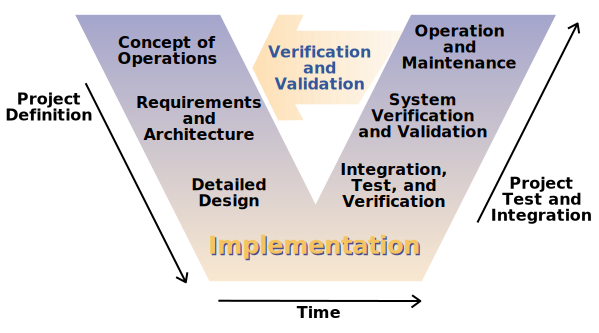
\includegraphics[height=70mm]{Figures/VandV}
  \end{center}
  \caption{Verification and Validation Diagram for a Systems
    Engineering Life Cycle \cite{vandv}}
\end{figure}
The left side of the V\&V diagram highlights all of the required
design while the right side details the build. 

\subsection{Interface Diagrams} 

Interface Diagrams (IDs) are important for many reasons. The biggest
reason that these diagrams are created and maintained is to create
visibility within each subsystem team in a systems engineering7
project. It is crucial that each member working on a project has a
general or even an expert understanding of each subsystem. During the
design process, it is important that each function of each subsystem’s
component is documented so that the current design selection is
recorded and so each of the member’s is familiar with each subsystem
and all of its functionalities. The following image is the ID for the
attitude control and maneuver electronics subsystem on the Gemini Spacecraft.  
\begin{figure}[H]
  \begin{center}
  \includegraphics[height=70mm]{Figures/ACME_ID}
  \end{center}
  \caption{ACME Interface Diagram from the Gemini Spacecraft\cite{qp10}}
\end{figure}
This is an example of an interface diagram for a small subsystem of a
large systems engineering project. The spacecraft requires several
subsystems to work together in the design and fabrication
process. Each of these subsystems has their own ID as well. This is a
good example to introduce you to what these diagrams are. The left
side of the image is the digital computer  which has an accumulator
which flows to the ladder logic block. From the ladder logic flows
several functions into both the attitude control and maneuver
electronics and attitude display blocks. This ID is simple since there
are only four components with many functions, however, many
complicated systems can have extremely complex diagrams. The Figure
below is an example of an ID for an entire spacecraft with all of the 
subsystems included in the diagram.
\begin{figure}[H]
  \begin{center}
  \includegraphics[height=70mm]{Figures/NewHorizons_ID}
  \end{center}
  \caption{New Horizons Interface Diagram\cite{qp11}}
\end{figure}
\subsection{Activity Diagrams}
Activity diagrams are similar to a flowchart.  It is a tool for
representing the sequence of Actions that describe the behavior of a
Block or other structural element. The sequence of execution is
defined using Control Flows. The Actions in an activity diagram can
contain Input and Output Pins which act as buffers for items that flow
from one action to another. Anything that can be produced, consumed,
or conveyed by the system is considered to be an item. Physical
materials, energy, power, data, and information are examples of items\cite{qp12}.

Activity diagrams are useful for engineering modeling.  It conveys
high-level functions and operations to the user. The main purpose of
an activity diagram is to draw the activity or action flow of a
system. Next, it is used to describe the sequence from one activity to
another. Finally, an activity diagram describes the parallel,
branched, and concurrent flow of the system \cite{qp13}.

Activity diagrams are important to the design process because they
maintain coherence throughout the project. If a system is composed of
multiple, intertwining subsystems, a person can simply follow the
activity diagrams to understand how each component and subsystem
interacts with one another. Activity diagrams also describe the data
flow of a system and when or where that data is created, converted or
used. Overall, activity diagrams are the roadmap of a system and
describe the intricacies of how it operates.  

As stated previously, activity diagrams denote how components and
subsystems interact with each other. This is accomplished through the
use of swimlanes which keep separate the individual activities and
object flows of a component or subsystem. Swimlanes are the boxes
which contain activities, however control and object flows can
traverse swimlanes. Activities which have inputs and outputs will also
have a pin attached to them. This small rectangular box denotes when
matter, energy or data flow is created or destroyed.  

The main purpose of activity diagrams is to show the control flow of
the system. This control flow refers to the execution path of an
activity. Control flow is indicated by control nodes for which there
are seven different kinds. Each control node is described in the table below.
\begin{table}[H]
  \begin{center}
    \begin{tabular}{c|p{7cm}|c}
      \hline
      Control Node & Description & Appearance \\
      \hline
      \hline
      Initial Node & The beginning of an activity sequence & Black
      circle \\
      \hline
      Activity Final Node & The end of an activity sequence & Black
      circle within a circle \\
      \hline
      Flow Final Node & The end of one branch of an activity sequence,
      but not the entire activity diagram. & Circle with an 'X' in it
      \\
      \hline
      Decision Node & The splitting point of an activity flow based on
      the outcome of a boolean operator such as ‘isCommandValid
      ==True’. One flow in comes in, while two flows come out as
      branching paths. & Diamond \\
      \hline
      Merge Node & The merging point of two activity paths. Two flows
      come in, while one flow comes out. & Diamond \\
      \hline
      Fork Node & The distribution of an activity flow into multiple
      pathways. When one object or control token comes in, it is
      duplicated into multiple paths. & Black bar \\
      \hline
      Join Node & The joining point of multiple synchronized
      concurrent flows. Two concurrent flows come in, while one flow
      comes out. & Black bar \\
      \hline
      \hline
    \end{tabular}
  \end{center}
\end{table}


\section{Guidance Navigation and Control Design for CubeSATs}

Every vehicle must be able to maintain a specific position within
its flight or orbit as well as point in a specific direction to achieve its mission. Mission goals have specific trajectories or orbits that must be reached and maintained, and this section is intended to explain how this is done from a guidance navigation and controls perspective. The basis for the guidance, navigation, and control (GNC) subsystem are attitude control, attitude estimation, and position estimation. Attitude describes which direction the vehicle is pointing in three-dimensional space. Attitude control is the act of controlling the orientation of the vehicle while attitude estimation is the process of determining the precise direction of the vehicle in order to perform attitude control. 

Vehicle State estimation is a fundamental portion of GNC and
requires the vehicle to determine it's orientation with respect to an
inertial frame as well as its position from an inertial reference
point. Some sensors are specific to the vehicle application but here
this section will discuss some of the major state estimation sensors.

Position estimation primarily involves integration schemes or GPS in order to determine the position of the vehicle on the surface of the planet. While performing the mission, the vehicle will continually use this subsystem to document the position. The basis of these techniques follows an understanding of spaceflight mechanics and systems engineering. Thus, the following approach will help garner a better understanding of an academic approach to the GNC subsystem and what methods are used to convey each component of the subsystem. 

The GNC subsystem is critical for the survival of the vehicle. It
is the system that determines the vehicles orientation and position
in space. Guidance is task of computing the desired trajectory and
orientation of a vehicle. Guidance is completed by using
components to determine any changes in position, altitude, or
orientation to assist the vehicle in following its projected
trajectory. Similar to guidance, navigation is the system's way of
leading the vehicle in space and keeping it on its intended
path. When people think of navigation they typically refer to Global
Positioning Systems (GPS) in their car or on their phones. This same
idea applies to aerospace systems as well. A GPS is a common device used for navigation on a vehicle and these components are discussed more further in this section. In order to have a successful flight and achieve the intended mission goal the vehicle needs to be stable and controlled in space. There are many different components different aerospace vehicles use to accomplish this. Satellites
use reaction wheels and gimbaled thrusters to name a few while
aircraft use aerodynamic surfaces.

\subsection{Trajectory Analysis}

The trajectory of a spacecraft is crucial to the GNC subsystem. The
type of orbit that the spacecraft is designed for plays a large role
in determining the components chosen for the attitude control,
attitude estimation, and position estimation.  

There are five main trajectories that spacecrafts typically follow:
\begin{enumerate}[itemsep=-5pt]
\item LEO  (Low Earth Orbit) - Things that must be taken into account
  in this trajectory are aerodynamics, Earth albedo, and space
  debris. 
\item MEO (Medium Earth Orbit) - Van Allen Belts, which are radiation
  belts, need to be considered during the design process. 
\item GEO (Geosynchronous Orbit) - Most communication satellites are
  in geostationary orbit since the satellite appears stationary and
  the communication dishes can be pointed directly at them and do not
  need to be maneuvered to follow the satellite. 
\item HEO (High Earth Orbit or Highly Elliptical Orbit) - In this case
  you might be well outside of the GPS constellation, thus, constant
  position must be considered by an alternate means. 
\item Deep Space - A deep space orbit is largely outside of any
  protective atmosphere, therefore radiation is a dominant
  concern. Also, well beyond the GPS constellation. 
\item Propulsion, magnetorquers, and reaction wheels are the three
  main mechanisms for controlling the attitude of the
  spacecraft. Reaction wheels can be used universally, however,
  magnetorquers are only useful within a magnetic field. Thus, within
  Low Earth Orbit (LEO) magnetorquers are incredibly useful, however
  in highly elliptical orbit (HEO) they may not be nearly as
  useful. As for the third option, propulsion, it is really only
  useful outside of a magnetic field when magnetorquers are not
  ideal. A middle Earth orbit (MEO) is unique in that it can use
  everything that is offered in the LEO and HEO but it will
  continually travel through the Van Allen Belts. The Van Allen Belts
  are pockets of radiation trapped by the Earth’s magnetic field which
  require additional shielding onboard the spacecraft to mitigate its
  effects.
\end{enumerate}

In LEO, it is common to use a Global Positioning System (GPS) to
estimate the position of the spacecraft. This component is most useful
at lower altitudes because it is able to reach the GPS signal,
however, as the altitude increases and the spacecraft moves farther
away from the signal, it is no longer helpful. This is when an
integration scheme may be the best possibility for position
estimation. Integration schemes, such as RK-11, are tedious but are
commonly used in HEO. Since HEO’s have an enormous apogee compared to
perigee, up to a 35:1 ratio, the need for an alternate means to
determine position is imperative\cite{cassidis}\cite{qp2}.  

Much like a HEO, any deep space trajectory will more than likely take
the spacecraft outside of the GPS constellation. Therefore, in order
to determine position the spacecraft must use NASA’s deep space
network, a numerical analysis, or another mathematical
means. Communication with the spacecraft is another complex variable
when in a deep space trajectory. Because of the large amount of
latency between the ground and the spacecraft, the spacecraft will
need to be able to autonomously operate without a constant uplink from
the ground. Lastly, the spacecraft will need additional radiation
shielding when in deep space to protect itself. This will further
increase its mass and add further constraints to the GNC subsystem. 

Attitude estimation can be determined by the use of magnetometers,
however, similar to magnetorquers, they are only useful within a
magnetic field. Thus, magnetometers are used when the spacecraft is
set to be in LEO. There are several methods that can be used for
attitude estimation, however, the only other one that greatly depends
on the orbit are horizon sensors which must be used in LEO.

\subsection{Spacecraft Environment}

The environment of space can have an enormous impact on the spacecraft
and the GNC subsystem. The environment is dependent on the trajectory
of the spacecraft and at what altitude it is set to reach. The
environment of space changes as the spacecraft travels farther from
the earth and there can be negative repercussions depending on the
components and materials chosen for the spacecraft.  

There are four main environments that may affect a spacecraft:
\begin{enumerate}[itemsep=-5pt]
\item Earth: Does not affect the design of the spacecraft but it is
  important to keep in mind that if components are not commercial off
  the shelf (COTS), they need to be built in a lab 
\item Launch: It is crucial to research the vibration requirements
  before launching. Again, if it is not commercial off the shelf, a
  vibe test must be run to ensure the components survive.  
\item LEO: This environment has many factors that must be considered
  including effects from the sun, thermal changes, Van Allen Belts
  which account for a large amount of radiation thus radiation
  shielding must be researched for the separate components. 
\item Deep Space: There are some things such as meteorites that may
  need to be considered, however, there is not much that can be
  done. This environment should not heavily affect the design.
Note that the spacecraft is going to undergo multiple types of
disturbances as explained in the dynamic model section.
\end{enumerate}

\subsection{Spacecraft Attitude Control}

Attitude control is the means by which the orientation of the
spacecraft is maintained within the orbit. Throughout the mission, the
spacecraft experiences disturbance torques that are caused by a
variety of sources, such as aerodynamics, gravity gradient, and solar
radiation pressure discussed previously. These torques impart momentum
which rotate the system away from its desired orientation. The purpose
of attitude control is to reject these disturbance torques while
simultaneously pointing towards a desired orientation. Possible active
mechanisms for attitude control are magnetorquers, reaction wheels,
thrust vector control, reaction control system, and control moment
gyros.

There are several components that can be used for the attitude control
of a satellite. Selecting the proper component is dependent on the
orbit and its apogee/perigee, the system's requirements, and the risks
associated with the component. There are several steps involved with
component selection. Typically the team will review the requirements
and perform a preliminary risk analysis. This will generally help
narrow down which components to use where. To determine the specific
component, trade studies are conducted to compare the components from
different manufacturers to determine the best one for the project at
hand.

\subsubsection{Magnetorquers}

The first option for attitude control is a magnetorquer. A
magnetorquer, or torque rod, is built from electromagnetic
coils. These coils produce a magnetic field that interacts with
another magnetic field, typically Earth’s, which in turn produces a
torque upon the satellite\cite{qp14}. These components are used for changing
the angular momentum of the satellite. In addition to attitude
control, magnetorquers are also used for detumbling the
satellite. Detumbling is a means of stabilizing the satellite after
being inserted into the desired orbit\cite{qp15}. The International
Geomagnetic Reference Field (IGRF) is a software that reports the
magnetic field of the earth by using latitude, longitude, and altitude
from a GPS. This magnetic field is then used to determine the proper
magnetic field required by the magnetorquer to maneuver the
satellite.

\begin{figure}[H]
  \begin{center}
  \includegraphics[height=40mm]{Figures/Magnetorquers}
  \end{center}
  \caption{Example Magnetorquer\cite{qp16}}
\end{figure}

An example of magnetorquer effectiveness is its ability to detumble
during an orbit, and how many orbits it will take to completely
detumble the spacecraft. First, the magnetorquer will have a magnetic
moment value associated with the physical parameters of the rod
$\mu$. First the average torque is computed by taking the magnetic
moment and multiplying it with the average field strength and the
point (from IGRF model). Then, this average torque is multiplied by
total time of the orbit $T_p$ to determine 
the magnetorquer’s momentum effectiveness over one orbit. Note that
the torque from the magnetorquer’s $\vec{M}_{MT}$ is substracted by
the total disturbance torques $\vec{M}_D$ to obtain the total
effectiveness of the magnetorquers. From this, it is possible to
calculate the number of orbits it will take to detumble the spacecraft
on an axis.  

\begin{equation}
  N_{orbits} = \frac{||\vec{H_S}||}{T_p(\vec{M}_{MT}-\vec{M}_D)}
\end{equation}

The magnetorquer effectiveness boils down to the difference in the
total moment that the magnetorquers can produce and the total
disturbance momentum during the orbit. Then, the number of orbits that
it will take for the spacecraft to detumble in an axis is a function
of the magnetorquer effectiveness divided by the initial angular
momentum in each axis.

\subsubsection{Reaction Wheels}

Reaction wheels are mechanical disks, or flywheels, that rotate the
satellite during orbit. The reaction wheels take in electrical power
and provide a torque to the satellite\cite{qp18}. This electrical power is
provided to a DC motor which then spins the reaction wheel. Because
momentum must be conserved, angular momentum must also be
conserved. Thus, by Newton’s third law, when the reaction wheel
rotates one direction the satellite rotates in the other. So, a
minimum of one reaction wheel is placed on each axis to control the
rotation in all directions. The primary role of a reaction wheel is to
point the satellite without the use of any fuel.
\begin{figure}[H]
  \begin{center}
  \includegraphics[height=40mm]{Figures/ReactionWheels}
  \end{center}
  \caption{Example Reaction Wheels\cite{qp19}}
\end{figure}

The inertia storage for reaction wheels is a parameter that can be
used to seek out the best reaction wheels for the spacecraft. Once the
inertia storage is computed, one can search for reaction wheels with
the proper amount of inertia storage required. For example, if a
reaction wheel with an inertia storage of 50 mNms is needed, one can
go to Blue Canyon Technologies website to find the datasheets for
their different reaction wheels. From there, it can be determined that
the best fit would be the RWP050 reaction wheels\cite{qp20}.

Once an estimate of the inertia of the satellite is obtained, they can
be used to compute the required inertia storage of the reaction wheels. The 
tip off rate for a spacecraft is the rate at which the spacecraft’s
angular velocity is altered due to its deployment. The following
equation shows how momentum can be calculated due to tip off.

\begin{equation}
||\vec{H}_S|| = max({\bf I}_S)\omega_{TOR}f
\end{equation}
where $\omega_{TOR}$ is typically set at 10 deg/s and f the factor of
safety is typically set to 2.

\subsubsection{Thrust Vector Control (TVC)}

When aerodynamic control surfaces are ineffective, TVC is a solution
to maintain the vehicle's correct attitude for the thrust duration. It
accomplishes this goal by gimballing (rotating) the thrust chamber or
by redirecting the exhaust-gas flow to develop torque \cite{qp21}. However,
thrust vectoring only moves the vehicle in two directions. TVC is
typically used to control pitch and yaw attitude on boosters and upper
stages.
\begin{figure}[H]
  \begin{center}
  \includegraphics[height=70mm]{Figures/TVS}
  \end{center}
  \caption{TVC Diagram\cite{qp22}}
\end{figure}

\subsubsection{Reaction Control System (RCS)}

Reaction control systems are small thrusters. These thrusters alter
the speed of the spacecraft's rotational or spinning motion. They are
good for making quick turns and are used for getting to new
orientations quickly. Reaction control thrusters are typically in
"couples" or pairs of thrusters that together can spin the spacecraft
without changing the lateral velocity. In addition, these thrusters
usually work great with reaction wheels. When reaction wheels slow
down, they produce a force. The RCS will oppose this force which
allows the spacecraft to remain in the intended
orientation\cite{qp23}.
\begin{figure}[H]
  \begin{center}
  \includegraphics[height=50mm]{Figures/RCS}
  \end{center}
  \caption{Example RCS Thruster \cite{qp24}}
\end{figure}

\subsubsection{Control Moment Gyro}

A CMG is a spinning rotor at a constant speed [25]. Similar to a
reaction wheel, a CMG also has a spinning fly-wheel controlled by a
brushless motor. However, the spin axis of a CMG can rotate with the
help of a second motor placed on a gimbal axis. If the angular
momentum can only rotate in a fixed plane, it is known as a single
gimbal control moment gyros (SGCMG). GMCS are usually more efficient
and produce higher torque than reaction wheels as the size of the unit
increases\cite{qp26}.
\begin{figure}[H]
  \begin{center}
  \includegraphics[height=50mm]{Figures/CMG}
  \end{center}
  \caption{Example CMG \cite{qp27}}
\end{figure}

\subsection{Spacecraft Attitude Determination}

Attitude determination is a fundamental portion of the ADACS board and
requires the vehicle to determine it's orientation with respect to an
inertial frame. The sections that follow detail the sensors and
fundamental attitude determination algorithms derived thus far. 

\subsubsection{Sensor Overview}

There are a multitude of sensors that are typically used on board
small sats. Note that most satellites use a combination of these
sensors rather than using all of them on one single satellite.

\begin{enumerate}[itemsep=-5pt]
  \item {\bf Magnetometers:} Only used in LEO, they measure the
    magnetic field in the body frame $\vec{\beta}_B = [\beta_x,\beta_y,\beta_z]^T$.
    \item {\bf Rate Gyros:} These sensors measure the angular velocity
      of the spacecraft in the body frame $p,q,r$.
    \item {\bf Solar Sensors:} These sensors can be coarse analog
      sensors with an accuracy of 45 degrees or can be high precision
      digital sensors that have accuracy down to 1 degree. Sun senors
      return an azimuth $\upsilon$ and declination $\delta$ angle which can be then
      translated into a vector in the body frame $\vec{S}_B$.
    \item {\bf Horizon Sensors:} Horizon sensors are typically used in
      LEO as they find the horizon of the Earth and use that for
      orientation information. These sensors also return an azimuth
      and declination angle that can be translated into a body frame
      vector $\vec{H}_B$.
      \item {\bf Startrackers:} Startrackers utilize a large aperture
        digital camera to photograph a starmap within the field of
        view of the lens. The photographed stars are then cross
        referenced with a starmap database and return the full
        quaternion vector.
\end{enumerate}

Some issues arise with all of these sensors. For example,
magnetometers must be activated when magnetorquers are turned off
otherwise those artificial magnetic fields will pollute the data. Rate
gyros are prone to drift while solar sensors can be quite
inaccurate. Startrackers also run the risk of being blinded by the Sun
and/or the Moon thus it is possible to design an
attitude determination algorithm that utilizes the Sun's ephemeris data
along with the Moon's ephemeris data in the event that the startracker
is obscured by the Sun/Moon.

\subsubsection{Inertial Measurement Unit}

An inertial measurement unit (IMU) is a combination of three
sensors. An accelerometer, rate gyro and magnetometer. A magnetometer
is a device that measures the local magnetic field in the body frame
$\hat{\beta}_{B} = [\hat{\beta}_x,\hat{\beta}_y,\hat{\beta}_z]^T$\cite{qp33}. Note that the $\hat{}$ implies a measurement rather than the truth signal. Measurements from sensors are prone to bias, drift, scale factor, misalignment, noise and other sources of error that must be accounted for.
\begin{figure}[H]
  \begin{center}
  \includegraphics[height=50mm]{Figures/Magnetometer}
  \end{center}
  \caption{Example Magnetometer \cite{qp34}}
\end{figure}
A rate gyroscope, commonly referred to as a rate gyro measures the
angular velocity also in the body frame $\hat{\omega}_{B/I}=[\hat{g}_x,\hat{g}_y,\hat{g}_z]^T$. 
\begin{figure}[H]
  \begin{center}
  \includegraphics[height=50mm]{Figures/RateGyro}
  \end{center}
  \caption{Example IMU with Integrated Rate Gyro \cite{qp35}}
\end{figure}
Accelerometers are sensors used to measure acceleration at a point P
on a rigid body $\hat{a}_{B/I}=[\hat{a}_x,\hat{a}_y,\hat{a}_z]^T$. For simplicity however, it
is assumed that point P on the rigid body is the center of mass point
C therefore the accelerometer is measuring the acceleration of the
body itself in the body frame with respect to an inertial frame
$B/I$. 
\begin{figure}[H]
  \begin{center}
  \includegraphics[height=50mm]{Figures/Accelerometer}
  \end{center}
  \caption{Example Accelerometer \cite{qp36}}
\end{figure}
As mentioned before, the IMU consists of 3 sensors all returning 3 measurments. This results in 9 scalar quantities being returned from this sensor which is where the term 9DOF gets it origin. In reality DOF means Degrees of Freedom which is contrary to the standard 6DOF simulation models explained above. However, the sensor community chooses to coin the term 9DOF to highlight the 9 different scalar values returned from IMUs. It is possible to obtain a 10DOF sensor which also returns pressure or temperature data. 

\subsubsection{StarTracker}

A star tracker is another critical component of attitude control. This
device is a camera that points out from one face of the satellite. The
camera is able to detect the stars in its field of view (FOV) and
determine the location of the satellite based on this. Specifically,
the star tracker images the “starscape” to identify the known planets
and stars, and compares the imaged locations to the known locations
using the SPICE Toolkit\cite{qp28}. NASA Jet Propulsion Laboratory (JPL) has
produced the SPICE Toolkit for knowledge of the location of the
planetary bodies and stars and specific times\cite{qp29}.
\begin{figure}[H]
  \begin{center}
  \includegraphics[height=50mm]{Figures/StarTracker}
  \end{center}
  \caption{Example StarTracker \cite{qp30}}
\end{figure}

\subsubsection{Sun Sensors}

A sun sensor is a device that senses the sun’s direction to measure
the position of the sun with respect to the sensor’s position. There
are three types of sun sensors. The first one is an analog sensor
whose output signal is a continuous function of the Sun angle. Next is
a sun presence sensor which provides a constant output signal when it
senses the sunlight. The last one is a digital sensor that produces
encoded discrete output that is measured by the sun angle function.

Sun sensors work based on the entry of light into a thin slit on top
of a rectangular chamber with the bottom part lined with a group of
light-sensitive cells. The chamber casts an image of a thin line on
the chamber bottom. The cells at the bottom of the rectangular chamber
measure the distance of the image and the refraction angle by using
the chamber height. The cells convert the incoming photons into
electrons and develop voltages which are converted into digital
signals. the direction of the sun can be computed when the sensors are
perpendicular to each other \cite{qp31}.
\begin{figure}[H]
  \begin{center}
  \includegraphics[height=50mm]{Figures/SunSensor}
  \end{center}
  \caption{Example Sun Sensor \cite{qp32}}
\end{figure}

\subsubsection{Horizon Sensor}

The horizon sensor is a sensor used by spacecraft in LEO to determine
the location of the Earth’s horizon. There are two main types of
horizon sensors: statics and scanning. A static horizon sensor is able
to detect the infrared radiation emitting from the Earth’s surface to
locate the horizon of Earth. Scanning horizon sensors are much more
complicated and use a system consisting of a spinning mirror to direct
light onto a bolometer. This bolometer can sense when the infrared
signal is present or lost. So, as the mirror rotates and reflects
infrared light into the bolometer, the bolometer is able to detect
when the signal is present or lost to determine the edge of the
horizon\cite{qp37}.  
\begin{figure}[H]
  \begin{center}
  \includegraphics[height=50mm]{Figures/HorizonSensor}
  \end{center}
  \caption{Example Horizon Sensor \cite{qp1}}
\end{figure}

\subsubsection{Deep Space}

As explained earlier, in deep space it is possible to obtain a vector
to the Moon to be used in the attitude determination algorithm. The
Moon sensor would give a vector to the Moon in the body frame
$\vec{M}_B$ while an inertial vector would be needed $\vec{M}_I$. This
inertial Moon vector could be obtained via the Moon's
ephemeris data which could be loaded onto the satellite's processor
and use the orbital elements of the Moon to determine its position
relative to the Earth. However, the Moon's ephemeris data would more
than likely give the Moon's position relative to the Earth
($\vec{r}_{\Earth \rightarrow \Moon}$). The vector $\vec{M}_I$ would
then be given by
\begin{equation}
  \vec{M}_I = \vec{r}_{\Earth \rightarrow \Moon} - \vec{r}_{B}
\end{equation}
where $\vec{r}_B$ is the satellite's position relative to the
Earth. Note however that the position of the satellite relative to the
Earth would need to be obtained via the Deep Space Network (DSN) and a
combination of state estimation by integrating the orbital
equations. The reference paper \cite{Munoz} is a great paper that
details all the different kinds of sensors and their algorithms. This
section will eventually be supplemented by the material in that
reference paper.

\subsection{Position Estimation}

Position estimation is for determining the placement or location of
the spacecraft in orbit. This can often be confused with attitude
estimation, however, this can be clarified with an analogy. A human's
posture is their attitude while their location, or place in reference
to something else, is their position. This analogy can be transferred
to spacecraft attitude and position. Position estimation is how
mission control determines the location of the spacecraft in space. It
is vital for the spacecraft to know its position in order for the on
board sensors to work as intended. Position estimation is similar to
attitude control in the sense that the orbit plays a large role in
determining the proper component. The major options for attitude
estimation are Global Positioning Systems and the Ground Station
Network. 

The Global Positioning System (GPS) was developed in order to allow
accurate determination of geographical locations by military and civil
users. It works by using satellites in Earth’s orbit to transmit data
which makes it possible to measure the distance between the satellites
and the operator. This form of signal communication is incredibly
accurate and used heavily for attitude estimation. Up to 30 GPS
satellites are currently in orbit, mostly in MEO, at altitudes around
20,000 km. There will be between four and eight of them above any site
on the Earth at any time\cite{qp38}. These satellites continuously emit
coded high-frequency radio signals which may be received by special
GPS receivers. These signals contain information about the exact
orbits of the satellites and the time of atomic clocks onboard. When
signals from three or more satellites are received, the GPS receiver
will compute the best possible location of the user by
triangulation. Much like when on Earth, a GPS can be used for
navigation in space. The GPS receiver on board the satellite will also
receive its longitude, latitude, and altitude as long as it is within
the GPS constellation.
\begin{figure}[H]
  \begin{center}
  \includegraphics[height=50mm]{Figures/GPS}
  \end{center}
  \caption{Example GPS Receiver \cite{qp32}}
\end{figure}

\subsection{Trade Studies}

Tradeoffs and considerations are analysis tools used to compare
different components. It is not always obvious which component is best
for a subsystem function. As shown in the previous sections, there are several
options for attitude control, attitude estimation, and position
estimation. It may not stand out at first glance which components are
the best, so it is up to the team to perform a proper tradeoff
analysis, a.k.a a trade study. What this typically looks like is a
comparison of the different parameters of the components. For example,
if the GNC team decides to look at an integrated system for attitude
estimation, a trade study can be conducted to compare the mass, power,
volume, and momentum storage for different Blue Canyon Technologies
XACT systems \cite{qp20}. It is important to keep this trade study organized
and regularly updated, so it is recommended that a table is created to
compare these parameters.  

The name “tradeoff” comes from the fact that for a system it is
typical that one feature must be compromised for the other. For
example, to get more power, it is probably reasonable to assume that
volume will be compromised because the size of the component will need
to increase to fit a larger power supply. Another example may be that
in order to increase the volume of a component to fit a larger
payload, the mass will be compromised and may increase. These
compromises especially become issues when they interfere with the
subsystem requirements.

\subsection{Risks}

Risk assessments are arguably the most important task for the GNC
team. It is crucial that the entire system is taken into consideration
and assessed for possible failures because only one part needs to fail
to cripple the whole mission. This includes non physical issues such
as increased lead times on parts for example. The purpose of a risk
assessment is to identify all possible risks, their severity and
likelihood and to come up with mitigation strategies for those risks. 

The purpose of risk assessments is to determine mitigation strategies
so that the identified risks may be prevented. These mitigations are
discussed amongst the team and heavily considered while designing the
subsystem. Mitigation strategies can range anywhere from simply
creating a preflight checklist to diverting control from one component
to another in the event of a failure. These strategies are the main
purpose of creating a risk analysis in the first place, so careful
deliberation should be used when creating them. 

The best way to conduct a risk assessment is by creating a risk table
for the GNC subsystem. A risk table will list out the possible risks
determined by the team and their subsequent mitigation strategies. It
will also list out the likelihood and severity of each individual risk
as decided by the team. These can be determined in any way deemed
reasonable by the team, but is most often used on a scale of one to
five for each category. These values can then be input into a risk
criticality matrix which shows which risks are of the greatest threat
level.  

It is important that risk statements are written in a specific way to
avoid any confusion or miscommunication between the different
subteams. A risk statement consists of four parts: the condition,
departure, asset and consequence. The condition is a single phrase
that describes the current key fact-based situation or environment
that is causing concern, doubt, anxiety, or uneasiness. The departure
describes a possible change from the design or plan. It is an
undesired event that is made credible or more likely as a result of
the condition. The asset is an element of the system or plan. It
represents the primary resource that is affected by the individual
risk. The consequence is a single phrase that describes the
foreseeable, credible negative impact(s) to meet performance
requirements. A proper risk statement should utilize these four parts
in a format similar to the following: “Given that [CONDITION], there
is a possibility of [DEPARTURE] adversely impacting [ASSET], which can
result in [CONSEQUENCE]”

\subsection{Conclusions}

The GNC subsystem's purpose is to know where the spacecraft is, where
it needs to go, and determine how it will get there. These
requirements are determined by the overall mission goal of the
spacecraft. The system constraints are divided into three main
categories: the attitude control, attitude estimation, and position
estimation. The attitude control is how the spacecraft will maintain
its current orientation during orbit. Magnetorquers, reaction wheels,
thrust vector control, reaction control systems, and control moment
gyros are all common components used to counteract the disturbance
torques and maintain the desired orientation. Attitude estimation is
how the spacecraft estimates its current orientation. This is commonly
achieved by star trackers, sun sensors, magnetometers, rate gyros,
accelerometers, and horizon sensors. Lastly, the position estimation
is knowing the precise location of the satellite during its orbit. GPS
and the GSN are the two most common methods for determining the
satellites position.  

Not only are the components important but one must also consider the
trade-offs and risks associated with the mission. Risks must be
assessed and properly mitigated in order to ensure the safety and
success of the spacecraft. This is done by creating risk tables using
if-then terminology.


\section{Radio Controlled Aircraft Design}

Many principles for large aircraft design can be applied to smaller
radio controlled aircraft but understand that many of the aerodynamic
principles are not quite well defined for slow and small
aircraft. These aircraft have low Reynolds number which often exhibits
odd phenomena. For example, airfoil selection is really not so much a
design point other than ease of manufacturing rather than maximizing
lift coefficient. Remember that Reynolds number can be defined from
the equation below where $\rho$ is the density at sea-level (1.225
kg/$m^3$ in SI units), $V$ is
the desired flight speed, $\bar{c}$ is the mean aerodynamic chord and
$\mu_{\infty}$ is the viscosity of air which in SI units is 1.81e-5
$kg/(m-s)$. 

\begin{equation}
Re = \frac{\rho V \bar{c}}{\mu_{\infty}}
\end{equation}

You can tell that flying a small aircraft ($\bar{c}$) and flying slow
$(V)$ results in a low Reynolds number. Either way the procedure below
has produced some great aircraft and the tools you'll learn along the
way will help you in your future aerospace engineering career. If
you're not an engineer then this text will at least give you an
appreciation for what goes into aircraft design. If you'd much rather
watch youtube videos than read this document, feel free to watch my
Youtube playlist on radio controlled aircraft design\cite{RCYoutube}

\subsection{Vehicle Type Selection and Requirements}

In the very beginning of your design you need to decide on the type of
aircraft you want to build. Designing a glider versus an aerobatic
airplane will result in vastly different engineering design
decisions. For example, a glider is going to have very long slender
wings while an aerobatic airplane is going to have somewhat shorter
wings with large control surfaces. I suggest you select from the
following types of aircraft and then move on: Gliders, Trainers, Sport
Aerobatic, Racers. If you'd like to build a scale aircraft there isn't
much to design since the shape of the aircraft is pretty much
built. If you do go with a scale aircraft this textbook isn't really
for you since you aren't really building a scratch build
aircraft. You're more just copying someone else's design. In that case
you may as well just buy a kit or watch some videos on balsa wood
construction and an overview of all the electronics required for RC
aircraft flight.

If you selected one of the other styles you're ready to move onto to
the next stage which is requirements. There is so much literature on
Systems Engineering, top level requirements, functional
requirements and derived requirements. The bottom line is you need to
determine what you want your aircraft to do. Do you want it to fly
straight up, upside down? Do you want the aircraft to be hand
launched? Land on a runway? Determine what you want the aircraft to do
and create a bulleted list of those requirements. Throughout the
design you can refer to these requirements and make sure you are
satisfying these requirements. If this is your first build then you
may just have one requirement and that is to take off and land without
crashing. But think a bit deeper. Do you want to turn the vehicle? Do
you want full channel control for roll, pitch and yaw or just yaw
control? Do you want landing gear? What sort of flying characteristics
do you want? Be as specific as possible here. 

\subsection{Initial Design - Hand Sketch and Aspect Ratio}

Once you have an idea of what the aircraft type is and what the
requirements are it's time to hand sketch your aircraft. Try and use
engineering paper, french curves, a ruler and a compass. Make this
hand sketch look nice so you can use it in your future design. Draw
your sketch to scale. You might be wondering, ``how do I draw the
aircraft without knowing what my wing loading or thrust to weight
ratio is?". The answer comes from my late aircraft design professor
Dr. Mikolowski (RIP). He would always say ``If it looks good, it flies
good". After designing so many aircraft and seeing so many scratch
builds from my students I can honestly say that this is true
100\%. If you're reading this now it means that there is already over
100 years of aircraft technology on the internet for you to research
and see what other aircraft look like. Make your aircraft look like
that but make sure it fits into your aircraft type and make sure it
satisfies your requirements from above. If one of your requirements
was to hand launch, then make sure your drawing reflects a vehicle
without landing gear and a place to grab the aircraft. If you wanted
full channel support make sure to include all the control
surfaces. Think about where you want the propulsion system to go and
how you're going to access the electronics before you fly. Think about
what you want the wing to look like. Make it as big as you think it
needs to fly. Use your intuition. This is an art. So much of
engineering is an art.

Once your aircraft sketch is complete (make sure to do a front view,
side view and top view of your aircraft), it's time to take down some
wing characteristics. This is why you need to draw your sketch to
scale. Measure the length of the wing (wingspan $b$) and the chord at the
root ($c_r$) and the tip ($c_t$). Compute the area of the wing ($S$) using
the area of a trapezoid or rectangle depending on the shape of your
wing. Once you have the wingspan and area you can compute the aspect
ratio of your aircraft.

\begin{equation}
AR = \frac{b^2}{S}
\end{equation}

The general rule is that the larger the aspect ratio the more
aerodynamically efficient your aircraft will be. This is why gliders
have very long and slender wings. At the same time, high aspect ratio
wings suffer from larger bending moments and can flex considerably in
flight. Finally, it's important to compute the mean aerodynamic chord
of the wing. This is basically the average chord of your wing. If you
create a rectangular wing your mean aerodynamic chord is just the
chord of the wing since it's constant. If not you'll need to integrate
over the length of the wing using the formula below where y = 0 is the
centerline of the vehicle and y=b/2 is the wingtip on the right
side\cite{caughey}. The parameter $c(y)$ is the chord length as a
function of y.

\begin{equation}
\bar{c} = \frac{2}{S}\int^{b/2}_0 c(y)^2 dy
\end{equation}

\subsection{Weight Estimate - Tabular Approach}

Once you have an idea of the overall shape it's time to estimate how
heavy the aircraft will be. First think about the fundamental
components of an aircraft. If you're not familiar with any of the
components below, just type the item into Google and you'll find
numerous articles and Youtube Videos about each component.

\begin{enumerate}[itemsep=-5pt]
\item ESC - Electronic Speed Controller
\item Battery - Assume for now that you'll be using a 1500mAh 3S 
  Battery unless you're building a micro aircraft in which case you
  might end up using a 600 mAh 2S or even a 300 mAh 1S. Think about
  the size of your aircraft. You will do more sophisticated battery
  design in the future.
\item Motor and Propeller - Again select something that is in the
  ballpark of the aircraft you're building. You'll do a redesign later.
\item Servos
\item Receiver
\item Control Linkages and Servo Horns
\item Fuselage
\item Main Wing
\item Tail both Horizontal and Vertical
\item Payload
\end{enumerate}

For each of the components above you need to estimate the weight of
these components. The only way to do that is to either look up the
weight of similar aircraft to the one you're designing or find
components that you think will work for your aircraft and add up all
of the weights. The most difficult part is going to be estimating the
empty weight of the aircraft which is just the structure of the
aircraft. For these estimates you need to decide what materials you
plan on using. Is your aircraft made out of foam, balsa, carbon fiber
or some type of combination. Perform an initial material selection and
then use that to estimate your weight. Create a table in a spreadsheet
type program or a numerical computer program so that you can go back
and change weights as your design progresses. Use the spreadsheet or
numerical program to compute the total weight of your aircraft. This
is your maximum takeoff weight.

\subsection{Airfoil Selection and 2D and 3D Lift}

The section \ref{s:aerodynamics} details the aerodynamic forces on the
aircraft. In this stage of design we will only be looking at the lift
equation.
\begin{equation}
L = \frac{1}2\rho {V}^2 S C_L
\end{equation}
The coefficient of lift $C_L$ is the lift coefficient of the
aircraft. This coefficient is a function of Reynolds number, angle of
attack, airfoil shape and wing shape. Recall that the angle of attack
is the angle between the zero lift line of the airfoil and the free
stream air. Breaking the velocity vector into components yields the
equation below where $w$ is the airspeed along the z-axis of the
vehicle and $u$ is the velocity along the x-axis. 
\begin{equation}\label{e:aoa}
\alpha = tan^{-1}\left(\frac{w} {u} \right)
\end{equation}
Using the angle of attack as a parameter, the lift coefficient can be
expanded to the following:
\begin{equation}
C_L = C_{L\alpha}(\alpha-\alpha_0)
\end{equation}
The parameter $\alpha_0$ is the angle of attack that results in zero
lift. This is a function of the airfoil shape. The parameter
$C_{L\alpha}$ is the lift curve slope and is a function of airfoil
shape, wing shape and Reynolds number. In order to remove, wing shape
from the design, the aspect ratio is used to convert the wing lift to
a sectional airfoil coefficient.
\begin{equation}\label{e:ar_equation}
C_{L\alpha} = \frac{C_{l\alpha}}{1+\frac{C_{l\alpha}}{\pi e AR}}
\end{equation}
The parameter $e$ is an efficiency parameter which is often assumed to
be 80-90\%. The coefficient, $C_{l\alpha}$ is the airfoil lift curve
slope which is different than the wing lift curve slope. The wing lift curve slope
will always be smaller than the airfoil lift curve slope. This is
because of an effect called wing tip vortices. Wing tip vortices are
an aerodynamic effect where high pressure from the bottom of the wing
moves around the wingtips to the area of low pressure. The only way to
mitigate these vortices is by installing winglets or increasing the
aspect ratio. Note that winglets increase drag and weight which is why
you don't typically see them on RC aircraft. The coefficient
$C_{l\alpha}$ is then simply a function of airfoil shape and
Reynolds number. This is what is often referred to as 2D lift. It is
the lift of airfoils which are two dimensional rather than 3D lift
which is over an entire wing. It is at this point that airfoil
selection and design can be used. The website \url{airfoiltools.com}
is a great resource for plotting lift curve slopes of various airfoil
shapes as a function of Reynolds number. I also have a great Youtube
video on how to use XFLR5 (pronounced X-Flyer
Five)\cite{XFLR5_tutorial}. A more comprehensive guide on XFLR5 can be
found in \cite{XFLR5_Guidelines} while the software itself can be
downloaded in \cite{XFLR5}. The basics of airfoil selection then break
down into the following 
process.

First, using your max takeoff weight and cruise flight speed, compute
the lift coefficient required in cruise. This assumes that lift equals
weight. 
\begin{equation}
C_L = \frac{2W}{\rho V^2 S}
\end{equation}
Then using your flight speed and chord length, compute the Reynolds number
of your aircraft. Use this Reynolds number and airfoiltools or XFLR5
to compute the sectional lift characteristics of various
airfoils. Airfoil selection can be as complicated as you make it but
you're looking for the highest lift to drag ratio airfoil. Another
simple way is to just select the airfoil with the highest sectional
lift coefficient. Another item to consider is manufacturing. Some
airfoils may be feasible for full sized aircraft but not for RC
flyers. My recommendation is to build an aircraft with a Clark-Y
airfoil. They are easy to cut with balsa or shape with foam and have
good lift to drag characteristics. Note that this airfoil is
cambered. If you want to fly upside down I suggest you use a symmetric
airfoil like a NACA 0012 or NACA 0014 is you need a bit more thickness
to fit a wing spar through the airfoil.
Once you have your airfoil selected, use the lift curve slope to
estimate $C_{l\alpha}$ by fitting a linear trend line to the portion
of the graph before stall. Also make sure to take note of what the
zero lift angle of attack is. You can then compute the wing lift curve
slope by using equation \ref{e:ar_equation}. Once you have
$C_{L\alpha}$, you can compute the angle of attack needed for
cruise. Make sure to convert $\alpha_0$ to radians before you use the
equation below.
\begin{equation}
\alpha = \frac{C_L}{C_{L\alpha}}+\alpha_0
\end{equation}
The resulting answer will be in radians and needs to be converted to
degrees to make sure you are not close to stall. Typically in cruise,
the angle of attack is only a few degrees with perhaps 8 degrees on
the high end. If the answer you receive is higher than that it can
mean a few things which may involve a redesign.
\begin{enumerate}[itemsep=-5pt]
  \item The simplest way to get more lift is to fly faster. The
    problem is you need a bigger motor which will increase your weight
    which will require more lift and more angle of attack. Flying
    faster will also change your Reynolds number. 
  \item You can increase the aspect ratio of your wing which will make
    your aircraft more efficient. The problem is that will increase
    the bending moment at the root creating the need for stronger
    materials at the root which also increases weight. This will also
    change your mean aerodynamic chord which will change your Reynolds
    number. 
  \item You can increase the area of the wing. This will also increase
    drag and weight but if the material you are using has a high lift
    to weight ratio then adding more wing area might be a good
    option. Depending on how you change the aircraft wing shape, the
    aspect ratio and/or the mean aerodynamic chord might change
    meaning you'll have to recompute the wing lift curve slope as well
    as the Reynolds number. 
  \item If you are using a symmetric airfoil it's possible you could
    forgo flying upside down and switch to a cambered airfoil which
    has more lift.
\end{enumerate}

Regardless of what you do make sure you angle of attack in cruise is
low which will reduce drag. It's optimal to fly at the aircraft's
highest lift to drag ratio but radio controlled aircraft don't
typically do that. It is also important to compute the stall speed of
your aircraft. You'd like this value to be as small as possible.
\begin{equation}
V_{stall} = \sqrt{\frac{2W}{\rho S C_{Lmax}}}
\end{equation}
In this case $C_{Lmax}$ is the maximum lift coefficient your aircraft
can obtain before stalling. If the stall speed is too high for your
design go back and redesign your vehicle. Once you have redesigned
your vehicle to fit within tolerable limits it's time to look at some
aircraft performance characteristics which include the W/S (wing
loading) and the T/W (thrust to weight ratio). 

\subsection{Wing Loading and Thrust to Weight Ratio}

The wing loading is defined as the weight of the aircraft over the
main wing area (W/S). Intuitively though, it is the amount of lift
required per square foot of wing area for your aircraft. If the wing
loading is high it means you have a heavy aircraft with small wings
which means you either need very high lift creating devices like flaps
and cambered airfoils or the aircraft needs to fly very fast. You can
imagine that warbirds and racers have higher wing loading then say a
glider which has very low wing loading. In this case the aircraft can
fly slow because the aircraft is light with larger wings. At this
stage of the design you already know the maximum weight of the
aircraft and the main wing area so it's simple to calculate. For
larger aircraft, there is a standard wing loading for aircraft as well
as another parameter called the wetted wing loading which is the
weight divided by the wetted area of the wing. The wetted area is
basically the surface area of the wing. For radio controlled aircraft
though the wing cube loading is used to ensure the aircraft is of the
correct type.
\begin{equation}
WCL = \frac{W}{S^{3/2}}
\end{equation}
Using the units of ounces for the weight and sqft for the area the
table below can be used to ensure that your aircraft is in the correct
ballpark\cite{WCL}.
\begin{table}[H]
  \begin{center}
  \begin{tabular}{cc}
    Type of Aircraft & WCL ($oz/ft^3$) \\
    \hline
    \hline
    Gliders & under 4\\
    \hline
    Trainers & 5-7\\
    \hline
    Sport Aerobatic & 8-10\\
    \hline
    Racers & 11-13 \\
    \hline
    Scale & over 15 \\
  \end{tabular}
  \end{center}
\end{table}
After computing your WCL it is possible that for the type of aircraft
you've designed, your value falls well outside the limits of the table
above. In that case you must redesign your vehicle by changing the shape
of the wings or choosing a different material to lighten up the
aircraft. In my experience, if you are designing a racer or scale
aircraft and you wing loading is smaller than above this is typically
ok so long as you have enough thrust to fly fast. In this case you may
just have a very fast trainer which isn't necessarily a bad thing. The
danger is when trying to design a glider with a WCL of over 15. That
aircraft will exhibit a very high stall speed and poor lift to drag
ratio (L/D) characteristics. Once you are satisfied with your WCL you
can move on to computing the thrust to weight ration (T/W).

For full-sized aircraft the T/W can range from 0.6 for passenger
aircraft all the way up to 1.2 or higher for get aircraft. For R/C
aircraft the same general rule applies. If your aircraft is a trainer
with landing gear you can probably get away with a T/W of 0.6 but I
would not recommend it. My recommendation would be to go no lower than
0.8 which would mean your maximum take off thrust is 80\% of your
maximum takeoff weight. In this configuration, the aircraft will
accelerate down the runway until just over stall speed at which point
the aircraft can takeoff. If you have strict runway requirements,
airborne requirements like vertical flight or loops and snap rolls, I
recommend increasing the size of your motor, ESC, battery, propeller
combination to yield a T/W of at least 1.2. In this case, even if your
wings are not very efficient, you can fly on thrust alone. You may not
exhibit great aerodynamic performance and still have a high stall
speed but worst case you can land the aircraft like a harrier which
I've done before.

Once you've selected your T/W you need to go find a
battery/ESC/motor/propeller combination that yields the thrust you
need. Tiger Motors website is typically very good at listing the
motor, propeller and battery combination to give you a certain amount
of thrust. Unfortunately, the hobbyist market is not using standard
engineering units and thrust is reported in grams. My recommendation
then is to use the following formula to compute your thrust required
in grams. This assumes that 4.44 N = 1 lbf and that you are on Earth
with 9.81~$m/s^2$ of gravitational acceleration. It'd be nice if the
community just reported thrust in lbf but alas that is not the case. 

\begin{equation}
T_{grams} = (T/W)W_{lbf}/453.59
\end{equation}

Remember, when selecting a propulsion system, you will need to go back
and update your weight estimate with the new values you've
obtained. This may effect your wing area slightly and may even require
you to choose a new motor if you were very off the first time you
estimated the weight. This is an iterative process and every step
builds on the previous step. The hope is that each iteration is not
very different than the last.

\subsection{Battery Sizing}

For battery sizing, you need to make sure the battery voltage is not
too high for the ESC or the motor. Typically the ESC and motor will
have a voltage limit listed on there. For example, an ESC that can
handle 3-6S LiPos can handle anywhere from 12.6V to 25.2V. Motors may
have different constraints than the ESC. It's also important to make
sure that you look up the maximum current in the motor and that number
must be less than the maximum current rating of the ESC. To compute
flight time at max throttle use the equation below

\begin{equation}
  \frac{mAh/1000}{A_{max,motor}} = TOF_{hours}
\end{equation}

where $mAh$ is the number of milliamp hours of your battery,
$A_{max,motor}$ is the max current draw of your motor at full throttle
and $TOF_{hours}$ is the time of flight in hours. Note that you can
repeat the calculation for different throttle settings provided you
know the current through the motor. 

You also need to make sure that the battery can output the necessary
current your motor needs at full throttle. The equation below is used
to ensure the battery can supply the necessary current. 

\begin{equation}
\frac{mAh}{1000}C > A_{max,motor}
\end{equation}

In the equation above, $C$ is the C rating of the battery usually
listed on the battery itself or in the product description.

\subsection{Stability and Control, Center of Mass, Aerodynamic Center and Static Margin}

Stability and Control is a very large section of literature and could
be taught over an entire semester. Stability just ensure the aircraft
flies steady and level and is typically broken up into lateral (side
to side) and longitdutinal (front to back) stability. Lateral
stability in my opinion is more complex but to ensure you aircraft is
laterally stable, just be sure your aircraft is symmetric about the
left and right planes and also be sure that your tail surface provides
adequate yaw stability through the use of a vertical tail or a V-tail
if you opted for a combined control surface. Longitudinal stability
involved two more calculations that must be done before the aircraft
can be built. These two parameters are the center of mass and the
aerodynamic center. The center of mass is a very simple quantity to
compute by just using the center of mass formula shown below.
\begin{equation}
x_{cm} = \sum\frac{x_iW_i}{W}
\end{equation}
In the equation above, $x_i$ is the distance of a component from a
reference point on the aircraft. I typically use the nose of the
fuselage as the reference point. For standard aircraft the motor would
have a negative distance from the reference point and the receiver and
battery would have a positive value. The value $W_i$ is then the
weight of each component. Placing servos, receivers and other
electronics is a design parameter to move your center of mass while
the fuselage is typically a parameter that must be estimated at this
stage. My recommendation is to break the aircraft into fuselage, tail
boom, tail and main wing components and treat each one as a
component. You will notice that moving the main wing and battery
drastically changes the center of mass.

The next parameter is the aerodynamic center. The main wing looking
from the top is basically a 2D distributed load. As such the center of
lift must be computed. Assuming the main wing is symmetric, the
aerodynamic center will lie on the center line of the aircraft. In
this case the problem reduces to a 1D computation. In order to compute
the center of lift along the x-axis (pointing towards the nose) you
need to compute the weighted average of the center of lift of each
airfoil. In this case if you have a symmetric airfoil, the center of
lift is 1/4 of the chord length. If you have a cambered airfoil the
center of lift is typically in the 30\% range so you can use 25\% for
a symmetric airfoil and something slightly larger for a cambered
airfoil. Once you determined the center of lift for the airfoil you
can use the equation below for the aerodynamic center of the entire
wing\cite{AndersonD,caughey}.
\begin{equation}
x_{ac} = \frac{2}{S}\int^{b/2}_0 x_{af}(y)c(y) dy
\end{equation}
The parameter $x_{af}(y)$ is the location of the center of lift of the
airfoil as a function of y. Once you have the aerodynamic center and the
center of mass you can compute the static margin of your aircraft.
\begin{equation}
S_{m} = \frac{x_{ac}-x_{cm}}{\bar{c}}
\end{equation}
The value of the static margin is not as important as the sign. If
measuring from the nose of the aircraft the aerodynamic center must be
behind the center of mass. To explain this think about stable
aerodynamic vehicles like darts, or arrows. Notice that darts and
arrows have fletching in the rear to create aerodynamic surfaces
farther back. Unstable vehicles like frisbees and footballs have
aerodynamic centers in front of the center of mass in which case they
must spin in order to provide stability just like a bike tire or a
dreidel. Using the equation above, if $x_{ac}$ is behind $x_{cm}$ it
means that $x_{ac}$ is bigger or more positive than $x_{cm}$ in which
case your static margin would be positive.
\begin{equation}
\begin{Bmatrix} S_m>0,~stable \\ S_m<0,~unstable \end{Bmatrix}
\end{equation}
If you perform these two calculations and find your static margin to
be negative it means that you need to shift your battery and other
components more towards the nose or move your wings backwards. Note
that moving your wing backward will also shift your center of mass so
try and move some components forward before shifting your wings
around.

The final stage of this design is Control. Aircraft in flight require
3 control surfaces to provide roll, pitch and yaw control. These
include the aileron, elevator and rudder. It's possible to fly
aircraft without a rudder by performing a ``bank and yank" maneuever
and it's also possible to combine elevators and ailerons into
something called elevons. I've even seen some ruddervators. Whatever
you decide to do make sure that you can adequately control all three
axes or if one axis is uncontrollable be sure that that axis is
stable. I've seen some aircraft that only have rudder and elevator and
no ailerons. I find these aircraft hard to control but the idea is you
move the rudder to yaw the aircraft which also rolls the aircraft
allowing you to turn. It creates a very slow aircraft but it also
reduces complexity if that is something you're interested in doing.

\subsection{Iteration, Detailed Sketch and Final Checks}

This section in my opinion is absolutely essential. It involves going
back and making sure that your current design satisfies your
requirements you originally wrote in the first section of this
design. Recompute your aspect ratio, and update your weight estimate
based on any calculations you've obtained. This may be finding better
estimates for parts or materials. You also need to create a better
sketch and determine where EVERY component is going to go and what
sort of support you will need. If you're building your aircraft out of
balsa you will need detailed sketches on rib, spar and stringer
placement. All of these updates will change your weight estimate which
will change your WCL and your T/W. Be sure your WCL and T/W are within
tolerable bounds. You also need to go back and compute you angle of
attack during cruise and be sure you are not in a stall regime. Be
realistic with your flight speed as well during cruise. Go back and
compute your stall speed. Is it realistic? If not then go back and
make some minor changes. Finally, be sure you aircraft is
longitudinally and laterally stable and that you can control all 3
axes or at least the uncontrollable axes are stable. Once you are
certain the aircraft will fly you can begin purchasing components. 

\subsection{Computer Aided Design (CAD)}

This section is optional but sometimes it's just nice to have a CAD
view of your aircraft especially if you are 3D printing parts or
perhaps getting some component machined out of aluminum. Some CAD
programs are even so powerful they will compute bending loads, center
of mass and even drag. Use whatever tools are at your disposal to help
you in the design. 

\subsection{Purchase Components}

I wanted to write an entire section on purchasing component to go over
a few common mishaps. First, if you are using a LiPo battery be sure
to familiarize yourself with the dangers of LiPo batteries. I've
almost caught my entire lab on fire by charging a damaged LiPo but all
batteries can technically catch fire. Please be careful. Furthermore,
be sure you purchase an ESC with the right current rating. If you
overload an ESC with too much current it will also catch on fire. The
servos you buy have a torque rating. Be sure your servos can overcome
the aerodynamic torque estimated in flight. Generally servos are sized
by the size of the aircraft so you can just purchase servos that are
designed for your particular size aircraft. The motor you purchase is
going to need a mounting point. Consider designing a motor plate or
even a firewall depending on the type of aircraft. When purchasing
materials make sure to get them from a good brand. Companies like
Flite Test sell really good double plated foam that is designed for RC
aircraft. Purchasing Dollar Tree foam board is totally acceptable but
just understand that after a crash or two the foam board won't work
anymore. Also consider what type of glue you are planning on
using. Certain types of glue can actually melt foam and hot glue can
melt certain types of foam as well. CA glue is very good for balsa but
will melt foam. Two part epoxy is strong but it weighs more than CA
glue and takes a long time to set compared to other types of
glue. Also be sure to be lenient on glue where you can. Glue just adds
weight and that will reduce your performance. Finally, make sure your
receiver supports the number of servos you plan on using and be sure
that your transmitter and receiver are compatible. All of my aircraft
use Spektrum technology but you may opt to use a different type of
protocol.

Finally, when all components come in be sure to test them. DOA stands
for dead on arrival and so many components come DOA. Before you spend
the time to install all your components in your aircraft and then
throw the aircraft in the air make sure you test every component and
be sure it works. I also suggest weighing each component on a small
scale and updating your weight estimate to ensure everything is within
tolerable bounds. 

\subsection{Building}

Once you have all necessary resources to build your aircraft I
recommend starting with the fuselage or main wing and then installing
all componets. I recommend taking pictures of your build in case you
need to reference them later. Go slow. If you break something it will
be expensive. Also remember that if the aircraft looks good it flies
good. This means that gluing all components properly and having the
aircraft be as smooth as possible will translate to better flight
performance. 

\subsection{Flying}

Before you fly I recommend finding a pilot will more experience than
yourself to check out the aircraft and make sure the aircraft has been
built properly. You may even want to discuss your initial design
before you even begin building to make sure there are no major
critical issues. If you want to fly the aircraft yourself I suggest
flying an aircraft using a simulator. My recommendation is the free
program CRRCSim\cite{CRRCSim}. It is not a great simulator by any means but it will
at least familiarize yourself with aircraft controls. Before you fly
make sure to build yourself a pre and post flight check list. I've
included my pre and post flight check list that I use before every
flight test.

\subsubsection{Day Before Flight Checklist}
\begin{enumerate}[itemsep=-5pt]
\item Assess the weather to ensure acceptable flight conditions
  \begin{enumerate}[itemsep=-5pt]
    \item No strong winds (anything over half your stall speed is too fast)
    \item No rain or lighting
  \end{enumerate}
\item State and confirm the purpose of the flight test - Set clear
  goals the aircraft should complete before test 
\item Check for damage to the plane and if the moving parts are secured including motor and electronic speed control and all components
\item Check for a full battery charge on plane and controller; charge
  all electronics if not fully charged
\item Perform Ground Safety Check List
\item Take note of items that need to be repaired even if the flight test is not implemented
\end{enumerate}

\subsubsection{Ground Safety Check List}
\begin{enumerate}[itemsep=-5pt]
  \item Ensure that propellor is off
  \item Turn on TX
  \item Connect battery to aircraft
  \item Ensure all control surfaces are operational and moving the
    correct way
  \item Spin up motor and be sure that motor is spinning the correct
    way
  \item Perform a range check where pilot moves control surfaces with
    50\% or more throttle while walking away from aircraft. Ensure that pilot can move at least
    300 feet away without any dropouts.
  \item Remove battery and install propeller
  \item Reconnect battery.
  \item Using safety glasses, apply full throttle to TX and ensure
    that adequate thrust is generated to fly aircraft. Leave full
    throttle applied for at least 30 seconds to be sure no component. 
    fails. Better to fail on the ground than in the air.
\end{enumerate}

\subsubsection{Preflight Checklist}

\begin{enumerate}[itemsep=-5pt]
\item Perform all “Day Before Flight” Checks
\item Perform Ground Safety Checks
\item Check for any damage to any components including the battery
\item Install Prop
\item Turn on TX
\item Plug in main battery
\item Confirm flight time and range distance
\item Clear obstructions and make sure there is clear space for takeoff and landing
\item Arm TX if the TX has an arm switch
\item Ensure all control surfaces are operational and moving the correct way
\item Apply throttle and fly
\item Upon landing do everything in reverse order
\end{enumerate}

\subsubsection{Post Flight checklist}
\begin{enumerate}[itemsep=-5pt]
  \item Check plane for any damage
  \item Check all moving parts are still secured
  \item Check for battery overheating, discoloration, warping, or swelling
  \item Check battery usage with a voltmeter
  \item Check if the plane is able to power on again
  \item Have PIC (pilot in command) give a post flight assessment
  \item Put batteries in LiPo storage
\end{enumerate}

\section{Helpful Aircraft Equations}

\begin{multicols}{2}

\noindent Mach Number and Reynolds Number

\beq
\beqn
M_{\infty} = \frac{V}{a_{\infty}} \\
\ \\
Re = \frac{\rho V \bar{c}}{\mu_{\infty}}
\eeqn
\eeq

\noindent Total Velocity

\beq
V = \sqrt{u^2 + v^2 + w^2}
\eeq

\noindent Angle of Attack and Sideslip

\beq
\beqn
\alpha = tan^{-1}\left(\frac{w}{u}\right)\\
\beta = sin^{-1}\left(\frac{v}{V}\right)
\eeqn
\eeq

\noindent Lift Drag and Moment

\beq
\beqn
Lift~(L) = \frac{1}{2} \rho V^2 S C_L \\
Drag~(D) = \frac{1}{2} \rho V^2 S C_D\\
Roll~Moment~(L) = \frac{1}{2} \rho V^2 S b C_l\\
Pitch~Moment~(M) = \frac{1}{2} \rho V^2 S \bar{c}C_m\\
Yaw~Moment~(N) = \frac{1}{2} \rho V^2 S b C_n\\
\eeqn
\eeq

\noindent Lift and Drag Coefficients

\beq
\beqn
C_L = C_{L0} + C_{L\alpha}\alpha\\
C_L = C_{L\alpha}(\alpha-\alpha_0)\\
C_D = C_{D0} + C_{D\alpha}\alpha^2 \\
C_D = C_{D0} + k{C_L}^2 \\
\eeqn
\eeq

\noindent Non-dimensional Angular velocities

\beq
\beqn
\hat{p} = pb/2V\\
\hat{q} = q\bar{c}/2V\\
\hat{r} = rb/2V
\eeqn
\eeq

\noindent Pitch Moment equation

\beq
C_m = C_{m0} + C_{m\alpha}\alpha + C_{m\delta_e}\delta_e +
C_{mq}\hat{q}
\eeq

\beq
\beqn
C_{m0} = C_{MAC} + C_{L0}\bar{x}_{sm} \\
\bar{x}_{sm} = \frac{x_{cg}}{\bar{c}} - \frac{x_{acW}}{\bar{c}} \\
C_{m\alpha} = \left(C_{L\alpha,W} +
\frac{S_t}{S}C_{L\alpha,t}\right)\bar{x}_{sm} - V_HC_{L\alpha,t}\\
V_H = \frac{l_tS_t}{S\bar{c}} \\
C_{m\delta_e} = \left(C_{Lt\delta_e}\frac{S_t}{S}\right)\bar{x}_{sm}-V_HC_{Lt\delta_e}\\
C_{mq} = 2C_{L\alpha t}\frac{l^2}{\bar{c}^2}
\eeqn
\eeq

\noindent Max Lift to Drag Ratio (Only valid if ${C_{L0}=0}$)

\beq
\alpha_{max,L/D} = \sqrt{\frac{C_{D0}}{C_{D\alpha}}}
\eeq

\noindent Lift to Drag when $T=0$ (Sum of Forces still zero)

\beq
\beqn
\frac{D}{L} = tan(\alpha)\\ %%%Where does this come from? Sum of Forces = 0
Lcos(\alpha) + Dsin(\alpha) = W
\eeqn
\eeq

\noindent Airfoil and Wing Aerodynamics

\beq
\beqn
x_{ac} = c/4 & 
a = \frac{a_0}{1+\frac{a_0}{\pi e AR}} \\
AR = \frac{b^2}{S}
\eeqn
\eeq


\noindent Standard Atmosphere

\beq
\beqn
\rho = 1.225~kg/m^3 = 0.00238~slugs/ft^3\\
\mu_{\infty} = 1.81x10^{-5}~kg/(m-s)\\
a_{\infty} = 331.3~m/s
\eeqn
\eeq

\noindent General Notes

\begin{enumerate}
  \item In trim or steady and level or cruise $q=0$, $C_m=0$,$L=W$, $T=D$
  \item For symmetric airfoil $C_{MAC} = 0$ and
    $C_{L0}=0$ thus $C_{m0} = 0$
  \item For a flat plate all symmetric properties apply but
    $a_0 = 2\pi$
  \item Tail surfaces are always assumed to be flat plates
  \item For longitudinal problems, $\beta = 0$ so $v=0$ (side velocity)
\end{enumerate}

\end{multicols}


%%%%%%%%%%%%%%%%%%%%%%%%%%%%%%%%%%%%%%%%%%%%%%%%%%%%%%%%%%%%%%%%%%%

\bibliographystyle{unsrt}
\bibliography{../papers.bib}

\end{document}
